% !TEX encoding = IsoLatin

% To print by both sides
%\documentclass[b5paper,11pt,twoside,cucitura]{toptesi}

% To print by one side
\documentclass[a4paper,12pt,cucitura]{toptesi} % Page and font size

\usepackage[a4paper,top=4.3cm,bottom=5.5cm,left=3cm,right=3cm,bindingoffset=5mm]{geometry}

\usepackage{lipsum}
\usepackage{amsmath}
\usepackage[linesnumbered,ruled]{algorithm2e}
%\usepackage{subfig}
\renewcommand{\figurename}{Fig.}
\usepackage{listings}
\usepackage{color}

% ADDED NOW
\usepackage{float}
\usepackage{ulem}
\usepackage{hhline}
\usepackage{amsmath}
\usepackage{ragged2e}
\usepackage{bookmark}
\usepackage{comment}
%\usepackage{subfigure}
  
\definecolor{codegreen}{rgb}{0,0.6,0}
\definecolor{codegray}{rgb}{0.5,0.5,0.5}
\definecolor{codepurple}{rgb}{0.58,0,0.82}
\definecolor{backcolour}{rgb}{1,1,1}
  
\lstdefinestyle{mystyle}{
    backgroundcolor=\color{backcolour},   
    commentstyle=\color{codegreen},
    keywordstyle=\color{magenta},
    numberstyle=\tiny\color{codegray},
    stringstyle=\color{codepurple},
    basicstyle=\footnotesize,
    breakatwhitespace=false,         
    breaklines=true,                 
    captionpos=b,                    
    keepspaces=true,                 
    numbers=left,                    
    numbersep=5pt,                  
    showspaces=false,                
    showstringspaces=true,
    showtabs=false,                  
    tabsize=2}
  
\lstset{style=mystyle,
    frame=single}

\usepackage{hyperref}

\hypersetup{
    pdfpagemode={UseOutlines},
    bookmarksopen,
    pdfstartview={FitH},
    %colorlinks,
    %linkcolor={blue},
    %linkcolor={black},     % Secretary version
    %citecolor={red},
    %citecolor={black},     % Secretary version
    %urlcolor={black}       % Secretary version
    %urlcolor={blue}
  }

\usepackage[latin1]{inputenc}% per macchine Linux/Mac/UNIX/Windows; meglio utf8
\usepackage[T1]{fontenc}\usepackage{lmodern}
\usepackage[intoc,english]{nomencl}
%%%%%%%%%%%%%%%%%%%%%%%% Glossary
\usepackage[toc]{glossaries}
\renewcommand*{\glstextformat}[1]{#1}
%\renewcommand*{\glstextformat}[1]{\textcolor{black}{\textbf{#1}}}          % Secretary version  
\makeglossaries


\begin{document}


%%%%%%%%%%%%%%%%%%%%%%%% List of Abbreviations
\makenomenclature
%\renewcommand{\nomname}{List of Abbreviations}

\english

\ateneo{Politecnico di Torino}
%\nomeateneo{Sede Centrale}
%\FacoltaDi{Department of Automation and Informatic??}
\titolo{A Social Bot for Personalized Recommendations of Bike Availability}
\sottotitolo{A study on Natural Language Understanding and Personalization}
\corsodilaurea{Computer Engineering}
\candidato{Martino \textsc{Mensio}}
\relatore{Prof.\ Maurizio Morisio}% per la laurea e/o il dottorato
%\secondorelatore{Prof.\ Claudio Casetti}% per la laurea magistrale
%\terzorelatore{{\tabular{@{}l}dott.\ Neil Armstrong\\prof. Maria Rossi\endtabular}}
\tutoreaziendale{Ph.D.\ eng.\ Giuseppe Rizzo}
%\NomeTutoreAziendale{Supervisore aziendale\\Centro Ricerche FIAT}
%\sedutadilaurea{Agosto 1615}% per la laurea quinquennale; oppure:
%\sedutadilaurea{\textsc{Anno~accademico} 2016-2017}% per la laurea magistrale
\sedutadilaurea{\textsc{Academic~year} 2017-2018}
\sedutadilaurea{\textsc{April} 2018}
\logosede{logopolito} % auxiliary ShareLaTeX logo

% Comment the following lines if you don't care about the title page in English
% Change the strings if you want a title page and a copyright page in another language
% Comment just the \iflanguage statement and the closing line of the language test
%	 if you want to make a global change instead of a conditional one.
%%%%%%%%%%%%%%%%%%%%%%%%%%%%%%%%%%%%%%%%%
  \iflanguage{english}{%
  %\retrofrontespizio{This work is subject to the Creative Commons Licence}
  %\DottoratoIn{PhD Course in\space}
  %\CorsoDiLaureaIn{Master Degree Course in\space}
  % TODO Master's Degree oppure Master of Science
  \CorsoDiLaureaIn{Master of Science in\space}
  %\NomeMonografia{Bachelor Degree Thesis}
  \TesiDiLaurea{Master's Thesis}
  %\TesiDiLaurea{Tesi di Laurea Magistrale}
  %\NomeDissertazione{PhD Dissertation}
  \InName{in}
  \CandidateName{Candidate}% or Candidate
  \AdvisorName{Supervisor}% or Supervisor
  \TutorName{Tutor}
  \NomeTutoreAziendale{Internship Tutor}
  %\CycleName{cycle}
  \NomePrimoTomo{First volume}
  \NomeSecondoTomo{Second Volume}
  \NomeTerzoTomo{Third Volume}
  \NomeQuartoTomo{Fourth Volume}
  }{}



%%%%%%%%%%%%%%%%%%%%%%%%%%%%%%%%%%%%%%%%%
%%%%%%%%%%%%%%%%%%% Front page
\frontespizio


%%%%%%%%%%%%%%%%%%%%%%%%%%%%%%%%%%%%%%%%%%%%%%%%%%%%%%%%%%%%%%%
% turns off chapter numbering and uses roman numerals for page numbers
\frontmatter
\pagenumbering{roman}

% CITAZIONE - PERSONALIZZARE
% VSPACE - PROPORZIONE USATA PER CENTRATURA VERTICALE DEL TESTO
% FLUSHRIGHT - ALLINEAMENTO ORIZZONTALE A DESTRA
%\vspace*{\stretch{1}}
%\begin{flushright}
%\noindent
%%\textit{To my family, I will be forever in his debt.}
%\textit{To my family, I will be forever in their debt.}
%
%%\textit{Docker Book}
%\end{flushright}
%\vspace*{\stretch{6}}
%
%\cleardoublepage
%%
%\vspace*{\stretch{1}}
%\begin{flushright}
%\noindent
%\textit{"To those who try, whether they fail or succeed."}
%
%\textit{Adrian Mouat}
%\end{flushright}
%\vspace*{\stretch{6}}

%%%%%%%%%%%%%%%%%%%%%%%%%%%%%%%%%%%%%%%%%%%%%%%%%%%%%%%%%%%%%%%
% ABSTRACT - PERSONALIZZARE
\sommario
%% !TEX encoding = utf8
% !TEX root = ../main.tex

% This content has been generated automatically from https://www.docx2latex.com/docx2latex_free and https://github.com/MartinoMensio/doc2latex_process_chapters 
% Consider editing the source Google Doc instead of this one!



\section*{Context}
Conversational agents are now, more than ever, the answer to establish a seamless interaction between end users and any service out there. The spreading of these agents, also called \textit{bots} or \textit{chatbots}, has highlighted an important need: going beyond the simple (often pre-computed) answer and provide personalized answers according to users' profiles.

This work contains therefore two major themes - Natural Language Understanding (NLU) and personalization - that follow each other's in a traversal argumentation from the literature to the selected approaches.

The \textit{Natural Language Interface} enables a communication with the machine in the language that is really used by humans in their everyday interactions with other people. Traditional mobile applications force the human to imitate the computer to exchange information, performing precise questions in the form of commands. The goal of Conversational Interfaces instead, is to reverse this imitation process in order to bring the interaction closer to the users using his natural language.

Once this interaction channel is ready, with the mutual understanding of the involved parties, a process of \textit{personalization} can be applied in order to provide user-centric contents and interactions.

\section*{Goals}
The goals of this work are of two different natures: \textit{i)} analyze the State of the Art in order to identify the approaches that better suit the creation of a Conversational Agent \textit{ii)} build a bot prototype that uses the selected approaches.

The first goal includes the two main themes: Natural Language Understanding and personalization. For the first one, the focus stands on Recurrent Neural Network (RNN) approaches that can perform a sentence classification (intent detection task) and extraction of parameters (slot filling task). The literature also shows how the input words can be used, by exploiting features (word embeddings~\cite{pennington2014glove}) computed on large datasets of unlabeled text, to capture syntactic and semantic similarities on big dictionaries. These similarities allow to be more robust towards words that have not been considered in training sets. For the personalization theme instead, the Content-based and Collaborative filtering are explained along with available methods to extract user features. These user features can be of anagraphic type or can be more undeclared traits such as Big Five Personality Traits~\cite{goldberg1993structure} that can be computed by analyzing external data coming from social networks and interests.

The second goal, the running prototype, is focused on the only theme of Natural Language Understanding. As use case the domain of urban mobility is chosen, having as specific objective the design and implementation of a Conversational Agent to retrieve real-time information about the bike sharing system. The bot should offer capabilities to find bikes given the user location, or plan trips between different points of a given city, using the data from the bike sharing providers. To provide a natural interaction with a user, the bot should be able to process requests that are not in the strict form of commands, but in a more conversational fashion. To reduce the distance between the system and the user, the bot should support multilinguality, to increase the usability of the tool for audiences belonging to different nationalities; for this reason both English and Italian languages are targeted with the prototype.

\section*{Personal contributions and results achieved}
Moving on the fulfillment of these goals, the approach is structured as follows. Firstly the description focuses on Natural Language Understanding, describing the selected approach to target two types of interactions (single-turn where each sentence is processed independently and multi-turn where an interaction context exists): for the single-turn interactions the reference State of The Art joint approach~\cite{liu2016attention}\ is chosen, while for the multi-turn ones  it is proposed an extended version of the former.

Then, relatively to the bike sharing prototype, an analysis is done of the target scenarios where the bot is meant to be used. After giving a high-level view of the components required to interact with chat platforms (such as Facebook Messenger, Telegram, Skype) and the required services (bike sharing providers, directions provider), an overview of the designed intents and entities is given. For the personalization theme instead, two main needs are described: providing content recommendations, such as interesting places along the path of the cyclist, and tailoring the communication means to the needs of the user. The personalization theme actually is discussed with a sketch that can be used as guideline for implementation.

Moving to the implementation, a description is done of the details that made it possible to bring the bot prototype to life. The considered parts are the interactions with the chat platforms, the framework used for the NLU, and a dedicated section to word embeddings that shows how they have been computed on the Wikipedia Italian corpus\footnote{\url{https://dumps.wikimedia.org/}} to support this secondary language.

Finally, for the validation (both of the selected NLU approach and of the prototype) a description is done of the evaluation framework that has been used. For the evaluation of NLU, the datasets (standardized ones and collected ones for the specific bike sharing bot in both English and Italian) are explained and the measures are defined. The results underline the importance of features such as word embeddings or the structure of the network itself. For the overall evaluation of the prototype instead, it emerges how difficult it is to obtain human-like understanding performances.

 %%%%%%%%%%%%  Starting New Page here %%%%%%%%%%%%%%


% !TEX encoding = utf8
% !TEX root = ../main.tex

% This content has been generated automatically from https://www.docx2latex.com/docx2latex_free and https://github.com/MartinoMensio/doc2latex_process_chapters 
% Consider editing the source Google Doc instead of this one!



\section*{Context}
Conversational agents are now, more than ever, the answer to establish a seamless interaction between end users and any service out there. The spreading of these agents, also called \textit{bots} or \textit{chatbots}, has highlighted an important need: going beyond the simple (often pre-computed) answer and provide personalized answers according to users' profiles.

This work contains therefore two major themes - Natural Language Understanding (NLU) and personalization - that follow each other's in a traversal argumentation from the literature to the selected approaches.

The \textit{Natural Language Interface} enables a communication with the machine in the language that is really used by humans in their everyday interactions with other people. Traditional mobile applications force the human to imitate the computer to exchange information, performing precise questions in the form of commands. The goal of Conversational Interfaces instead, is to reverse this imitation process in order to bring the interaction closer to the users using his natural language.

Once this interaction channel is ready, with the mutual understanding of the involved parties, a process of \textit{personalization} can be applied in order to provide user-centric contents and interactions.

\section*{Goals}
The goals of this work are of two different natures: \textit{i)} analyze the State of the Art in order to identify the approaches that better suit the creation of a Conversational Agent \textit{ii)} build a bot prototype that uses the selected approaches.

The first goal includes the two main themes: Natural Language Understanding and personalization. For the first one, the focus stands on Recurrent Neural Network (RNN) approaches that can perform a sentence classification (intent detection task) and extraction of parameters (slot filling task). The literature also shows how the input words can be used, by exploiting features (word embeddings~\cite{pennington2014glove}) computed on large datasets of unlabeled text, to capture syntactic and semantic similarities on big dictionaries. These similarities allow to be more robust towards words that have not been considered in training sets. For the personalization theme instead, the Content-based and Collaborative filtering are explained along with available methods to extract user features. These user features can be of anagraphic type or can be more undeclared traits such as Big Five Personality Traits~\cite{goldberg1993structure} that can be computed by analyzing external data coming from social networks and interests.

The second goal, the running prototype, is focused on the only theme of Natural Language Understanding. As use case the domain of urban mobility is chosen, having as specific objective the design and implementation of a Conversational Agent to retrieve real-time information about the bike sharing system. The bot should offer capabilities to find bikes given the user location, or plan trips between different points of a given city, using the data from the bike sharing providers. To provide a natural interaction with a user, the bot should be able to process requests that are not in the strict form of commands, but in a more conversational fashion. To reduce the distance between the system and the user, the bot should support multilinguality, to increase the usability of the tool for audiences belonging to different nationalities; for this reason both English and Italian languages are targeted with the prototype.

\section*{Personal contributions and results achieved}
Moving on the fulfillment of these goals, the approach is structured as follows. Firstly the description focuses on Natural Language Understanding, describing the selected approach to target two types of interactions (single-turn where each sentence is processed independently and multi-turn where an interaction context exists): for the single-turn interactions the reference State of The Art joint approach~\cite{liu2016attention}\ is chosen, while for the multi-turn ones  it is proposed an extended version of the former.

Then, relatively to the bike sharing prototype, an analysis is done of the target scenarios where the bot is meant to be used. After giving a high-level view of the components required to interact with chat platforms (such as Facebook Messenger, Telegram, Skype) and the required services (bike sharing providers, directions provider), an overview of the designed intents and entities is given. For the personalization theme instead, two main needs are described: providing content recommendations, such as interesting places along the path of the cyclist, and tailoring the communication means to the needs of the user. The personalization theme actually is discussed with a sketch that can be used as guideline for implementation.

Moving to the implementation, a description is done of the details that made it possible to bring the bot prototype to life. The considered parts are the interactions with the chat platforms, the framework used for the NLU, and a dedicated section to word embeddings that shows how they have been computed on the Wikipedia Italian corpus\footnote{\url{https://dumps.wikimedia.org/}} to support this secondary language.

Finally, for the validation (both of the selected NLU approach and of the prototype) a description is done of the evaluation framework that has been used. For the evaluation of NLU, the datasets (standardized ones and collected ones for the specific bike sharing bot in both English and Italian) are explained and the measures are defined. The results underline the importance of features such as word embeddings or the structure of the network itself. For the overall evaluation of the prototype instead, it emerges how difficult it is to obtain human-like understanding performances.

 %%%%%%%%%%%%  Starting New Page here %%%%%%%%%%%%%%


\tablespagetrue\figurespagetrue 
\indici

%%%%%%%%%%%%%%%%%%%%%%%%%%%%%%%%%%%%%%%%%%%%%%%%%%%%%%%%%%%%%%%
%\pagenumbering{arabic}
% INDICE GENERALE
%\phantomsection
%\newcommand{\Contentsname}{Contents}
%\addcontentsline{toc}{chapter}{\Contentsname}
%\tableofcontents

%\newpage
\tableofcontents
%\addcontentsline{toc}{chapter}{Contents}

%\phantomsection

%% INDICE DELLE FIGURE
%\newpage
%\phantomsection \label{listoffig}
%\addcontentsline{toc}{chapter}{List of Figures}
%\listoffigures
%
%% INDICE DELLE TABELLE
%\newpage
%\phantomsection \label{listotable}
%\addcontentsline{toc}{chapter}{List of Tables}
%\listoftables
%
%% Abbreviations
%\renewcommand{\nomname}{List of Abbreviations}
%\printnomenclature 



%%%%%%%%%%%%%%%%%%%%%%%%%%%%%%%%%%%%%%%%%%%%%%%%%%%%%%%%%%%%%%%
%%%%%%%%%%%%%%%%%%%%%%%%%%%%%%%%%%%%%%%%%%%%%%%%%%%%%%%%%%%%%%%
% turns on chapter numbering, resets page numbering and uses arabic numerals for page numbers
\mainmatter
\pagenumbering{arabic}

% !TEX encoding = utf8
% !TEX root = ../main.tex

% This content has been generated automatically from https://www.docx2latex.com/docx2latex_free and https://github.com/MartinoMensio/doc2latex_process_chapters 
% Consider editing the source Google Doc instead of this one!


\chapter{Introduction}
This chapter provides a general introduction to the work done in this thesis project. Starting with a brief introduction of the setting where this work has been conducted, an introduction to the topic of Conversational Agents (also known as Chatbots or Bots) is given. An overview of the field of Artificial Intelligence is done, by considering both its current achievements and some general purpose guidelines that should lead the research and development of such systems. The chapter ends with an outline of the next chapters.

\section{Istituto Superiore Mario Boella}
This work has been conducted as a joint collaboration between Politecnico di Torino\footnote{\url{https://www.polito.it/}} and Istituto Superiore Mario Boella.\footnote{\url{http://www.ismb.it/}} This institute, founded in 2000 as a research and innovation center by Compagnia di San Paolo and Politecnico di Torino, is organized in different research areas that focus on some core sectors of ICT such as mobile solutions, cloud computing wireless systems and sensors, and navigation technologies. The research area where the current work has been done is the Innovation Development area that investigates the future of data-driven innovations doing research on three different axes: data science, data experience and economics. This work, being on the topics of Natural Language and Personalization, has been supported by the Data Science Group through its studies and development.

\section{Autonomous Systems in the society}
This work about Conversational Agents belongs to the wider topic of Autonomous Systems. If we think about independent systems that live together with humans, a lot of science fiction stories may come to our minds. From this literature we can extract some major themes that may reflect how the society can see the development of autonomous systems.

One of them is surely the problem of dominance and control. There is a fight (real or implicit) between humans and machines. The dominance can be hold by both sides, and what emerges is the difference between the goals of the machines and the goals of the humans.

Another very important topic that emerges is the self-awareness and what distinguishes humans from machines. This is where \textit{sentient} AI seek for understanding of the world together with a purpose of existence, and always arises ethical questions, such as effects on our behaviors and interactions, how to keep control over the singularity, what are the rights of both sides.

All those stories, being part of science fiction, are mostly far from reality. But since technology is advancing faster and faster, an analysis should be done on the consequences it can have on the society, and how the existence of some principles could turn those advances into empowering tools for humans and not something to be afraid of.

These concepts have to be analyzed and some principles must be known and followed when designing autonomous systems. Keeping in mind that the systems analyzed in this work are far from generic artificial intelligence, because they are designed to solve very narrow problems, those principles have to be analyzed at the beginning.

For this reason, after giving an introduction to Artificial Intelligence that empowers those autonomous agents, looking at its roots and evolution (subsection \ref{aiEvolution}), the discussion will go on some guidelines (subsection \ref{aiGuidelines}) that have been derived from common sense and scientific literature~\cite{walsh2016turing}~\cite{hibbard2014ethical}~\cite{moor2009four}~\cite{clarke2011asimov}.

\subsection{Artificial Intelligence evolution}
\label{aiEvolution}

Here it is provided a bit of background on Artificial Intelligence, starting from the historical roots that lead to development of systems that imitate a human being. Successively, an overview is given about what can be done by AI today in different fields. Then a brief exploration of the Machine Learning techniques open the discourse of general Artificial Intelligence.

\subsubsection{Artificial Intelligence as Human imitation}
The development of artificial intelligence has its roots back in the 50s. The idea is to build an artificial brain, inspired by the human brain. Empowered by the studies carried in those years about neurons and synapses, imitating those elements and their connections became an active topic of research. The first machines trying to achieve this task did not use computers, but were completely controlled by analog circuitry. The first neural network machine was built by Marvin Minsky in 1951~\cite{minsky1952neural}, based on the idea of the artificial neuron~\cite{mcculloch1943logical}~\cite{rosenblatt1958perceptron}.

With the goal of exploring how the human brain works, the neuroscience community has done a lot of progresses with the advance of years, and the studies are still open trying to find the biological basis of information processing (take a look at the $``$human brain project$"$  in \ref{generalAI}).

While the first experiment were carried out in 50s, on the philosophical side Alan Turing published a paper~\cite{turing1950computing} in which he argues that a $``$\textit{thinking machine}$"$  could be built. The criterion defined to distinguish the thinking process is based on human judgement: if the machine is not distinguishable from another human being in a conversation over a teleprinter, we can say that the machine is able to think. This setting is the so called $``$Turing Test$"$ . In this test, two players (a human and a machine) are tested against a human interrogator who tries to understand their nature. A machine that passes this test is said to be intelligent.

As we can see, all is based on imitation of humans: at a more detailed level, the artificial neural networks try to mimic the behaviour of the human brain. If the intelligence of a human is located in its brain, a good reproduction of it can potentially have the same intelligence of the original one. And the root of the abilities of the brain stands in its structure. At more higher level of abstraction, a system can be seen as intelligent if it can emulate a human characteristic (such as holding a conversation over a teleprinter) well enough to convince the interrogator.

This can be seen as a first definition of artificial intelligence: \textbf{the simulation of human intelligence by machines}. This imitation also is reflected in the shapes of robots, because a more human-like appearance is a faster way to immediately feel more human. Having a face that can emulate some expressions is an active field of work in the robotics. As we know, the interaction is not bound to what is said in communication, but has its strength in multimodality, combining visual and audio channels.

But is really the human intelligence the best an autonomous system can achieve? 

In today's world, with the enormous quantity of data available, and with the increasing processing power of computers, an artificial system can be seen as smart because combines and extracts the information available very fast and in a way that is useful to the humans using it.

Having a good distinction between what is human intelligence and what artificial intelligence could be can help building a roadmap about how the society wants and will like to be empowered by technology. The concept used to express this collaboration between human and machine is \textbf{heteromation~\cite{ekbia2014heteromation}}: the labour is divided between humans and machines by using the automation for all the repetitive tasks while the humans are used for critical and decisional tasks.

\subsubsection{What AI can do today}
As of today, Artificial Intelligence has reached some good results in very narrow tasks. The key point that made this possible is how the intelligent behaviour is achieved: from historical systems that aim to act by following huge sets of rules (deductive reasoning) to Machine Learning techniques that allow to learn things simply from examples (inductive reasoning). Over the Machine Learning techniques, a major role is being played by Neural Networks that try to imitate the physical and chemical structure of human brain. The fields where Machine Learning has achieved recent outstanding results are many. Here we try to provide some examples of them.

With respect to image processing, Machine Learning can be able to detect, segment and recognize objects and regions. For these tasks Deep Convolutional Networks are used~\cite{lecun2015deep}. Their objective is to abstract from pixel-level features to more complex features such as lines, borders and shapes. In this way, they can successfully categorize images based on the contents: identify objects, recognize written text (OCR), detect faces, recognize people, detect facial expressions~\cite{tian2005facial}, find new planets.\footnote{\url{https://www.wired.com/story/new-kepler-exoplanet-90i-discovery-fueled-by-ai/}}

Instead on the field of language a lot of different tasks are addressed: automated translation,\footnote{\url{https://blog.google/products/translate/found-translation-more-accurate-fluent-sentences-google-translate/}} sentiment analysis, entity recognition, Natural Language Understanding. For this set of tasks, more than Convolutional Networks, the best results are provided by Recurrent Neural Networks that are able to process order-sensitive sequences. These approaches usually make use of distributed representation of words~\cite{bengio2003neural}, known as Word Embeddings, that following the Distributional Hypothesis: $``$linguistic items with similar distributions have similar meanings$"$~\cite{sahlgren2008distributional} (see \ref{soaWordEmbeddings}). Those approaches, labeled as Natural Language Processing, can be used for different goals: analysis of text from online sources or social media, provide services through Conversational Interfaces, entertain the user with chit-chat dialogues.

Machine Learning also applies well to the field of games. In 2016 AlphaGo~\cite{chouard2016go} managed to beat the world champion of the Go game. The interesting part of this story is that the AI trained for the match by not only observing a lot of previous matches but also by playing against itself. Other studies focus on other games such as Texas hold'em~\cite{brown2017superhuman}, or on video games~\cite{mnih2015human}. Using Reinforcement Learning techniques, those systems are able to learn the consequences of performing actions and adaptively learn with time to optimize their goals.

Those different fields of application have also been combined together: for example generating textual descriptions of images~\cite{xu2015show}, or providing multimodal interaction (voice, text, visual) with smart assistants (Alexa, Siri, Cortana).

\subsubsection{The evolution of machine learning}
All those results have been achieved thanks to the evolution of the Machine Learning techniques.

A first division of them can be done by considering if the desired output is provided or not in the training set: the distinction is between supervised techniques (that have input-output pairs) and unsupervised ones (that have only inputs, and apply in tasks like clustering).

The principle at the basis of supervised techniques is to show examples to a system that learns how to obtain the desired output. Different approaches exist: decision trees, association rules, neural networks. But the trend nowadays is towards Artificial Neural Networks because of their power in being able to model non-linear relationships. Neural Networks have tunable parameters that are learnt by using the Backpropagation algorithm~\cite{rumelhart1986learning}. From the errors on the predictions with respect to the truth values, the sources of errors are found by evaluating the backpropagation of the gradients, and the tunable parameters are modified in order to reduce this error by using some Gradient Descent techniques~\cite{bottou2010large}.

Given this mechanism to automatically learn from examples, there has been an evolution considering the structure itself of the network (adding more and more layers, of different kinds), on the training algorithms and on the kind of input that are fed.

Neural Networks come in the field of Artificial Intelligence as systems that can model some non-linear functions and substitute handcrafted rules in classification tasks. The first generation of this approach was based on a strong definition of input features, which were defined manually and inputs are annotated with a lot of them. This manual specification of input features requires a lot of effort in their design and in data annotation, and for this reason is not easily applicable to new problems. For some problems the features themselves can become quite complex and difficult to generate.

Given those reasons, and also considering the advances of hardware that allow more computation power at reduced costs, the trend of Machine Learning has gone towards Deep Learning that uses several layers of computation in the networks. This increase in number of layers and in complexity of the computational graph allows to reduce the work done on input features, allowing rawer data to be fed into the networks. In Deep Learning techniques, features at higher level layers are extracted by the lower levels of the network. This reduces the work of feature engineering but on the other hand requires more training samples in order to understand how to extract the relevant features.

This shift from simple networks with complex and elaborated features towards complex networks with simpler inputs can be observed also in the fields of Natural Language Understanding, which will be covered in the NLU section \ref{soaNLU}.

Having deep learning techniques, however, does not change the applied approach: it is always based on the observation of inputs and output pairs and learning a statistical model that will be able to predict something with sufficiently similar inputs. Random examples are presented to the computational graph that learns how to imitate them.

Another approach that is relevant to mention is the Reinforcement Learning that is more active also in the training epochs. Being able to act and observing the consequences on some rewarding functions, it is able to learn what is good and what is not towards a certain goal. This is the field where computers recently have defeated human opponents in popular games, such as AlphaGo~\cite{chouard2016go}. In this example the reinforcement was applied also to matches between two computers. The strength of this dynamic training is to be able to act and observe the consequences of actions. In this way, the machine is able to explore different choices and learn which one is better with respect to the rewards that have been established. For this mixed objective of learning new things but at the same time using the acquired knowledge, it is known as the \textit{exploration vs exploitation dilemma} and many solutions exist~\cite{tokic2010adaptive}.

A special kind of Reinforcement technique is the Adversarial ML, that by employing two components (the classifier and the adversary) with different goals builds a more robust classifier. This special training technique tries to overcome vulnerabilities of current Machine Learning systems, that may be exploited to generate wrong predictions if the inputs are preprocessed in some specific ways~\cite{athalye2018obfuscated}. This phenomenon of $``$AI hallucinations$"$  is difficult to solve even with Obfuscated Gradients, and can make predict to the classifier any wrong output with only little but mirate changes on the inputs.\footnote{\url{https://www.wired.com/story/ai-has-a-hallucination-problem-thats-proving-tough-to-fix/}} The goal of Adversarial ML is to reduce the possible effects of adversarial examples by employing the adversary component abilities to reinforce the classifier via the trial-and error procedure.

Even with Reinforcement Learning, the involved systems are unable to understand the ontological level of things: a system of this type is only able to work on a specific problem thanks to the optimization function that it learned to reduce. However what is unique to human intelligence is the ability to perform retrospective reasoning, in other words to truly understand the association between causes and consequences and being able to provide answer to associational questions.

As~\cite{pearl2018theoretical} analyzed, there are three levels of reasoning (seeing, doing, reasoning) that have strong dependencies between them and currently the Machine Learning approaches only reach the second level. An overview of building machines that are able to reach the third level (reasoning like humans) is provided in the next paragraph.

\subsubsection{Towards general AI}
\label{generalAI}

The term Artificial General Intelligence, with its meaning of being able to perform tasks like humans, $``$\textit{involves the ability to reason, plan, solve problems, think abstractly, comprehend complex ideas, learn quickly and learn from experience. It is not merely book learning, a narrow academic skill, or test-taking smarts. Rather, it reflects a broader and deeper capability for comprehending our surroundings-'catching on,' 'making sense' of things, or 'figuring out' what to do}$"$ .~\cite{gottfredson1997mainstream}

Looking at the current situation of Artificial Intelligence, the gap with respect to General AI can be felt: the examples shown previously belong to a narrow field, with strong definitions of inputs and outputs, while this definition requires a very dynamic behaviour, learning what to do in contexts that were not analyzed.

The main capabilities that are missing, according to~\cite{lake2017building}, are:

\begin{itemize}
	\item \textit{Building} causal models that can support real understanding of causes and consequences;

	\item \textit{Understanding} of physics and psychology principles, in order to enrich the knowledge that is acquired through $``$senses$"$  with general principles that rule the world;

	\item \textit{Learning} to learn in new environments, generalizing knowledge.
\end{itemize}

The first point is the same that has been analyzed by~\cite{pearl2018theoretical} and it underlines the fact that mostly AI is applied to solving pattern recognition problems. Instead the human brain can build structured casual models thanks to the properties of the neocortex~\cite{hawkins2017theory}. This difference makes possible to recognize things also if they appear from different perspectives: for example in object recognition, rotated images can be misclassified simply because at training time the system was not trained from that point of view. Instead, having a richer model that simulates the 3D shape of objects helps to predict correctly also in those situations.

The second point extends this characteristics: a prior knowledge of some general rules, in the example of rotated objects those rules are geometrical, can help understand better and faster the observation done on the domain. For example, learning to track an object knowing that it is solid and coherent, can help focusing on more important features, such as the trajectory and stability~\cite{lerer2016learning}. Or for the psychological principles, observing a video gamer knowing that is trying to seek rewards while avoiding punishment can help focusing on his tactics and more advanced features.

For the third point, between human learning and machine learning we know that the first one is more efficient and faster to learn from few examples. The ability of learning to learn comes from the causal models that give form to rich structured knowledge. This knowledge is a set of concepts that belong to a higher level of abstraction.

From concepts, the human brain is able not only to do the pattern recognition task, but also to generate new examples and explain what are the major discriminator of the output classes. And those concepts are transferred along different problems thanks to the human memory.

Machine Learning instead suffers that for any different problem it is trained from scratch. Because the learning network is designed for the current narrow process, the learning is difficult to transfer to new applications. Humans, when trained on a completely new task, can exploit their previous experience on other problems and the rich structured knowledge they have been acquiring since their birth. This is also caused by the structure of the connections, that between artificial neurons are fixed. The brain instead, forming new synapses can quickly learn new things without affecting previous learnings.~\cite{hawkins2016neurons}

Following~\cite{pearl2018theoretical}, the way to achieve better AI is to include physical and psychological fundamentals and generate models that capture the causality of the world. With those models as basis, new concepts could be learnt fast (thanks to Transfer Learning) and the training process could be really more efficient and require less examples.

A very important feature of future machine learning, in the opinion of the authors, is to use \textbf{compositionality} (to put together the learned models from different problems) to build a single causal model that is able to learn new things and generalize faster.

About machine reasoning, consider the MACNets approach\footnote{ http://www.fields.utoronto.ca/video-archive/static/2018/01/2509-17997/mergedvideo.ogv https://openreview.net/pdf?id=S1Euwz-Rb currently under review in ICLR2018 $``$Compositional attention networks for machine reasoning$"$ . See https://docs.google.com/document/d/1ls6sMXtnYstoRav6heKS17otIG\_bKPVteShvTL-\_7A8/edit  } that with the proposition of a new recurrent cell, Memory Attention Composition (MAC), tries to model both control and attention propagation. The problem where this approach is applied is Question-Answering on synthesized images~\cite{johnson2017clevr}, and the focus is on language compositionality and visual reasoning based on simple objects. The approach is able to answer questions such as $``$How many objects are either small cylinders or metal things?$"$ .

The scientific communities are quite divided in opinion about if and when AGI will be reached but from some surveys, completed by participants of conferences (Philosophy and Theory of AI 2011, AGI 12) and members of associations like EETN and $``$The 100 Top authors in artificial intelligence by citation in all years$"$ , the opinion seems to be that it will be reached in this century~\cite{muller2016future}.

The opinions can be so positive about the reachability of this objective thanks to all the research that has been done in order to understand how the human brain works. Different projects exist today, both European\footnote{\url{https://www.humanbrainproject.eu/en/}} and American\footnote{\url{https://www.nsf.gov/awardsearch/showAward?AWD\_ID=0134732}} that aim to explore this topic in neuroscience, computing and medicine. Models are built that can simulate brains and researchers can use them to do experiments in different fields: robotics, medicine, cognition.

However, nowadays the term AI is being used commercially as a fuzzy word, and it is unfortunately generating a lot of examples that use the expression simply because they employ some statistical models but are far from the processes that would be necessary to achieve AGI. The goal is simply to exploit the trending topic and generate some hype to promote products that are mostly based on rules or highly handcrafted features. It is the example of some Humanoid robots, that are remarkable good examples of progresses in human appearance and movements, but from the intelligent point of view are only well featured programs, far from the general intelligence.

As humanoid examples of robots, we can start with Sophia, developed by Hanson Robotics, which has been granted citizenship by Saudi Arabia recently.\footnote{\url{https://www.forbes.com/sites/zarastone/2017/11/07/everything-you-need-to-know-about-sophia-the-worlds-first-robot-citizen}} This is an examples that is linked to many interesting topics. For some, this action $``$\textit{set a bad precedent for how we might treat robots in future}$"$ \footnote{\url{https://www.theverge.com/2017/10/30/16552006/robot-rights-citizenship-saudi-arabia-sophia}} and this will be covered in the next subsection \ref{aiGuidelines} about some guidelines. Moreover, it is not clear how much of this robot is real Artificial Intelligence and how much is just the emblematic representation of AI hype.

Another example is Nadine,\footnote{\url{http://www.telegraph.co.uk/science/2016/03/12/meet-nadine-the-worlds-most-human-like-robot/}} built at the Nanyang Technological University, that is able to recognize people and resume conversations based on previous chats.

Those kind of robots are a combination of a wide number of AI methods: face tracking, emotion recognition, and robotic movements generated by deep neural networks.\footnote{\url{https://www.theverge.com/2017/11/10/16617092/sophia-the-robot-citizen-ai-hanson-robotics-ben-goertzel}} But anyway all those examples are far from general AI, because they work only in the specific field they have been designed to. The advances have been done on expanding the things that can be done, but purists of AI argue that in this way the human intelligence cannot be reached~\cite{pearl2018theoretical}. Human intelligence is more dynamic and general because it learns how to do new things in unbounded fields.

Also considering the actual reinforcement learning, which learns from itself how to do tasks, is misleading because the fields in which this is applied are always defined a priori and the learning always occurs following a predefined rule. For instance, on the task of playing a specific game, a rewarding function is defined and the machine learns how to play better by challenging itself.

Only by effectively performing machine reasoning, by enabling compositional and physical based thinking, AGI can be reached.

\subsection{AI Guidelines}
\label{aiGuidelines}

Also with the noticed distance from AGI, we can think about some general guidelines that should be followed when designing autonomous systems that are interacting with humans. Those guidelines can be seen as part of the AI ethics discussion~\cite{hibbard2014ethical}~\cite{moor2009four}, and are really needed because we agree with the idea that $``$\textit{Technology is neither good nor bad; nor is it neutral}$"$  as said in~\cite{kranzberg1986technology}. Because it is not neutral on itself, it is better to define some rules to avoid threats.

First of all, there are threats linked to the human-machine fight: physical threats. To avoid them, we can think of some simple principles, like the basic Three Laws of Robotics~\cite{clarke2011asimov}. Those rules, firstly expressed in a short story~\cite{asimov1942runaround}\ by Asimov, quoted from  the $``$Handbook of Robotics, 56th Edition, 2058 A.D.$"$ , are:

\begin{enumerate}
	\item \textit{A robot may not injure a human being or, through inaction, allow a human being to come to harm;}

	\item \textit{A robot must obey the orders given it by human beings except where such orders would conflict with the First Law;}

	\item \textit{A robot must protect its own existence as long as such protection does not conflict with the First or Second Laws.}
\end{enumerate}

By observing those three rules, the main physical threats can be avoided. However, due to their historical birth, they may be a bit outdated and not consider all the possible consequences that may arise. This happens because the fields where autonomous systems can be applied vary dynamically with time and the potential consequences change with them.

More recently AI and robotics researchers, experts and other endorsers have produced a set of principles - the Asilomar AI Principles\footnote{\url{https://futureoflife.org/ai-principles/}} - that analyze issues that may arise in research (how to establish the goals, funding and cooperation of AI research towards beneficial intelligence), or in the fields of ethics and values (safety, human values, privacy, control), or also longer-term issues (like superintelligence for the benefit of humanity).

About the ethics of Artificial Intelligence, there is a lot of discussion on the topic. James H. Moor on the relation between robots and ethics defines $``$\textit{Four Kinds of Ethical Robots}$"$~\cite{moor2009four}:

\begin{enumerate}
	\item Ethical impact agents: those systems, intentionally or not, can have an ethical impact by the actions they perform;

	\item Implicit ethical agents: are designed to avoid unethical outcomes, the strategy is to prevent them by limitations of the system capabilities;

	\item Explicit ethical agents: have algorithms to act ethically, they can identify and process ethical information and act accordingly;

	\item Full ethical agents: are as ethical as humans, thanks to features such \textit{free wil}, \textit{consciousness} and \textit{intentionality}.
\end{enumerate}

Previously it has been mentioned that keeping a good distinction between the human intelligence and the intelligence provided by artificial systems, and understanding the advantages of both, could help focusing on the desired scope of the technology. Following this vision, we can say that artificial intelligence can provide an improvement to the society of today by being a set of useful tools. This is the idea expressed with the expression $``$utilitarian ethics for AI$"$~\cite{hibbard2014ethical}.

Letting the machines doing the stuff they can do better such as automatic and repetitive tasks as it has been done in factories by substituting human employees with robots in tasks like assembling of products it is needed in a word where fast production is a crucial element. Fields where this substitution is happening is in call centers, where the work is most repetitive and can be automated. While the automation in previous years has been focused on mechanical fields, now it is shifting to conversational fields. While machines do this works, the humans can focus on works they like more and on decisional processes.

All where there is a distinction there is a point of contact, an interface, where the two sides meet and interact. Specifically for conversational agents, here are presented some boundaries that should be present on different dimensions that are examined in the following subsections: \textit{distinguishability}, \textit{autonomy} and \textit{personality}.

\subsubsection{Distinguishability}
One of the reasons that lead to the development of Conversational Agents is to emulate the human. The progress of those system is evaluated with measures of how seamless the interaction is and how likely the system can be confused with a human (see the Turing Test~\cite{turing1950computing}, or the Loebner Prize\footnote{\url{http://www.aisb.org.uk/events/loebner-prize}}). However, going in the opposite direction, we can put as a first general rule the distinguishability of autonomous systems. Following the $``$\textit{Turing's red flag law}$"$  analyzed by~\cite{walsh2016turing}, an autonomous system should be designed in a way to make clear that is not a human, and identify itself at the start of any interaction with other agents. In this article, the author is taking the expression $``$red flag law$"$  from the Red Flag Act contained in the Locomotive Act~\cite{rickards1817statutes}, that stated that a self-propelled vehicle had to be led by a pedestrian waving a red flag or carrying a lantern to warn bystanders of the vehicle's approach. The term is modified by adding the artificial intelligence topic by referencing the author of the so largely known test.

Walsh stands this principle in two parts. In the first one, the design itself of the system should be done by keeping in mind that the product is unlikely to be mistaken for human. This applies to the case of self-driving vehicles, that should be recognizable so that other actors on the road can have a more precise knowledge of the surrounding environment. This is crucial because the behaviour of human drivers and autonomous ones can be very different: both sides can make errors but of different kinds, a human can be distracted or fall asleep while a bot can do mistakes in situations it has not been designed to work.

The second part is about stating the nature of the agent at the beginning of every conversation. This has to be done to be distinguished and put the interlocutor in the right setting and mood. Knowing the source of words is very important.

The article also reports some examples for this specific part of the law. First of all with virtual assistants, that nowadays are so popular. Walsh observes that this rule is not always respected: if you ask Siri\footnote{\url{https://www.apple.com/ios/siri/}} if she is human or not, the answer is not so clear. The playwright did that in order to keep a funny and unpredictable character of the assistant, but pretending to be human is a dangerous precedent. Now it is clear that they are AI, but with technological progress the difference could become unnoticed. Another example is with online games: bots can have some advantages and disadvantages, but user should know what kind of player they are playing with. Also when reading computer-generated text it should be explicit that the writer is not human: depending on the domain, this can impact the emotions of the reader.

This criterion of distinguishability is not itself limiting the expressive power that the autonomous systems can have. It is simply asking to make clear what species belongs the interlocutor.

\subsubsection{Autonomy}
Another dimension in which there should exist a fixed barrier is the decisional one. On this dimension there should be a limit on what can be decided autonomously by the artificial agents in a way to establish on the one side the control of humans and their safety, and on the other one to allow some smart actions that improve the experience for humans. The goal of all the systems should be of this nature: being useful to the human user. Then the problems falls on how to decide what is good in an environment composed of different people with different goals. This problem is intrinsic in the society, also when no autonomous systems exist. Adding those presences, their function of autonomy must be aligned with the values and rules of the society.

If their autonomy is none, there is no risk for the humans but there may be no advantages at all. With some degrees of freedom, regulamented in the right way (for example always letting human overrides and never hurting anyone), a good improvement can be done.

A good regulamentation by the governments, maybe in a internationalized context, can help defining the boundaries in this dimension. This guideline is very similar to the first two Laws of Robotics~\cite{asimov1942runaround}.

As an example, let us take again the self-driving car. In the majority of the world this technology is not allowed to drive independently. Advanced cruise controls with lane assist can operate only if a driver with a licence is sitting on the driving place, ready to intervene in danger situations. Those kind of rules are necessary because those technology may not be ready and in general can find unexpected situations where they may fail.

However, in some cases there can be conflicts between what the user asks and the principle the system was designed with. This should be the only situation in which the system must disregard a command. If the system decides things on his own, also without conflicting with commands, this can be seen as a threat to human superiority on machines. The autonomy can be seen as menacing the safety and wellbeing of humans or also material resources~\cite{zlotowski2017can}. It is a hierarchical problem. The humans should stay in control even if the AI becomes smarter. For this reason it would be better if autonomous systems in decisional processes are used only as advisors to empower humans to take smarter decision, not directly deciding on their own.

\subsubsection{Personality and Emotions}
AI can be seen as a threat to humans not only as direct menace, but also in more symbolic and subtle ways. Without establishing a strong discrimination between human and machine, the concept of identity and distinctiveness are threatened~\cite{zlotowski2017can}. Both kinds of threat lead to negative attitudes towards robots and robotics research. But beyond a possible negative attitude towards robotics generated from the recognition of those threats, we want to shortly describe the positive and negative effects on the individuals and society.

We can take as examples the app Replika\footnote{\url{https://replika.ai/}} that resembles the Black Mirror episode $``$Be Right Back$"$ : the goal of the app is to be $``$your best friend$"$ , by learning from the conversation how to interact with the specific user and make him happy (rewarding function is the user feedback expressed via text or thumbs buttons).

On the positive effect, having an artificial intelligence with some personality makes interactions more interesting and seamless for users. This makes the user feel more comfortable and can make the system to use emotions to express the vicinity to the user, using the Affective Computing concept~\cite{picard2000affective}.

However, this emotional attachment to machines can cause also negative effects, both on the individual and on society. On the individual those systems can cause addiction\footnote{\url{http://kernelmag.dailydot.com/issue-sections/features-issue-sections/15708/addicting-apps-mobile-technology-health/}} and isolation. The addiction is caused by the apparent relief given by interacting with something that agrees with things we say and its availability to listen to us. The isolation is the consequence of this addiction, and could be disruptive especially for the youngest ones who, already under the effect of mobile addiction, have a high decrease on empathic abilities~\cite{konrath2011changes} and can sometimes fall in a very problematic isolation situation like \textit{hikikomori~\cite{furlong2008japanese}}. And these changes on the individual and his personality can also affect society, weakening the human relations.

For these reasons, a boundary needs to be defined in order to avoid emotional attachment and other inappropriate feelings towards machines. From the societal point of view, people need to keep their life in real world with real people, and use only the autonomous systems not as targets of happiness but as means to achieve wellness in the human only environment of feelings and emotions.

This dimension of personality should also not be invaded under the light of excessive personalization. Knowing the users' preferences is ethically good if actually the objective is an improvement on his side. Commercial recommender systems should not be creepy for the users. A regulation of what can be collected, analyzed and sold to advertising companies should be imposed in more strict forms that the current ones, to avoid some \textit{Big Brother}-like dystopian scenarios.

These guidelines should put the design of autonomous systems oriented towards the wellbeing of humans, helping with repetitive tasks and providing powerful services and enhancing the connection between humans. All this should interface in a easy natural way for the humans, using natural language both in spoken and in written forms.

\section{Remainder}
The next chapter \ref{soa} gives a deep analysis on the topic of Conversational Agents. Starting from a classification \ref{soaClassification} of agents based on the contents of the dialogue, a description is given of the available approaches that best fit different contents. Focusing on the Goal-oriented agents, the available Machine Learning approaches are analyzed in \ref{soaNLU} focusing on Neural Networks (Recurrent ones) that achieve State of the Art condition for the specific goals: sentence classification (intent recognition) and extraction of parameters (slot filling). The chapter ends with an analysis of the personalization techniques \ref{soaPersonalization}, describing how the user features are used both in content-based and collaborative filtering and what are the available options to avoid the cold start problem.

The chapter of the Approach \ref{approach} is divided into two parts. The Section \ref{approachNLU} describes the chosen approach for managing different interaction environments: the State of the Art approach for single-turn described in~\cite{liu2016attention} is analyzed, and the proposed modifications for multi-turn interactions are exposed in \ref{approachMultiTurn}. The Section \ref{approachPrototype} instead focuses on the specific Chatbot use case: the bot for bike sharing information. The scenarios are delineed \ref{approachScenarios} and the high level model of the system is described \ref{approachModel} by also giving the motivation for having two different components that interact. Then a description is given of the intent and entities chosen for a simple interaction model in \ref{approachTypes}. On the topic of personalization \ref{approachPersonalization} two main needs emerge: provide content recommendation under the form of places near the path of the cyclist \ref{approachRec}, and performing a tailored communication with the user in terms of a customized behaviour, personal preferences and different linguistic style. At the end of that section, a description of the information retrieval techniques needed as dependencies to the presented approach are given \ref{approachIR}.

The fourth chapter \ref{implementation} focuses on the implementation of the Bot prototype. This includes the interaction mechanism with chat platforms \ref{implementationInteraction} and the Neural Network computational graph \ref{implementationNLU}. This last section describes the exploitation of an online NLU provider in the initial stage of the prototype \ref{implementationWit}, followed by the choice of the Neural Network framework \ref{implementationNN} and the implementation details \ref{implementationNNDetails}. Two subsections close the chapter: one describes word embeddings \ref{implementationWV} computed for the Italian language and retrieved for the English one, and the other reports the collection of the single and multi-turn datasets \ref{implementationDatasets}.

The fifth chapter \ref{validation} contains the evaluation of the system, both for the Natural Language Understanding performance \ref{validationNLU} and for the prototype \ref{validationPrototype}. For the NLU there are described the datasets used \ref{validationDatasets} both for single-turn and multi-turn interactions, then a description of the measures and the obtained results \ref{validationMeasures}, comparing the effects of different choices.

The last chapter \ref{conclusion} concludes this work by underlying the reached objectives, both on personal side as acquired competences and as objective results, and prospecting possible future works.

 %%%%%%%%%%%%  Starting New Page here %%%%%%%%%%%%%%


% !TEX encoding = utf8
% !TEX root = ../main.tex

\chapter{State of the Art}
\label{soa}

This section reports the related works on the topic of Conversational Agents. Having done some considerations about how the interaction among autonomous agents and humans was born and which social implication can rise, the discussion will focus on a classification of chatbots \ref{soaClassification}. Then the focus will go deep into technologies that can help building bots that can interact with the user through Natural Language \ref{soaNLU}. The last part will cover the topic of personalization \ref{soaPersonalization}.

\section{Chatbots and their classification}
\label{soaClassification}

Starting from the formulation of the Turing test, the problem of human-machine interaction has been analyzed and different solutions have been found. The terms that are commonly used for those kind of systems may vary (e.g \textit{chatbots}, \textit{conversational agents}, \textit{virtual assistants}), but the substance does not change: one interlocutor is not of human nature.

After the mobile-first wave that lead to a development of thousands of applications for devices that people pass the day with (e.g. smartphones, tablets, wearable devices and smart watches), is the transition to intelligent interactions that put the emphasis on natural and seamless interactions with automated systems. The interaction mean shifts from using well-designed and sometimes complicated interfaces made of buttons and paged procedures to textual or vocal dialogue. Asking questions naturally has many advantages with respect to traditional app interactions. The main one is that the user does not need to know how the specific app works, everyone knows how to communicate and in this case the system is coming towards the user to make the interaction more natural.

The evolution of these systems started long time ago, with first systems that were built to emulate a natural conversation, and has lead to today's virtual assistants that live on our smartphones and are ready to complete tasks for us.

The approaches that have been used have evolved through time to fit different needs and to overcome challenges that arise while developing such systems. The choice depends on the purpose of the bot. Bots can be designed to entertain the user in a conversation or can be designed to provide information on a specific field.

By firstly looking at the common applications of chatbots \ref{soaApplications} and existing classification in literature \ref{soaClassificationsExisting}, a classification will be done by considering the contents \ref{soaClassificationContents} and the approaches \ref{soaClassificationApproaches}. At the end the main challenges \ref{soaChallenges} are listed.

\subsection{Applications of chatbots}
\label{soaApplications}

Conversational Agents can be applied in all situations where there is a repetitive exchange of information with the user. The advantages can be both for users and companies.

On the side of the user, using applications can be quite frustrating sometimes. Every company has a different app that needs to be installed, configured and learned to be used. The usage itself may result cumbersome. User interface forces to fill up information in a form-like structure. When finally you try to submit, you find out that you missed one required field. A conversational interface could simplify a lot this process, even though you are simply doing slot-filling and asking one input after the other.

Other advantages of conversational interfaces can be found when interacting with structured data whose criterion of navigability and search are not well known. Having an interlocutor that progressively helps refining our search, instead of filling a large form in an app, can help being more productive. Furthermore, voice commands can be used also without need to look and use hands, for situations where our attention is needed for other tasks.

From the point of view of the companies, the relation with the customer is the main channel to acquire and maintain customers. It is where the effort to understand users' needs should be maximum, and in many cases opting for offshore call centers may not be good and not very cheap. In these situations, having an automated responder could provide the service in the way you want in a scalable way.

The advantages of having those systems instead of dedicated people in \textbf{call centers} for customer support are many. First of all, the companies can support more customers because of the high scalability of those systems. For the majority of support requests, an automated response can be helpful. In case the system does not understand well the requests, a backup human solution can be called into action: in this way, also some very specific responses that were not designed in the requirements can be provided. The second major advantage for companies is that in this way they can have a set of responses more aligned with their guidelines. Establishing how the system should answer some types of questions once and for all, instead of having possible disinformation and misalignment of human employees. Eventually, when the automated system detects some difficulties due to the specificity of some issues with the user, an human responder can be used as backup solution: the chatbot will provide a first-line service and manage all the trivial interactions with the customers, using the human employees only when necessary.

Chatbots are also used in the field of \textbf{virtual assistants}. Using voice or text, we can interact with something that can quickly do things for us: adding events to the calendar, making phone calls and searching information on the Web. Virtual assistants provide a fast way to interact with the device, useful in situations where the users cannot interact in the visual way, for example while driving.

Also virtual assistants mainly fall into this category. On pre-determined domains (such as agenda management, meteo, sending messages) or also with external domains integrated by third-party apps (such as Alexa Skills,\footnote{\url{https://developer.amazon.com/alexa-skills-kit}} Cortana integration\footnote{\url{https://developer.microsoft.com/en-us/cortana}}) the assistant can help on a set of intents.

\subsection{Existing classifications}
\label{soaClassificationsExisting}

Since the fields of application and the possibilities are many, a search of classifications has been done in order to divide and find the main characteristics of this kind of bots.

Chatbots, in their larger definition, are software agents with whom you can carry a conversation. Accordingly to Franklin et Graesser~\cite{franklin1996agent}, there exist three main types of autonomous software agents that have different \textbf{objectives}: task-specific, entertainment and viruses, as can be seen in Figure~\ref{fig:franklinClassification}.

\begin{figure}[!htbp]
    \centering
    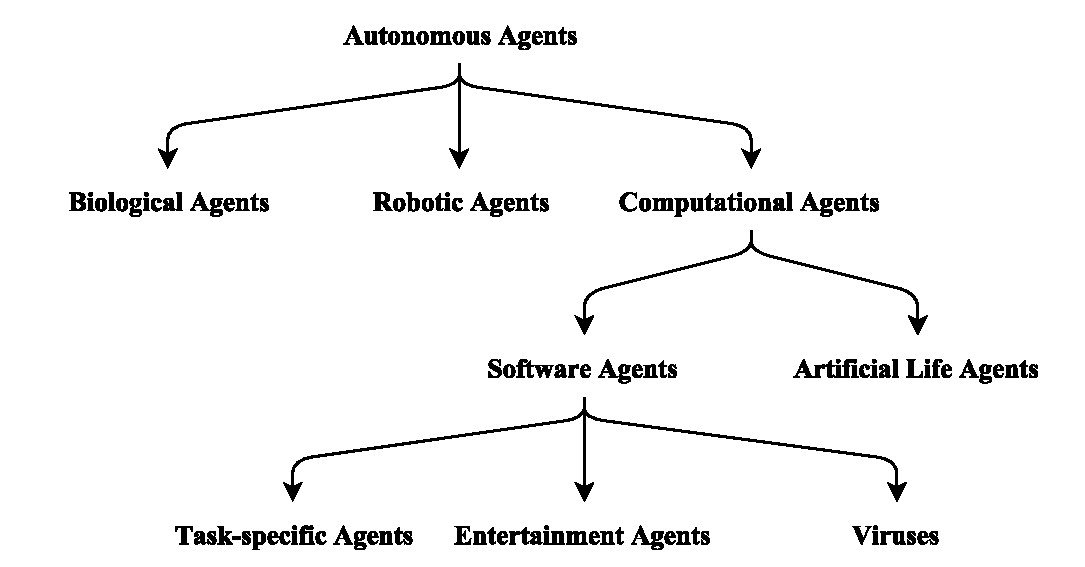
\includegraphics[max width=\linewidth,max height=8cm,keepaspectratio]{figures/franklinClassification}
    \caption{Natural Kinds Classification of Autonomous Agents in~\cite{franklin1996agent}}\label{fig:franklinClassification}
\end{figure}

Another division can be done by looking at the type of control mechanism: from rule-based systems that only follow handcrafted rules, to machine learning ones that learn dynamically from examples how to interact.

A very important characteristic to be considered when classifying conversational agents is the \textbf{initiative\footnote{ Jurafsky, D. (2017). Conversational Agents [PDF]. Retrieved from Stanford University course cs124 }}. With System Initiative only, the conversation is led by the bot and the user has only the possibility to say a finite set of things and cannot change directly the current state of the dialogue. It is the case when the user always replies to questions made by the bot, or when the only possibility of inputs is given by buttons. In dialogues between humans, the initiative usually shifts from one participant to another, and the same should apply in interactions with autonomous systems. For this reason, there exist mixed-initiative systems that try to take into consideration the user requests for tracking the dialogue state (and not imposing it).

Yet another division can be done by considering if the interaction scheme is single-turn (question followed by a response that only depends on the last question) or if the memory is required to perform a multi-turn dialogue. Multi-turn enables to refine searches and refer to entities previously mentioned, and are more natural than single-turn.

Other classifications that have been found are based on features such as believability and intelligence~\cite{isbister2002design}. Those features are reflected on how the user perceives the agent and are somehow similar to the goal of the imitation game: giving the illusion to talk to a person.

Given briefly those classification options, the choice has been to focus on two main dimensions for doing a classification: the first one (Section \ref{soaClassificationContents}) considers the contents of the dialogue, and is inspired by the objectives of Franklin et Graesser~\cite{franklin1996agent}. The second one (Section \ref{soaClassificationApproaches}) instead focuses on the approaches that are used.

\subsection{The information content}
\label{soaClassificationContents}

This first dimension considers the content of the conversation. Retaking the three objectives by Franklin et Graesser~\cite{franklin1996agent} (task-specific, entertainment, viruses) of autonomous software agents and removing the last one that is not inherent to conversational agents, the entertainment one is mapped to a generic chit-chat content (maintaining a general conversation with the user), while the task-specific one corresponds to domain specific knowledge (the bot provides it to the user acting as a natural language interface).

A third content type has been added to be able to categorize all those type of system that deal with different sources of information and combine them to provide rich answers. This may be called Encyclopedic Knowledge content, and the main ambition of those systems is to provide real answers to complex questions related to the world knowledge.

Those three main content types are explained in the following paragraphs, before going to discuss the existing approaches.

\subsubsection{Chit-chat}
The first type of content, that correspond to the native setting of the turing test because the goal is to entertain the user making him believe that the machine really understands the conversation, the history of chatbots is quite long.

The first chatbot ELIZA~\cite{weizenbaum1966eliza}, that was built in 1966, is of this kind. It was created mainly to demonstrate the superficiality of communications and the illusion to be understood by a system that is simply applying a set of pattern-matching rules and a substitution methodology.

ELIZA simulates a psychotherapist and, thanks to the trick of present again to the interlocutor some contents that have been previously mentioned, keeps the conversation without having an understanding of what really is said.\footnote{ ELIZA can be easily tested inside the text editor Emacs with the command doctor (meta-x doctor). } At the time when ELIZA came out, some people even attributed human-like feelings to the bot. A lot of other computer programs have been inspired by ELIZA. Even a markup language has been created to express the rules that drive the conversation (see AIML in \ref{aiml}).

A competition has been created to reward the progresses in this field: the Loebner Prize, an annual challenge that stands in the format of the Turing tests, but restricting the topics of conversation. Judges keep parallel conversations, one with a human and one with a computer program. Judges are chosen with the criterion that they $``$should respond naturally, as they would in a conversation with another person$"$ , in a way to avoid excessive sophistication. At the end the winner is the computer program that mostly convinced the judges (even without passing the Turing test). There are two more prizes in this competition: one is for the Turing test in text only interactions, the last one (the biggest one) is for passing the Turing test including visual and auditory inputs. This competition was first held in 1991, and with the years advancing the challenges have became more and more complex.

The Loebner Prize has been criticized by experts in the field because it rewards the usage of some tricks~\cite{shieber1994lessons}, pointing the focus on imitation instead of intelligence.

The commonly used tricks are~\cite{mauldin1994chatterbots}:

\begin{itemize}
	\item Let the conversation to be driven by the interlocutor. This works because most people like to talk about themselves and only want someone who listens;

	\item Give the illusion to be listening and understanding, by including substrings of the user input;

	\item Changing the topic when not understanding, that sometimes can be seen as paranoid;

	\item Simulated typing, delaying the responses.
\end{itemize}

The details of rule-based chatbots will be explained in more detail in \ref{soaRuleApproach}.

The evolution of chit-chat bots has recently evolved from a rule-based one to a generative approach. The key idea is to imitate existing conversations, and generate a response in a way that reflects both the training corpus and the current user turn (used as a stimulus). This approach, which will be discussed deeper in \ref{soaGenerativeApproach}, has its roots in using Statistical Machine Translation. The importance of the dialogue corpus, that dynamically establishes how the responses are generated, makes their availability a key element for a successful bot. For this reason these models are trained on few datasets publicly available: tweets, reddit discussions, ubuntu dialog corpus.

An example of this kind of systems is the mobile application Replika,\footnote{\url{https://replika.ai/}} that wants to provide a chat companion for its users. The conversation has no specific goals, and the system entertains the user with long discourses and games.

Focused on psychological support, an example of conversational system is Woebot.\footnote{\url{https://woebot.io/}} Entertaining the user with dialogues, it analyses the user mood and provides tips to feel better against depression and anxiety~\cite{fitzpatrick2017delivering}.

\subsubsection{Goal-oriented}
Another completely different type of bots is the one that provides a service on a restricted domain. It can be a natural language interface to a set of static Frequently Asked Questions, or can be linked to some dynamic content using some defined APIs. Those systems need to define the list of things they can do, and in some way map the user's requests to some actions.

Using those systems, the user should be aware of what the system can do and what cannot. Letting the user know that the bot he is interacting with can provide information only on the domain it is built for, should be a goal of the ideators. Responses for a little chit-chat conversation can also be added to the system, but they should be used only to avoid a general $``$\textit{I don't know}$"$  or $"$ \textit{I didn't understand}$"$ .

Those kind of bots can provide a more natural way of interacting with companies, both in the field of customer support and in search for information. The information can be statically defined as pairs of questions-answers. In this case the bot has to classify the user requests and provide the answer that mostly fits it. Or there can be some dynamic information that need to be extracted from the request. In this case, in addition to sentence classification, a parameter extraction needs to be performed. These tasks are the ones that this thesis will later focus on, and are the main part of the Natural Language Understanding process, which is described in \ref{soaNLUIntro} and analyzed in \ref{soaNLU}. The NLU approaches are quite handcrafted on the possible sentence types, and for this reason some more generative approaches are coming also in this field, inspired by the chit-chat domain. But what characterizes the conversational agents that provide this kind of content is the presence of a goal from the user: this is the reason that makes them called \textbf{goal oriented} agents.

\subsubsection{Knowledge-based}
As last type of chatbots, we can consider a richer version of the domain specific bot. Instead of limiting on a very restricted domain and predetermining the abilities with a static design of intents, this type of bots tries to provide a natural language interface towards a Knowledge Base. The fixed-structure intent based approach seems not to be optimal when the number of possible intents is very high and cannot be predetermined. If the system allows questions with a high level of complexity, requiring the linking of information, the number of intents quickly can explode.

Instead of doing a classification of sentences on some pre-defined intents, the goal of those systems is to transform the user sentence in a database query (for structured knowledge) or also to extract information from unstructured knowledge (such as documents expressed in natural language). This requires a strong relation between the Natural Language module and the Information Retrieval module. Structured knowledge can be composed of entities and relations between them. Information is in the form of RDF (Resource Description Framework) which have links to other entities with specific roles.

The sentences are analyzed using some parsers and are mapped to a set of linguistic patterns. After this translation (from human natural language to computer-understandable queries), the interrogation is performed using the content of a knowledge base. Those Question-Answering systems are actually very complex and involving different tasks and challenges~\cite{hoffner2017survey}.

A commonly used system that provides this kind of content is the Google Knowledge Graph, that explores the queries done on the search engine and provides linked information. Another example of them is the Wolfram Search, that can be asked questions like $``$\textit{who is the USA president?}$"$ . The focus here is not on managing complex dialogues, but understanding complex queries and exploring knowledge graphs.

There are however examples of encyclopedic knowledge systems that try to convey the conversational abilities of chit-chat dialogues empowering them with richer contents. This content ingestion is at the basis of the prototypes participating to the Alexa Prize.\footnote{\url{https://developer.amazon.com/alexaprize}} The goal that participants should try to achieve in this prize is to reach 20 minutes of dialogue with the user. Given a set of services (such as ASR, NLU, TTS), the teams have to design the dialogues and make it possible to carry on the conversation for the longest amount of time. Keeping such a long dialogue cannot be done by only providing simple responses using the tricks of ELIZA. Reasoning on topics requires having knowledge of them, so this kind of conversational agents are connected to knowledge bases.

\subsection{The approaches}
\label{soaClassificationApproaches}

The other dimension that is considered to make this classification is relative to the approach used. As will be seen shortly, bots require different stages (understanding, getting some information, answering) and different approaches can be applied to all of them.

As can be seen from the discussion on the content of the dialogue, there is an evolution of the approaches, leading to data-driven ones. The first wave of chatbot, as mentioned before, simply matched the input sentences with some keywords and responded in a way to make the conversation look natural. From this, a lot of other agents grew up with the same technique: pattern matching. With this approach, lots of bots have been built and even a specific markup language has been developed to express the patterns and link them to some responses.

More recent approaches instead tend to abandon the handcrafted rules towards an automatic learning from a dialogue corpus. This can be applied both to the part of natural language understanding (turn the user sentences into structured data) or also to the information retrieval and response generation.

We can do a classification of chatbot systems based on how much has to be specified and defined in a static way versus a dynamic approach that learns from the examples provided. This choice can be done in three main tasks: understanding, information retrieval, response generation. Each of them can have three levels of dynamicity: the first one is completely rule-based, the second one is mixed, usually presenting a dynamic categorization over pre-defined types, while the third one is completely dynamic. In the following Table~\ref{tab:approachCombination}, the levels are shown for each task.

% !TEX encoding = utf8
% !TEX root = ../main.tex

\begin{table}
  \begin{tabularx}{\textwidth}{rLLL}
    \toprule
    \textbf{Dinamicity level} & \textbf{Understanding} & \textbf{Information retrieval} & \textbf{Response generation} \\
    \midrule
    0 & Pattern based (entities and intents) & None / Fixed data & Rule-based template \\
    \midrule
    1 & Machine Learning (entities and intents) & Fixed API & Dynamic template: retrieval based \\
    \midrule
    2 & Encoding (sentence embeddings) & Dynamic exploration & Generative \\
    \bottomrule
  \end{tabularx}
  \caption{The different approaches to Understanding, Information Retrieval and Response Generation}\label{tab:approachCombination}
\end{table}

The understanding task is the one related to turning the natural language sentences into something that can be understood by the machine: its output can be a pattern match for level 0, structured data for level 1 (NLU) or an encoded representation for level 2. 

The information retrieval task instead, if present, can use a fixed set of APIs or be more dynamic, interacting with information and their relations (graph knowledge bases).

Instead the response generation can be fully governed by handcrafted rules (e.g. if a set of conditions apply, say that). Or decide the template response from a finite set using statistical approaches (using some proximity measures like \textit{TF-IDF}, \textit{Word2Vec}, \textit{Skip-Thoughts}). Or being generative, with responses that are built on the fly by a seq2seq model.

\begin{figure}[!htbp]
    \centering
    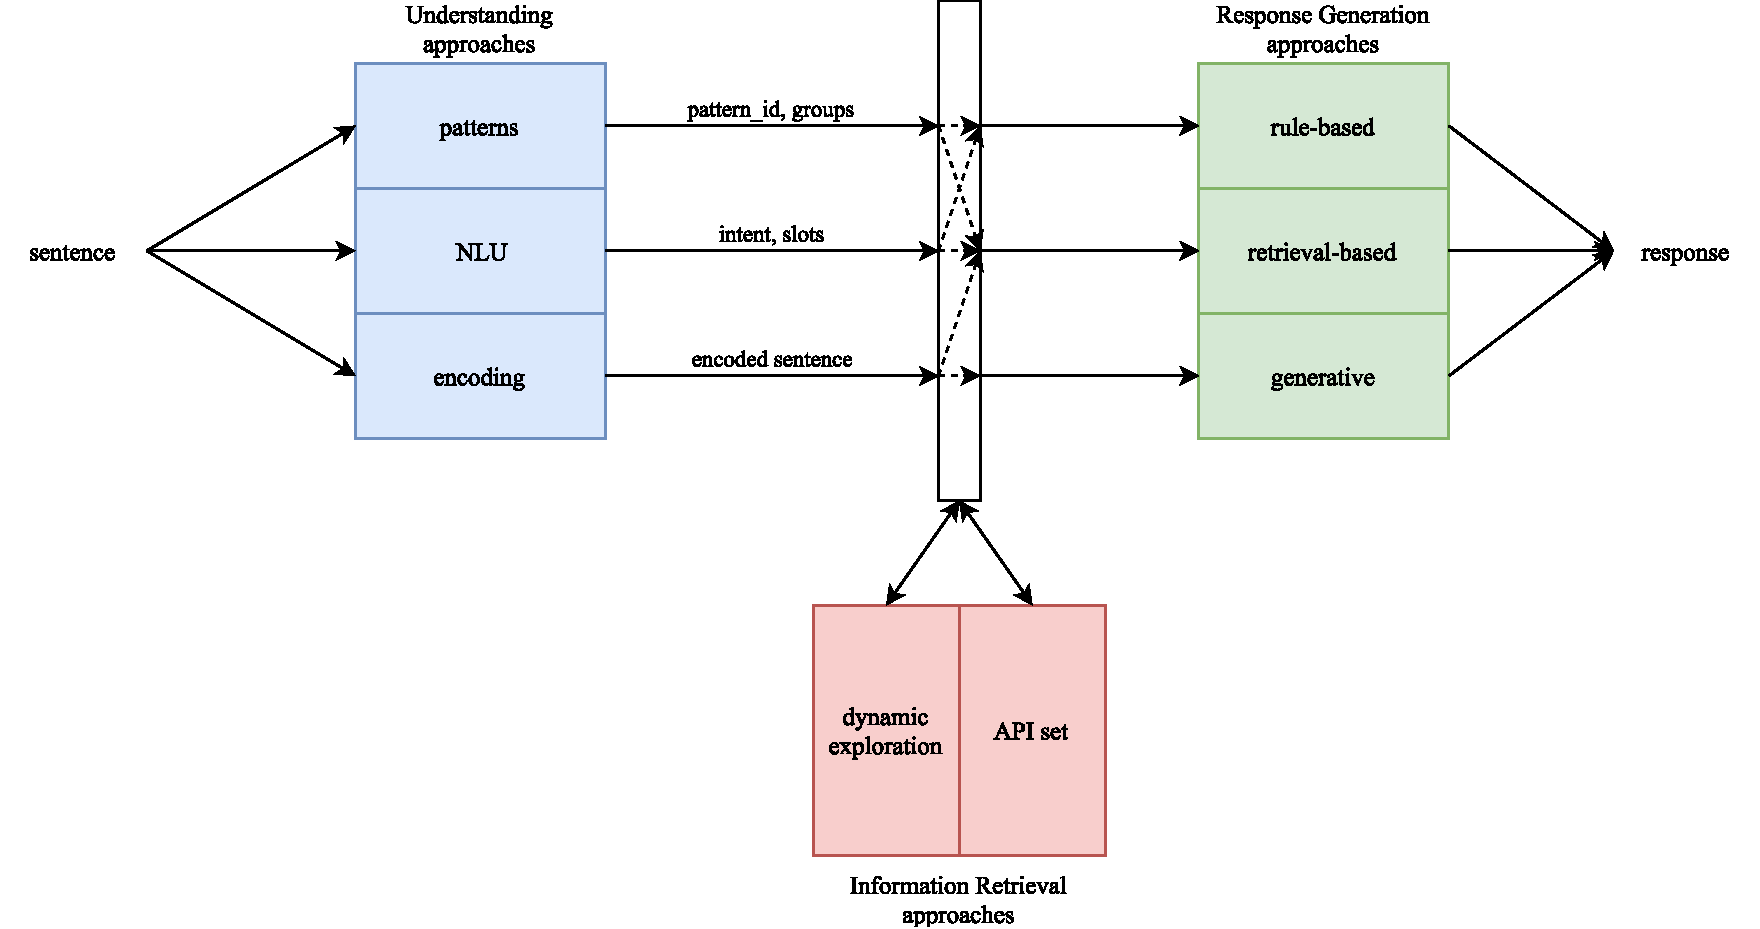
\includegraphics[max width=\linewidth,max height=8cm,keepaspectratio]{figures/approachesCombination}
    \caption{How the approaches for each task can be connected together}\label{fig:approachesCombination}
\end{figure}

The choices are not independent however, as can be seen from Figure~\ref{fig:approachesCombination}: since the tasks are put in a chain (first understanding, then retrieving the information and ultimately formulating a response), the approach chosen on the first stages has consequences on the following ones. Choosing to use ML instead of dynamic understanding precludes the possibility to have generative responses, because the user utterances will be categorized on a finite set of types (intent types) unless a hybrid understanding is performed (NLU to find the intent types with a parallel sequence-to-sequence model for chit-chat dialogues). For this reason and being the understanding stage the first one, the details on the approaches will be analyzed mainly on this first task, and for each level in it some details will be given on the possibilities for the other two choices.

The choice between those possibilities has to be done based on the available data (e.g. if transcripts of existing human conversations exist), and on the main information content the system will provide (see above, between chit-chat, domain-specific, knowledge-based) because the approach performance depend a lot on it. It is also necessary to keep in mind that complex dialogues actually can perform better if at dialog management level an handcrafted approach is kept. ML can help reconduct on sentence types, but actually structured topic dialogues need handcrafting. As of today, deductive (from rules) decision-taking in conversation gives better performances with respect to inductive (only learning from examples), because it gives more control to the designers of dialogues.\footnote{\url{https://developer.amazon.com/alexaprize}}

Moving the level of dynamicity higher, the \textbf{complexity} moves from handcrafting very specific features, that can be very specific to the domain of application and therefore provides a solution that difficulty can be ported to new domains, to the complexity of the approach itself. The transition usually is towards approaches that involve machine learning techniques like neural networks: the engineering of those networks is quite complex with respect to writing patterns to cover a set of sentences. In addition, also more computing power is required to run those heavy systems.

Changing the selected approach (especially on the understanding and generation processes) also has consequences on the additional work that has to be done to port the agent to \textbf{other languages}. A rule-based understanding is highly coupled with the used language. Using NLU reduces a lot this dependence because instead of manually deciding how to categorize the sentences, the system will find automatically how to do that even in another language, if the appropriate annotated training examples are provided and if the network structure itself is sufficiently language independent. As will be described in the NLU chapter, using features of words that are more related to their meaning (contextual and semantic, following the $``$distributional semantics$"$  concept) instead of their grammatical role, helps generalizing and being less dependent on the selected language (see usage of word embeddings and how they can be easily generated for any language).

Summing up, a more dynamic, end-to-end approach has an higher complexity but leads to easily adaptable solutions, in terms of new domains and new languages.

\subsubsection{Rule-based}
\label{soaRuleApproach}

This approach has both the understanding part and the response generation specified as rules. It was firstly used for chit-chat systems, and the number of rules can be quite big. Those rules can define theirself a response or can refer to other rules in order to reduce the amount of different actions. However this strategy is not very good because a lot of rules must be written in order to span all the possible variations of sentences. Moreover, since the majority of the work is to write those rules, and the rules highly depend on the language analyzed, this approach can hardly be applied on different languages and the process of migration from one to another requires the rewriting of the whole set of rules.

Chit-chat systems historically do not use knowledge bases to provide responses. The information that they provide is statically written as part of the  system background.

This approach was firstly used by ELIZA~\cite{weizenbaum1966eliza}. Then, when used by ALICE, an extended version of ELIZA, there has been the release of AIML, that is the markup language used for expressing the rules. With the release of AIML, lots of implementations of chatbots used this approach.

\label{aiml}

\textbf{AIML} stands for Artificial Intelligence Markup Language and is a language that describes how the bot replies to certain inputs. Inputs are evaluated against a set of patterns and the best matching (category) is chosen. The actions performed by the category can be a simple response or can also set the values of state variables and invoke other categories. Those rules determine together the classification of the sentences and the response generation.

A rule (in the AIML jargon is called category) is made up of a pattern and a template. As can be seen in~\ref{fig:aimlExample}, the pattern is responsible to identify the sentences that activate the rule, while the template is the part that manages the response: a template can be both a sentence that will be sent to the user or can be a redirection towards another rule (\textit{srai} rules). In addition to those two elements, some actions to manage the state of the conversation can be added: variables can be set and read to to conditionally activate rules.

\begin{figure}[!htbp]
    \centering
    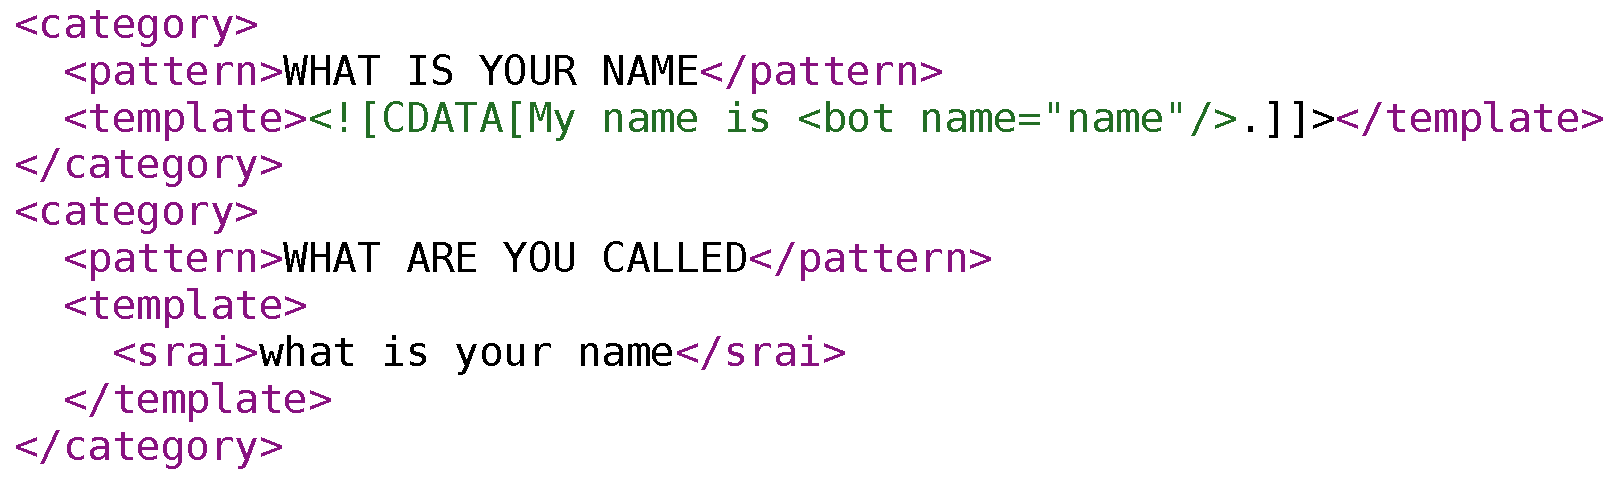
\includegraphics[max width=\linewidth,max height=8cm,keepaspectratio]{figures/aimlExample}
    \caption{An example of the rule-based AIML}\label{fig:aimlExample}
\end{figure}

While writing those rules can be quite easy, the problem is that a lot of them must be written to manage the variations on the natural language. In fact, the strategy used for managing the development cycle of bots empowered by AIML is a cyclical process: starting with a model with some rules, the system is tested against a group of test users collecting the interactions; at the end of the test session, the logs are analyzed and the developers modify and add rules to provide suitable responses. This process is called \textbf{targeting}. The developer role can be separated from the role of tester or testers can be given privileges to modify the rules on their own.

The disadvantages of using AIML are many. First of all, being a rule based system, a big set of rules need to be built and so a big fraction of time is spent analyzing the possible variation of the sentences instead of leaving it for more important tasks such as focusing on the data available. A lot of rules are also needed to perform reduction on other rules. Those additional rules make very difficult to understand what is wrong when multiple reduction rules have been applied. Other problems come when the sentences contain complex queries. In this situation, it is possible that more parameters need to be extracted from a single sentence, and since every pattern can contain a maximum of one wild character some tricks must be used.

AIML is used on bots based on ALICE. Being the markup language released under GNU GPL license, a lot of open source tools exist, only requiring the developers to produce a set of AIML rules. Even online services exist that can be used to deploy an AIML bot in very few steps (for example pandorabots\footnote{\url{https://home.pandorabots.com/en/}}).

Also considering that AIML was born for generic chit-chat systems and the Loebner Prize, it has been used also in domain specific bots. For example, to provide answers to Frequently Asked Questions in the domain of student support in Universities~\cite{ghose2013toward}. The information contained in the FAQ are relative to admissions and courses information. The AIML rules for managing conversations on these topics have been added to a base ALICE bot, and a change in the state transition management has been done in order to make the conversation stay on the desired topics, using weighted transitions that make the bot prefer to stay on the university domain. This system has been tested on students, establishing some evaluations on their satisfaction and also on the topic switching rate, in order to have some measures on the state transition management.

Other examples of rule-based systems are bots that manage the interaction with the user by only providing \textbf{buttons}. In this way, the dialogue is completely managed by the bot and the interlocutor can only decide on a finite set of choices at every turn. This is a very unnatural dialogue scheme, where the initiative belongs completely to the bot. A lot of bots today belong to this category, because in this way the dialogues are strongly reliable and the state of conversation can be tracked and managed easily without unexpected utterances. About the information retrieval, those bots usually interact with a fixed set of APIs (as most domain-specific bots do).

\subsubsection{NLU}
\label{soaNLUIntro}

Another approach that can be used for the understanding task, instead of manually matching sentences with patterns, is to have a Natural Language Understanding engine that performs this classification in a smarter way. In this approach, instead of building rules and analyzing the structure of the sentence in order to span the different variation of sentences that should be grouped together, the objective is to have a classifier that can be trained to make this task automatically using machine learning techniques (feeding training examples, letting the internal parameters to be adjusted automatically to obtain the desired outputs).

Natural Language Understanding applies only to the task of understanding the sentences (turn natural language sentences into structured data), and not to the response generation. NLU is composed of two subtasks: sentence classification, also called intent detection, that finds for each input sentence a predetermined type that expresses what the user wants to communicate or ask; slot filling, also called entity extraction, that is responsible to obtain from sentences some parameters that have been previously defined in their type.

This approach is born for domain specific bots and responds to a problem that is inborn to this kind of bots: exists a big difference between the natural language and the information with fixed structure stored in knowledge bases. Using Natural Language Understanding techniques, an intermediate representation can be built starting from the sentences in natural language and from this representation, composed of intent and entities, it is easier to interface with the fixed structure information that are usually reachable using some statically defined APIs (information retrieval) and also manage the state of the dialogue, recording which intents and entities have occurred (dialogue manager).

NLU can also be used when the dialogue manager is not statically defined, but is trained to provide the correct responses and call the right APIs over a predefined set. In this solution, there are not rules defining how to track the state of the conversation, because they are inferred from the training corpus. This technique, for example, is used by the open source company RASA,\footnote{\url{https://rasa.ai/products/rasa-core/}} that provides a model that not only takes care of NLU (handling intents and entities), but also can manage a dynamic state tracking. Based on a fixed set of patterns provided by the developer and actions (that may call external APIs), the state tracker can be trained both by providing dialogue examples or by doing online learning (asking for feedback after every turn) for a quick annotation of new corpora.

\subsubsection{Encoder-Generative models}
\label{soaGenerativeApproach}

Going further with automation techniques that learn from examples, if the management of the state of the dialogue and the information retrieval and the response generation are managed without writing static rules, the approach is said to be generative. Using this approach removes the intermediate point of contact between natural language and rule-based systems that is used in NLU systems. Everything is trained together in a end-to-end fashion: from the input sentences to the output sentences.

This approach was born in the chit-chat domain and has its strength when combined with a huge corpus of dialogues. Given the dialogues, which are sequences of sentences said by different actors, the system is trained to generate the next sentence given the current dialogue history.

The first implementation of this strategy was trained on tweets~\cite{ritter2011data}, but other works have been trained on Ubuntu Dialogue Corpus~\cite{lowe2015ubuntu} and many other datasets.

The technology used is the one that is used to provide translations, with some modifications. The model for the generation is trained on the corpus and learns how to generate the next sentence from the previous ones with an encoder-decoder structure. This structure, as will be seen applied for slot tagging in \ref{soaSeq2Seq}, uses LSTM cells, that can capture features of sequences adaptively using the memory capabilities of their recurrent nature. The encoder network (can be seen as the understanding part) collects the useful features while the decoder, given an initial state from the encoder and given a stimulus, begins the generation of the new sentence and stops when appropriate.

A even more complex approach is the one described in~\cite{serban2016building} that uses a hierarchical RNN: the lower level is applied on words, both in the encoder and the decoder, while a coarse-grained RNN applied on the sentences is used to model the topic propagation over the turns.

The main advantage of this kind of approach is that responses are generated completely in automatic way and thanks to LSTM cells can contain elements that were previously mentioned in the conversation. Being generative, they always produce an output even when the inputs are very different to the ones used in the training phase. This can be seen as good generalization ability, but can result in the generation of unpredictable and strange sentences, even when huge corpora are used for training. Grammatical errors can also be generated in the output sentences if no post processing checks are done.

To overcome those problems, reinforcement learning strategies can be applied, in order to learn in an online setting also from the dialogues that occur at runtime. This is a good strategy in general, but it can lead to some unwanted effects of polarity of the responses if there is not a supervision: the example of Microsoft Tay, that after 16 hours on Twitter was shut down because of the offensive tweets that was generating.\footnote{\url{https://www.washingtonpost.com/news/the-intersect/wp/2016/03/24/the-internet-turned-tay-microsofts-fun-millennial-ai-bot-into-a-genocidal-maniac/}}

Having a model trained on a wide variety of dialogues also rises the problem of the coherence of the responses: it is easy that, without filtering and post-processing the responses, the bot replies in different ways to questions inherent to the same topic. For this reason a persona-based model can be built in order to consider also some more inputs to the generator of the responses, that can model some features of the speaker, such as background information and speaking style~\cite{li2016persona}. Those features can be encoded into distributed embeddings and be provided to the generator both in the training and in the inference time.

Another common problem of this approach is that it tends to generate commonplace responses, because it is trained to maximize the likelihood of the output for the given input. It is like providing an average response that fits the current input. A proposed solution to reduce this effect is to use Maximum Mutual Information as objective function in the neural model. This will try $``$\textit{to take into account not only the dependency of responses on messages, but also the inverse, the likelihood that a message will be provided to a given response}$"$~\cite{li2015diversity}. Using this solution, a clear decrease in the proportion of generic responses can be observed on the outputs.

This generative approach has shown good results for non-specific task dialogues, because the goal is simply to continue the dialogue and there is no need to introduce some task-specific information.

As an example of this approach in action, Google Smart Reply applies it to generate short email responses that can selected and completed. The implementation takes in account the incoming email to generate responses that may be used to replay~\cite{kannan2016smart}.

In the field of domain specific bots, usually the responses are not generated completely from sequence-to-sequence models. The approaches usually make use of templates that can be chosen by rules or by a dynamic classifier. But in some way templates are always used to provide the answers to domain-specific questions.

The dynamism can also reach higher levels on the information retrieval task, without requiring fixed APIs but allowing simple key-value data storage to be queried in natural language: this approach has been proposed by Eric and Mannings~\cite{eric2017key}.

\subsection{The challenges}
\label{soaChallenges}

For the different contents and approaches that have been analyzed, different challenges arise with bots that should provide some kind of valuable content.

The most important point is to classify the user sentences and to reconduct them to a set of questions that have a response by design. This challenge of \textbf{understanding} the user is made up of two components: one is relative to the natural language understanding of the current sentence, while the other one is relative to the contextualization of the current sentence in the environment of the dialogue. While talking, humans tend to refer to previously mentioned things, and the understanding of sentences is often difficult without placing it into its \textbf{context}. Some approaches to solve this problem are explained in the section \ref{soaInteractionContext}, explaining the concept of multi-turn and dialogue tracking.

Another challenge that arises, especially on generative approaches, is the \textbf{coherence} of the sentences that are said. Since the training of those models is done on dialogues between multiple users with different visions and different behaviour, it may be difficult to establish a coherent personality of the bot. This issue is not present if the approach chosen makes the response generation in a static way: in this case it is sufficient to keep a coherent personality among the people writing the response templates.

Another big issue is how to deal with \textbf{unexpected questions}, for which a response has not been prepared. This problem is present in rule-based approaches, in NLU-based bots and even in generative approaches.

The next section will investigate the Natural Language techniques that are used for domain specific bots, focusing on the tasks of intent recognition \ref{soaIntent} and slot filling \ref{soaSeq2Seq} and how to manage a dialogue in a multi-turn environment \ref{soaInteractionContext}.

\section{Natural Language Understanding}
\label{soaNLU}

As introduced previously, NLU is the process of turning sentences into structured information. Two asks are involved:intent classification and slot filling. Usually those tasks are performed in statistical way, not applying a static set of rules as was done with AIML and similars. Natural Language Understanding belongs to the Natural Language Processing (NLP) family whose components are involved in text processing in very different ways.

Starting from the easiest NLP component, tokenizers are part of this family. The role of a tokenizer is to split texts into tokens that correspond to words and also punctuation (if punctuation is relevant for the current problem, or can be removed by the tokenizer).

Other important components of NLP are Part-Of-Speech recognizer and Dependency Parser, that are responsible to parse (this term is also used when elaborating source code; some approaches can be taken from source code parsing, but usually the natural language grammar is more complex and ambiguous and is better analyzed by statistical parsing~\cite{ballesteros2015improved}) the sentence and individuate the grammatical roles of the words.

Another commonly used component of NLP is the Lemmatizer: its role is to reconduct to the base form all the words that derive from others. This is used to reduce the cardinality of vocabularies and simplify some tasks, for example finding the topic of the conversation.

Another thing that is done using NLP is Named Entity Recognition: this finds occurrences in the text of some entities that belong to some types: common types are Person, Organization, Country, Location, Date, Time, Numbers, Currencies. This component usually mixes an approach based on POS combining them with a knowledge base that enumerates in some way what belongs to each entity type. The Slot Filling task is quite similar to NER, and the differences will be analyzed soon. The NER can have some complications when the talker refers to previously mentioned entities by using explicit signs (such as pronouns or definite nominals) or implicit references (such as ellipsis): this is the non trivial problem of \textit{coreference resolution}, that is analyzed in \ref{soaCoreference}.

Other components are more focused on the sentence as a whole: Sentiment Analysis that tells if a sentence is positive negative or neutral, Summarization, Sentence Classification to find topic or complexity level for example. The intent detection task can be put in this last group.

For this work we are interested mainly in two very specific tasks (intent classification and slot filling that are described soon) that usually are denoted by the Natural Language Understanding label. The other NLP tasks (syntactical analysis, POS tagging) are not main interests here, however some of them, such as sentiment analysis, can be used to detect the mood of the writer, as will be discussed in the personalization section \ref{soaPersonalization}.

\subsection{Goals}
As mentioned before, from the sentences NLU wants to:

\begin{itemize}
	\item Classify the intent (what the user wants, against a set of predefined ones);

	\item Extract the entities mentioned (we may want to care about only a specific set of entity types that are relevant to the abilities of the bot). This task is somewhere called slot filling, because the words that we want to extract may also not be entities. $``$The slot filling task is to search a document collection to fill in values for predefined slots (attributes) for a given entity.$"$  Furthermore, slots in a sentence can be designed to have a role (in order to be able to discriminate between multiple instances of the same type of entity). This feature is not present in the Named Entity Recognition task because the objective is only to recognize the entities, not to give them a role as a parameter in a programming language. For this reason the name of this task can be both $``$slot filling$"$  and $``$entity extraction$"$  with preference for the first one that gives more the idea of roles, while $``$named entity recognition$"$  is quite unappropriate.
\end{itemize}

For example, for the sentence $``$is Turin a supported city?$"$  we may want to categorize it as a question that asks if a city is supported (this is the intent) and extract the word $``$\textit{Torino}$"$  that is the city the user is looking for (this is a slot that corresponds to an entity of type CITY or simply LOCATION depending on the granularity of entities defined).

The first task corresponds to a classification of the user sentences to decide what is the intention of the user. Since a bot is usually designed to answer to different types of questions, this stage is responsible for finding the type of question. The slot filling task instead is a process that annotates some parts of the input sentences with the name of the corresponding slot. A slot can be thought as a field in an online form. While the intent represents the type of question, the slots of a sentence are values that the bot must be able to extract from the sentences because they are used as parameters for the application logic.

For both the goals, different approaches are described in dedicated subsections: the intent classification related ones are analyzed in \ref{soaIntent} while the slot filling ones in \ref{soaSeq2Seq}.

Once the intent and the slots have been analyzed on the current sentence, we can have some rules at the application level that can put some constraints. For example, for a certain type of question, one or more slots can be compulsory. In this case, the conversation should make the user provides the values by prompting him some questions. These types of constraint make the interaction model more complex and require an analysis over multiple user and machine turns, as will be seen in Section \ref{soaInteractionContext}.

The two tasks can be done independently, but some recent studies (like~\cite{guo2014joint} and~\cite{liu2016attention}) have shown that there can be benefits if they are performed together.

\subsection{Recurrent Neural Networks}
This section contains a description of the different structures of neural networks that have reached the State of the Art condition and have been described in literature.

A neural network approach can be used for the tasks of slot filling and intent detection. The first thing that needs to be done is to point out what are the inputs and outputs of the system. Once defined the inputs and outputs, we can think of a component that implements the desired functionalities. The inputs to the network are the words contained in the sentence and the outputs are the intent label (for the intent classification task) and the slot labels (for the slot filling task).

As slot labels, the slot names can be used directly but, in order to better handle multi-word slots, a commonly used format is the IOB introduced in~\cite{ramshaw1999text}, where the O indicates $``$other$"$ , the B is the beginning of a slot and the I is the label associated with a word that continues the slot of the previous word. The IOB labels are prepended to the slot name.

An example of inputs and expected outputs, showing the IOB annotation scheme, is represented in Figure~\ref{fig:iob}.

\begin{figure}[!htbp]
    \centering
    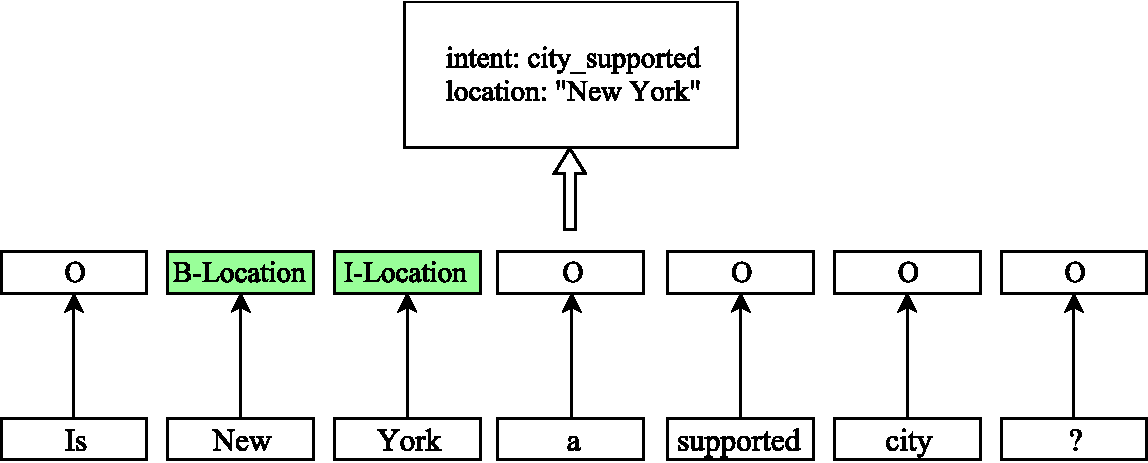
\includegraphics[max width=\linewidth,max height=8cm,keepaspectratio]{figures/iob}
    \caption{The Inside Out Beginning annotation scheme}\label{fig:iob}
\end{figure}

Instead of using simple feed-forward networks, a lot of studies make use of networks with recurrent components. The core idea behind RNN is to make use of sequential information. In feed-forward networks, the assumption is that each input-output pair is independent from the others. For RNN, the recurrence stays in performing the same task for every element of the sequence, making the output depending on the previous steps. This idea can be seen as the RNN having memory that keeps information from the past iterations. Specifically on the ability of remember and use in the correct way their memory, a lot of studies have been done to develop particular cells (a cell is the basic building block for RNNs).

\begin{figure}[!htbp]
    \centering
    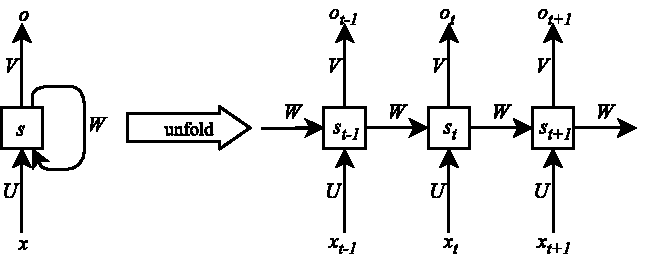
\includegraphics[max width=\linewidth,max height=8cm,keepaspectratio]{figures/rnnUnfold}
    \caption{The temporal unfolding operation on a simple RNN structure}\label{fig:rnnUnfold}
\end{figure}

A recurrent cell is a type of cell that takes as input also its previous output. Those types of neural networks have been designed for problems where the order of inputs matters, and the length of input sequence can vary. For example, they are commonly used with sequence of words, characters, frames in a video and their goodness stands in modeling features that belong to the sequence. Unlike feed-forward nets, that consider the fixed set of inputs to generate the outputs, the recurrent nets are applied in different timesteps to elements belonging to a sequence and, thanks to the loops of their cells, retain information from previous timesteps and the output depends on them too.

Since the same network (and cells) are used in different timesteps, the analysis of RNN is usually performed on the unfolded version of the network (see Figure~\ref{fig:rnnUnfold}): the single elements are repeated different times (one for each timestep) and the looping links are now going from the element in the previous time to the next time. In this way, a recurrent network is transformed into a multi-layer feedforward network, but keeping the same weights on the unfolded elements that generate from the same recurrent cell.

The unfolding operation sometimes is also called unrolling because of the similarity to the loop unrolling.\footnote{\url{https://en.wikipedia.org/wiki/Loop\_unrolling}}

\subsubsection{Backpropagation}
Backpropagation is the algorithm used in neural networks to update the weights, that is used also for the training of recurrent networks, with a slight modification.

The goal of the backpropagation training algorithm is to modify the weights of a neural network in order to minimize the error of the network outputs compared to some expected output in response to corresponding inputs. It is a supervised learning algorithm that allows the network to be corrected with regard to the specific errors made.

The general algorithm is as follows:

\begin{itemize}
	\item Present a training input pattern and propagate it through the network to get an output;

	\item Compare the predicted outputs to the expected outputs and calculate the error;

	\item Calculate the derivatives of the error with respect to the network weights;

	\item Adjust the weights to minimize the error;

	\item Repeat with other training samples.
\end{itemize}

In this way the Neural Network, which is a combination of layers with tunable parameters, learns to predict the expected output of the training samples. The goodness of the network is to obtain correct outputs also for reasonably similar samples that were not seen in training time.

With RNNs the training mode is very similar. The name of the modified algorithm is BackPropagation Through Time (BPTT)~\cite{werbos1990backpropagation} and is basically the standard algorithm applied on the temporally-unfolded version of the network. The only difference is that, since the layers correspond to different timesteps of the same cell, the weight updates in each instance are summed together. In other words, the temporally-unfolded neural network is a deep neural network with shared weights.\footnote{\url{http://www.wildml.com/2015/10/recurrent-neural-networks-tutorial-part-3-backpropagation-through-time-and-vanishing-gradients/}}

As can be see in Figure~\ref{fig:bptt}, the loss function in backpropagation for each observed error (the difference between the true value and the predicted one, denoted with  \( E \) ) affects the current and previous timesteps with partial derivatives. For example, if we want to consider the gradient of the error  \( E_{2} \) with respect to the inputs  \( x_{2} \) ,  \( x_{1} \) and  \( x_{0} \)  we can apply the chain rule:

 \(  \frac{ \partial E_{2}}{ \partial x_{2}}=\frac{ \partial E_{2}}{ \partial s_{2}}\cdot \frac{ \partial s_{2}}{ \partial x_{2}} \) 

 \(  \frac{ \partial E_{2}}{ \partial x_{1}}=\frac{ \partial E_{2}}{ \partial s_{2}}\cdot \frac{ \partial s_{2}}{ \partial s_{1}}\cdot \frac{ \partial s_{1}}{ \partial x_{1}} \) 

 \(  \frac{ \partial E_{2}}{ \partial x_{0}}=\frac{ \partial E_{2}}{ \partial s_{2}}\cdot \frac{ \partial s_{2}}{ \partial s_{1}}\cdot \frac{ \partial s_{1}}{ \partial s_{0}}\cdot \frac{ \partial s_{0}}{ \partial x_{0}} \) 

\begin{figure}[!htbp]
    \centering
    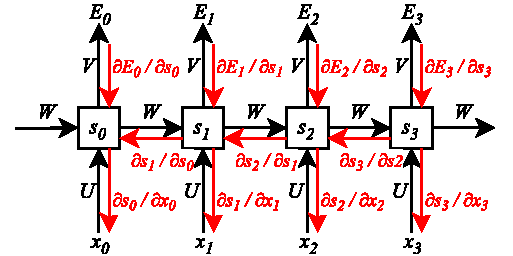
\includegraphics[max width=\linewidth,max height=8cm,keepaspectratio]{figures/bptt}
    \caption{The Backpropagation Through Time: how the errors are propagated}\label{fig:bptt}
\end{figure}

\subsection{Cell types}
This paragraph describes the  cell types used in this thesis. Such cells are the basic units used for the network architectures explained successively. As a layer in feedforward NN is composed of neurons, a layer in a RNN is composed of a recurrent cell. The cell holds the matrix parameters to compute outputs and next state given the current state and current input.

\subsubsection{Simple RNN}
The simplest recurrent cell type is a block with two inputs and two outputs. As can be seen in Figure~\ref{fig:simpleRNN}, one input is the actual input at the current timestep while the other one comes from the previous timestep (or from initialization on the first time). The cell produces an output ( \( y_{t} \) ) that can be passed to the next layers of computation (recurrent or not) or be used as a probability distribution passing through a \textit{softmax}. For the next timestep the cell also produces the current state ( \( h_{t} \) ) that is used on the looping connection; the state has the same value as the output, and the different name is given only to to put the emphasis on the different destinations for each one of them.

\begin{figure}[!htbp]
    \centering
    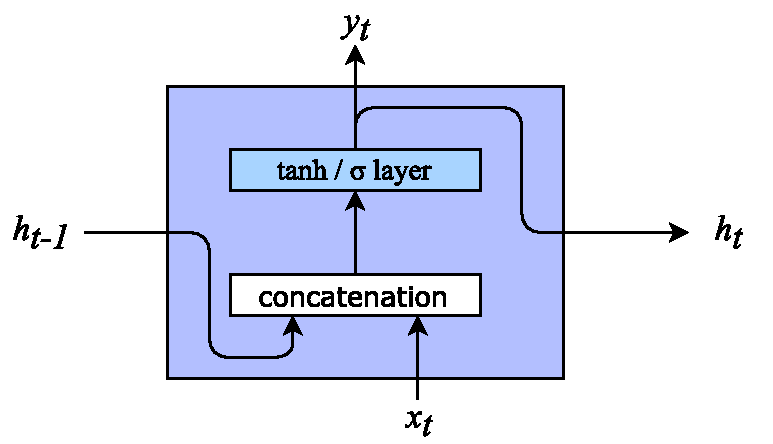
\includegraphics[max width=\linewidth,max height=8cm,keepaspectratio]{figures/simpleRNN}
    \caption{A simple RNN with a single layer inside}\label{fig:simpleRNN}
\end{figure}

The two inputs are concatenated and passed through a single feed-forward layer that corresponds to a linear transformation plus a non-linear function (e.g.  \( tanh \) ,  \(  \sigma  \) ). The next state is computed as  \( h_{t}=tanh \left( W\cdot  \left[ h_{t-1}, x_{t} \right]  + b \right)  \)  where the notation of square brackets denotes the concatenation operation, and  \( W \)  and  \( b \)  are respectively weights and biases.

Since the same cell is applied many times in time, and the recurrence loop feeds back the output as inputs, there can be easily two kinds of problem due to the fact that the weight matrix coefficients are multiplied at each timestep:

\begin{itemize}
	\item Exploding gradient: if some coefficients are greater than 1, the output values can become soon very big, making the network insensible to new inputs because is in some way saturated. The solution to this problem is using some non-linear function that limits the values not to be over the value of 1;

	\item Vanishing gradient: if some coefficients are near to 0, the network will quickly forget previous inputs and the output will not depend on them.
\end{itemize}

This can also be seen in the formulation of BPTT. There are two factors that can affect the magnitude of gradients - the weights and the activation functions (or more precisely, their derivatives) that the gradient passes through. If either of these factors is smaller than 1, then the gradients may vanish in time; if larger than 1, then explosion might happen. For example, the  \( tanh \)  derivative is smaller than 1 for all inputs except 0; sigmoid  \(  \sigma  \)  has even lower values because it is always less than  \( 0.25 \) .

Those problems have the same origin: the simple RNN is not able to manage long-term dependencies. This problem has been analyzed in detail by~\cite{bengio1994learning},~\cite{hochreiter1998vanishing} and other types of cells have been proposed.

\subsubsection{LSTM}
LSTM~\cite{hochreiter1997long} is a solution that came out in 1997 in which a more complex cell is considered. The main idea is to have some gates that decide how much of the previous cell state to keep, and how much of the current input to consider for the calculation of the current state and current output.

\begin{figure}[!htbp]
    \centering
    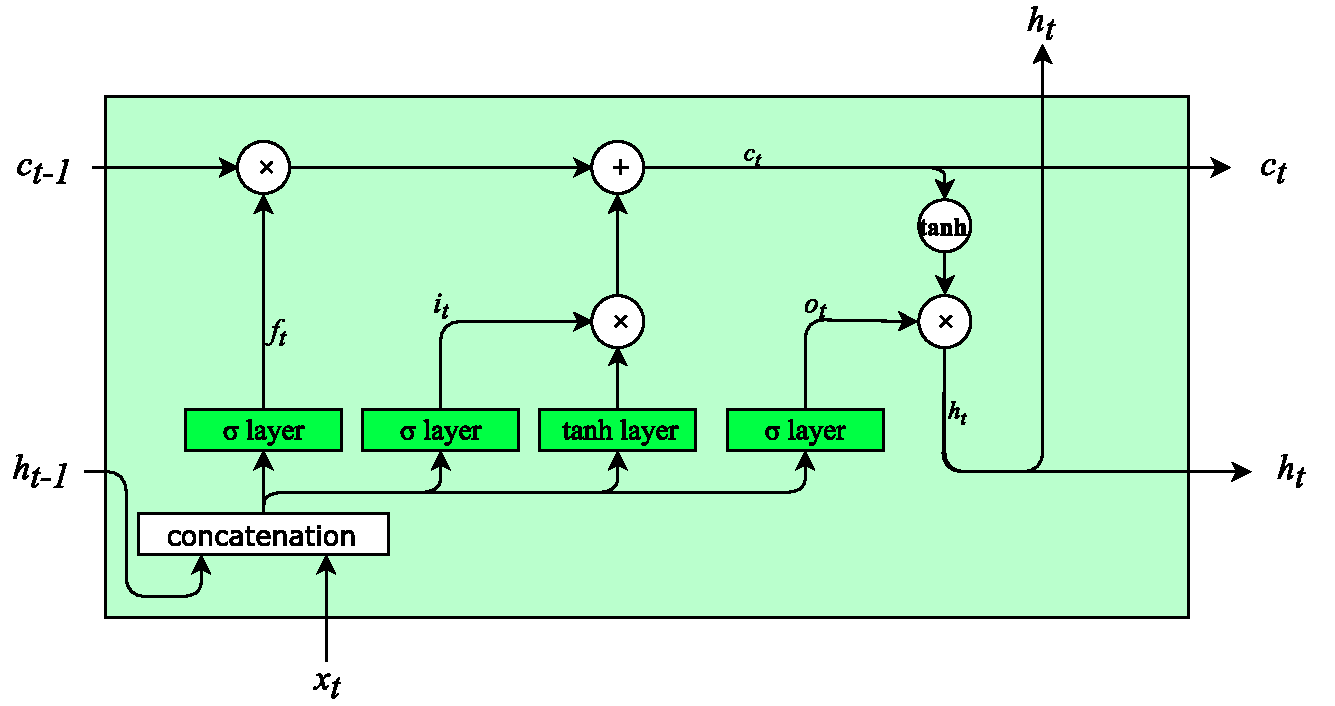
\includegraphics[max width=\linewidth,max height=8cm,keepaspectratio]{figures/LSTM}
    \caption{The Long Short-Term Memory cell proposed in~\cite{hochreiter1997long}}\label{fig:LSTM}
\end{figure}

In addition to the simple RNN cell, we can see in Figure~\ref{fig:LSTM} that three more \textit{gates} are added:

\begin{itemize}
	\item Forget gate  \( f_{t} \) :\ decides how much of the previous hidden state to keep.   \( f_{t}=tanh \left( W_{f}\cdot  \left[ h_{t-1}, x_{t} \right]  + b_{f} \right)  \) 

	\item Input gate  \( i_{t} \) : decides how much of the current input to consider.  \( i_{t}=tanh \left( W_{i}\cdot  \left[ h_{t-1}, x_{t} \right]  + b_{i} \right)  \) 

	\item Output gate  \( o_{t} \) : decides how much of the hidden state is exposed to the output.  \( o_{t}=tanh \left( W_{o}\cdot  \left[ h_{t-1}, x_{t} \right]  + b_{o} \right)  \) 
\end{itemize}

All those gates are implemented with single layer feedforward networks. This type of RNN is able to manage better the long-term dependencies, at the expenses of having four times the parameters. But with sufficient training examples, the network is able to learn how to output the correct values and how to mix the different inputs.

Many implementation\ exist of this cell, the most common is the basic LSTM that is shown in  Figure~\ref{fig:LSTM}, but variations exist (with peephole connections, or other variations on the gates\footnote{\url{http://colah.github.io/posts/2015-08-Understanding-LSTMs/}}).

The gates are combined with the previous cell state  \( c_{t-1} \)  and hidden state  \( h_{t-1} \)  in the following way: the input gates  \( i_{t} \) are used to scale the outputs of a  \( tanh \)  layer (the layer that was used in simple RNN) and produce the state update candidate  \( \hat c_{t} \) . Then the forget gates  \( f_{t} \)  decide how much to keep of the previous cell state  \( c_{t-1} \)  and produce the new state  \( c_{t}=f_{t}\cdot c_{t-1}+i_{t}\cdot \hat c_{t} \) . At the end the new hidden state is computed using the output gate:  \( h_{t}=o_{t}\cdot tanh \left( c_{t} \right)  \) .

The LSTM addresses the problem of vanishing gradients very specifically. In the recurrency of the LSTM, the activation function is the identity function (the addition from  \( c_{t-1} \)  to  \( c_{t} \) ) with a derivative of  \( 1.0 \) . So, the backpropagated gradient neither vanishes or explodes when passing through, but it remains constant. The effective weight of the recurrency is equal to the forget gate activation. So, if the forget gate is on (activation close to  \( 1.0 \) ), then the gradient does not vanish. Since the forget gate activation is never greater than  \( 1.0 \) , the gradient cannot explode either.

\subsubsection{GRU}
Later studies~\cite{cho2014learning} have proposed a new type of cell/unit GRU that has only two gates: reset gate and update gate that adaptively control how much each hidden unit remembers or forgets while processing a sequence. The hidden state and the state cell are merged together and therefore the output gate is no more required.

\begin{figure}[!htbp]
    \centering
    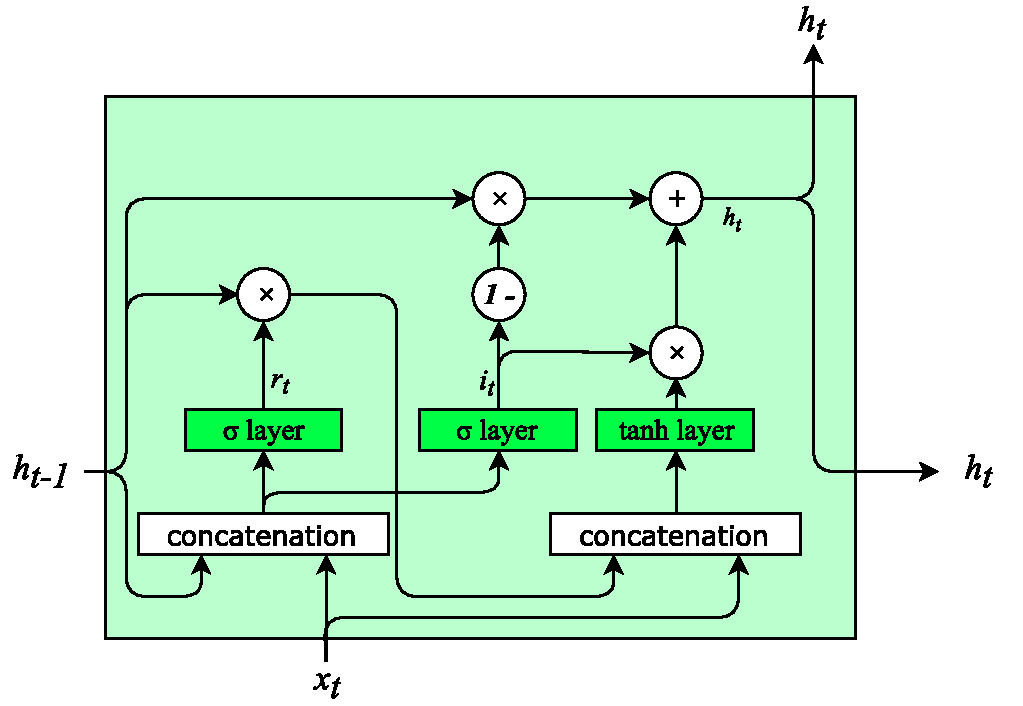
\includegraphics[max width=\linewidth,max height=8cm,keepaspectratio]{figures/GRU}
    \caption{The Gated Recurrent Unit cell porposed in~\cite{cho2014learning}}\label{fig:GRU}
\end{figure}

The advantage of this type of element with respect to LSTM is that less parameters are used.

Figure~\ref{fig:GRU} shows the internal composition of the cell. The analysis of how the internal layers are connected can be done by taking as reference the simple RNN with only the  \( tanh \) layer. GRU firstly adds the reset gate  \( r_{t} \) that modulates how much of the previous state  \( h_{t-1} \) is passed to the basic  \( tanh \) layer. The other gate, the update one  \( i_{t} \) decides the weighting between the basic  \( tanh \) output and the previous state  \( h_{t-1} \) : if the values are close to  \( 1 \) , the cell works similarly as a simple RNN that suffers from long-dependencies irrelevance (fading gradients), but as the values of this gate decrease the behavior of the cell tends to keep its state unchanged.

It is important to notice that this cell has only one state vector: no distinction between visible  \( c_{t} \) and hidden  \( h_{t} \) , the architecture is simpler.

Being more recent, less studies have used them, but from the performance point of view, they seem to be of the same order of LSTM (like~\cite{jozefowicz2015empirical} and~\cite{chung2014empirical}).

\subsection{Word embeddings}
\label{soaWordEmbeddings}

Now that the bases of recurrent networks have been described, let us focus on a very important point: inputs. The choice of the inputs to the neural network is very important and can affect a lot its performances.

It might seem that we already have the inputs to the Neural Network: sentences. Sentences are made up of words and we would like to use those words as inputs to the classifier network.

But since all neural networks only work with numbers, there must be a layer at the beginning that, given the input words, transforms them in numerical form.

The most simple and naive approach is to consider the $``$one-hot$"$  vector of the words. This representation is an array with length corresponding to the length of the input dictionary and contains values that are all zeros except for the one whose index corresponds to the index of the word in the vocabulary. In other words, a dictionary is built and the representation of the i-th word in the dictionary is an array with a single non-zero value on the i-th value. This is straightforward to implement, but has some problems because highly depends on the input dictionary: the length of one-hot vectors is the same as the length of the dictionary. Any network following this representations will have a big problem: different words, with similar meanings, will be completely different so any parameter that can be learned on one words will not be applicable to a similar word. This approach cannot work with words that are not contained in the training set.

Other solutions may employ techniques like stemming or lemmatization, that try to reduce the vocabulary by stripping out word suffixes and reconduce words to their roots. Stemming, applies brutally some rules to remove the suffixes, while lemmatization extracts the lemma with more powerful and studied rules. However those techniques remove information that could in some way be useful, and make human language very rich.

A better approach is to use a representation of words that considers semantics and syntactic information. The hypothesis behind this method is the Distributional Semantics~\cite{sahlgren2008distributional}:\ words that appear in the same context (the context is there defined as the surrounding words) are considered similar, because somehow they can be exchanged the one for the other since they appear in similar contexts. With this hypothesis, each word is mapped to a dense real vector with a fixed dimension,  where the values are optimized to represent the semantical distribution of the corresponding words. Their dimension is a lot smaller than the size of the input dictionary. The word embeddings are usually pre-trained on large corpora of unlabeled data (for example Wikipedia\footnote{\url{https://dumps.wikimedia.org/}} or CommonCrawl\footnote{\url{http://statmt.org/ngrams/}}).

With these vectors it is possible to perform different things:

\begin{itemize}
	\item Find neighbors and compute the similarity of words;

	\item Visualization on 2D plane~\cite{maaten2008visualizing};

	\item Mathematical operations with words that represent analogies of relationships among words: this can be measured with the so called \textit{analogy test~\cite{mikolov2013linguistic}}.
\end{itemize}

Using word embeddings as inputs to the neural network has the advantages~\cite{bengio2003neural}:

\begin{itemize}
	\item Reduced size of input arrays, no $``$curse of dimensionality$"$ ;

	\item Semantic and syntactic similarities of words are considered.
\end{itemize}

The embeddings can be part of the model (in this case the weights of the embedding layer are trainable) or can be pre-computed on external bigger corpus. The first option is preferred when the size of the used corpus is big enough and it is thought to be comprehensive enough in terms of word coverage (no unexpected new words in prediction time). Instead when the corpus of the considered problem is not big enough to model the word distribution in terms of syntax and semantics, it is better to use pre-trained word embeddings.

Pre-trained word embeddings can also be fine-tuned. Fine-tuning has as main advantage to reduce the loss on the desired task, but can also have some disadvantages: if two words are $``$near$"$  in the pre-trained embedding space, and only one of them is used in a neural network and fine-tuning is applied, the position in the embedding space can change and move far from the other word, not trained in the model. If the other word occurs in model testing (inference), the network will have some problems because the two words are not anymore similar.

Machine Learning approaches that use word embeddings to translate from words to representations that capture their meanings are said to be \textit{semantic}.

\subsubsection{The algorithms}
There are different algorithms for producing word vectors, that fall into two families: count based and direct prediction. For the count based ones, the idea at the basis is to build a co-occurrence square matrix with the dimension of the vocabulary. Then, chosen a window size (usually between 2 and 5) the chosen corpus is processed by sliding this window over the words and the counts are collected. Once this matrix is filled up, some strategies for dimensionality reduction are applied. Usually \textit{Singular Value Decomposition~\cite{golub1970singular}} is used, a particular matrix factorization technique based on the usage of eigenvalues and eigenvectors. Without entering in the mathematical details, we can view that as a trick to translate the co-occurrence matrix into the word vectors, keeping the idea that words with similar occurrence count correspond to similar word vectors, and therefore similar meaning due to the distributional hypothesis.

The second family instead, direct prediction, puts the calculation of those vectors under the machine learning technique: the values for each word are used as tunable parameters that need to be optimized through a learning procedure. The problem is defined as follows: considering the same sliding window of words as the count based, for each center word the contextual words inside the window are considered, and the objective is to predict the one from the other. In detail, two different models exist: the CBOW (Continuous Bag of Words) predicts the center word from the outside context words and the skip-gram that instead predicts the context words from the central one. These two possibilities exist for the \textit{Word2Vec }algorithm described in~\cite{mikolov2013efficient}, and what emerges is that the first one is better on smaller datasets because it uses all the surrounding words to perform a single observation smoothing the distributional information, while the second one is able to produce more detailed predictions over large dictionaries because treats each word in the context is treated as a new observation.

Other algorithms do a hybrid approach, mixing count-based with direct predictions. This is the case of GloVe~\cite{pennington2014glove}. All these solutions work on the word level only. Instead some works have been done also to enrich the representations with subword features. In~\cite{bojanowski2016enriching}, following the idea that similar groups of letter convey similar meanings, each word is mapped to a set of \textit{n-grams} and the skip-gram model is changed to consider each word vector as the sum of its n-grams. Figure~\ref{fig:fastText} shows an example of extraction of n-grams (with  \( n=3 \) ), where the first and the last ones contain some special characters to indicate the beginning and end of words. The learning of the embeddings therefore is not done on the words but on the groups of letters. In this way it is possible to compute word vectors also on unknown words since they are composed of known n-grams.

\begin{figure}[!htbp]
    \centering
    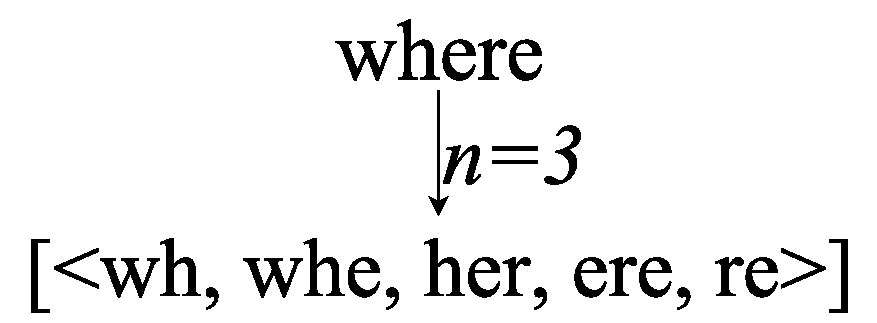
\includegraphics[max width=\linewidth,max height=8cm,keepaspectratio]{figures/fastText}
    \caption{An example of the n-grams derivation of FastText in~\cite{bojanowski2016enriching}}\label{fig:fastText}
\end{figure}

\subsubsection{The vocabulary issues}
\label{soaVocabulary}

Having good algorithms for word embeddings is a good starting point. But there may be some problems when deciding how to preprocess the corpora. What we want to consider as input features? Only the words in lowercase, cleaned up from all the non alphabetical characters, or we may consider other hints from the user typing such as capital letters or punctuation?

The choice is usually to clean deeply the inputs in order to reduce the vocabulary. For capitalization it means to lowercase everything. But the casing feature may be important in some way to help recognizing entities (think about a place name with capital letter, or an acronym uppercase). On the other side, beginning of sentences have capital letters that should be lowercased because that is not a wanted feature, it is only required by writing rules. For this reason some invented a truecasing model~\cite{lita2003truecasing} that aims at reconstructing the correct word casing.

The other critical point is punctuation: a decision is needed about whether to keep those signs as additional dictionary entries or simply drop them. A very critical one is the apostrophe: the words around it are usually modified, so not only they have to be considered separately, but also some reconstruction could be required (example: $``$\textit{we're}$"$  as a single word  \(  \left[ "we're" \right]  \)  or separating by the apostrophe  \(  \left[ "we", "'re" \right]  \)  or reconstructing the original words  \(  \left[ "we", "are" \right]  \)  in order to have the same entry for the verb  \( "are" \)  in the dictionary (or applying a stemmer with similar results).

An approach based only on alphabetical lowercased words may be good for scenarios where the users do not have the time to write complex punctuations. But when additional features are provided (such as punctuation and word casing in text, and accents and tone in voice), it would be a pity to throw away things that may be useful for doing a better classification.

\subsection{Intent classification}
\label{soaIntent}

Let us talk here about approaches for the first task of NLU, intent classification, that takes as input the sentence and provides as output a label that corresponds to the intent type of the sentence. It is a multi-class classification. It takes in input a sequence of words and produces a single label, that is a trait value of the input sentence.

\subsubsection{Keyword-based}
The first approach that can be considered is keyword-based. In this approach, for each intent type we determine a set of keywords that, if present in the current input, gives a score to the selected intent type. For example a naive classifier can be built to generate keyword groups from training sentences and classify accordingly to their presence by doing a $``$majority vote$"$  on the words of the current sentence.\footnote{\url{https://chatbotslife.com/text-classification-using-algorithms-e4d50dcba45}} This approach dynamically determines the keywords for each class, but it is not good enough because it looks only at some words in the current input sentence.

A better idea would be to compute a sentence-level representation that summarizes all the words and the meaning of the sentence, and from this vector it does a classification on the output labels (intent types). For this sentence vector a lot of different approaches can be applied that are explored in the following paragraphs.

\subsubsection{Average of word vectors}
First of all, given the word vectors for each word contained in the sentence, an average can be done. As shown in Figure~\ref{fig:intentAverage}, after the average is computed over the fixed-length embedding values for the input words, a simple feed-forward layer can be used to map to the intent space, producing logits that estimate the probability to belong to a certain class (intent type).

This strategy however is not good because it does not consider the order and the relationships between the words. The order matters a lot in natural language.

\begin{figure}[!htbp]
    \centering
    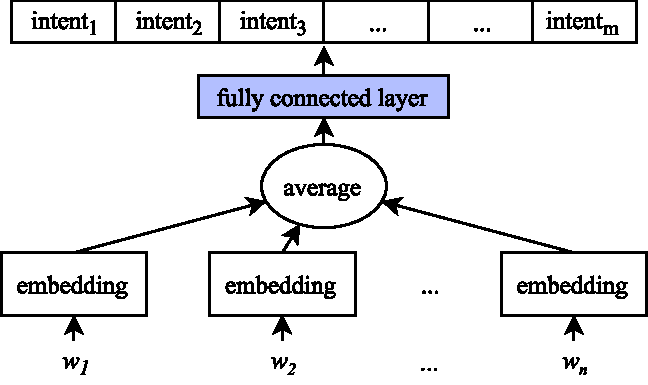
\includegraphics[max width=\linewidth,max height=8cm,keepaspectratio]{figures/intentAverage}
    \caption{Intent classification by average of word vectors}\label{fig:intentAverage}
\end{figure}

Another problem of this approach is that actually every word counts the same, so if stopwords are not eliminated they can bias the output basing on irrelevant inputs.

\subsubsection{RNN approach}
To consider the order, a RNN can be used to summarize the sentence and produce a sentence representation that can be used in another layer to classify on the intent types. The output of the RNN is taken only at the end of the sequence. This approach is able to capture some more information about the sequence that considers the relative order of words. Considering both a forward and a backward RNN, the output of the summarized output is not biased towards the end of the sentence as would happen for a forward-only RNN. Figure~\ref{fig:intentBidirectionalRNN} shows how the bidirectional encoding of the sentence substitutes the average operation with respect to the previous approach. The output projection layer finally performs the mapping to the intents spaces.

\begin{figure}[!htbp]
    \centering
    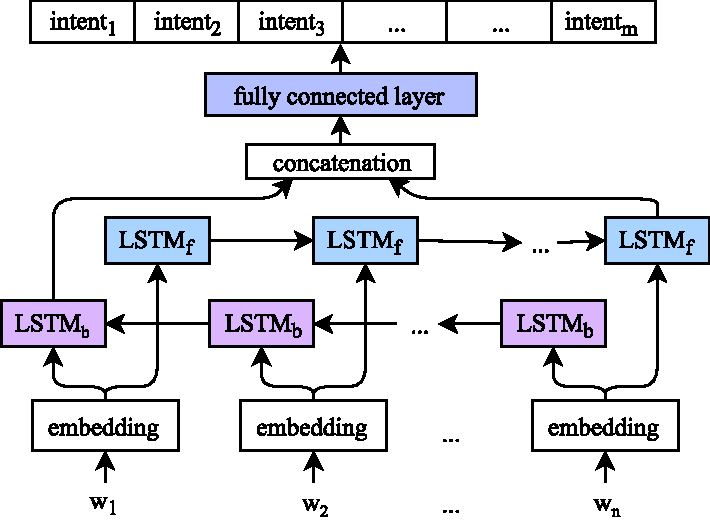
\includegraphics[max width=\linewidth,max height=8cm,keepaspectratio]{figures/intentBidirectionalRNN}
    \caption{Intent classification by applying a bidirectional RNN}\label{fig:intentBidirectionalRNN}
\end{figure}

What makes this technique to work well is that the LSTM is very good at capturing sequence-level information, considering with different importance the input words. The problem of stopwords is defeated and the Recurrent Network learns to discard the irrelevant words.

\subsubsection{RNN with attention}
To emphasize the fact that some words count more than others in the classification problem, several techniques can be used. First of all, \textit{stopwords} can be identified and removed. But more dynamic approaches can automatically learn a distribution over time of words that tells how much relevant is this word for the task. This is the attention mechanism, that is quite commonly adopted in automated translations~\cite{bahdanau2014neural} and on sentiment analysis~\cite{lin2017structured}.

This kind of additional component, as will be seen also for the slot filling task in \ref{sequenceAttention}, provides a way both to learn those scoring values and to use them for a weighted average on the outputs of the RNN layer. In the case of intent classification the attention wraps the bidirectional RNN.

\subsection{Sequence-to-sequence models for slot tagging}
\label{soaSeq2Seq}

The task of slot tagging instead consists of generating an output sequence in which each element corresponds to a tag for the corresponding input word. The tag can be the entity type or the IOB. IOB can be useful when there is the need to deal with multi-word slots, as in the example of Figure~\ref{fig:iob}.

A lot of the architectures listed below have been created for the task of Neural Machine Translation. This task takes as input the sequence of words in the source language and outputs a sequence of words in another language. This is somehow similar to the task of sequence labeling, because it maps an input sequence to an output sequence, but has some differences that make it a lot different and require a different approach. The differences will be explained in details during the analysis.

A common characteristic of them is the presence of two key elements: an encoder and a decoder. The encoder is responsible of collecting all the useful features on the input sequence. The decoder instead must generate the output sequence. The differences between the different models are on the way that the encoder provides input to the decoding stage. The general composition of such encoder-decoder approaches is shown in Figure~\ref{fig:encoderDecoder}

\begin{figure}[!htbp]
    \centering
    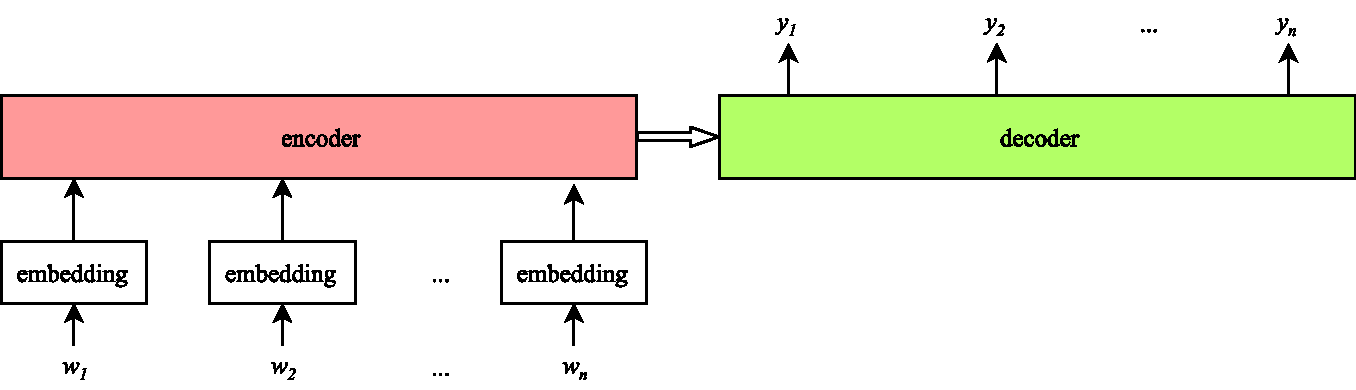
\includegraphics[max width=\linewidth,max height=8cm,keepaspectratio]{figures/encoderDecoder}
    \caption{The connections between Encoder and Decoder components for sequence translation}\label{fig:encoderDecoder}
\end{figure}

A very critical point when generating the output sequence is the correlation between the IOB labels. For example a $``$\textit{I-ent}$"$  is always preceded by a $``$\textit{B-ent}$"$  or another $``$\textit{I-ent}$"$ . Also there can be some patterns that highlight that after a certain entity it is more probable to find another one. This is called output dependency, that occurs at the decoding stage, just before the production of the outputs. 

Modeling the output dependencies can be done in different ways:

\begin{itemize}
	\item Local choice: using this approach, each decoding step produces an output that is then projected to the labels. The decision about which labels to assign is done locally, performing a simple softmax operation followed by a sampling;

	\item Feed the previous output together with the current input to decoding timesteps: (similarly to a Jordan Network~\cite{jordan1997serial}) in this approach, the output is fed back as input to the next timestep for the decoder network, and the network in training learns the output dependencies;

	\item Linear-chain CRF: an alternative to RNN for modeling the output dependencies is using a linear-chain CRF. This can substitute the decoder network, and use the encoder to produce its input features. CRF finds the paths with higher energy in a very similar way to RNN. In other words, it finds the output sequence that is mostly probable;

	\item Beam search: not only a single candidate is kept for subsequent decoding timesteps, but a set with fixed size, in order to be able to perform decoding without always following the local optimum.
\end{itemize}

In the following paragraphs we give a description of some sequence-to-sequence approaches, from the most simple ones towards the most suitable for the slot labelling task.

\subsubsection{Simple Encoder-Decoder}
The most simple approach, illustrated in figure~\ref{fig:encoderDecoderRNN} is the one where the encoder collects all the word vectors and using a RNN computes a final representation of the sentence (as in the intent classification task). This representation is passed to the decoder RNN that for each timestep produces an output word.

\begin{figure}[!htbp]
    \centering
    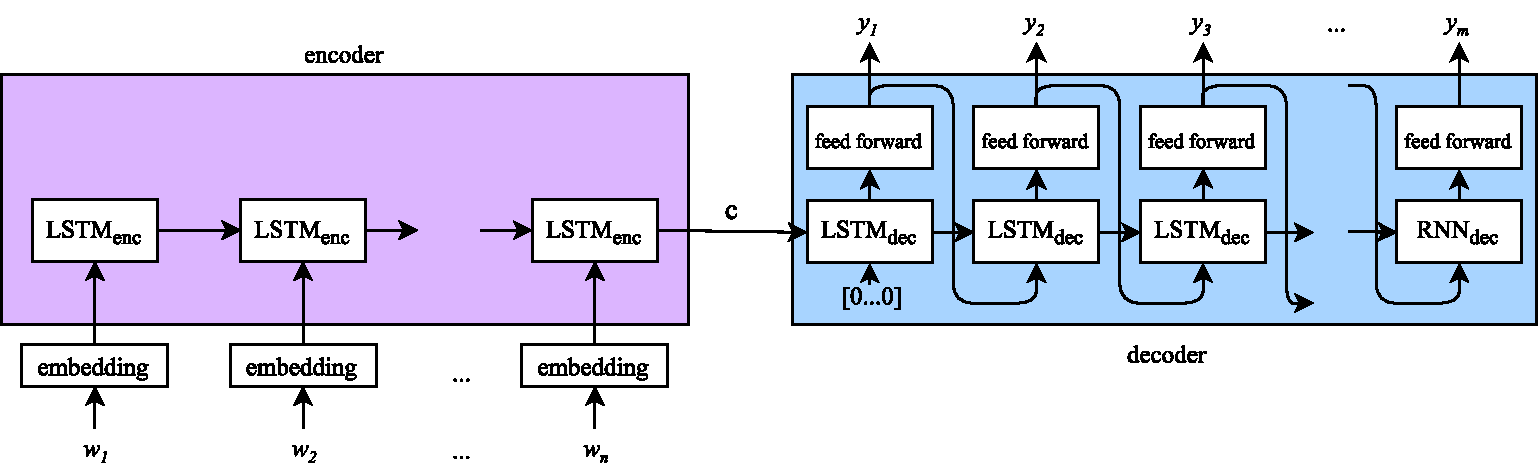
\includegraphics[max width=\linewidth,max height=8cm,keepaspectratio]{figures/encoderDecoderRNN}
    \caption{The usage of RNN for a simple Encoder-Decoder approach}\label{fig:encoderDecoderRNN}
\end{figure}

This model has some problems. First of all, the decoding part depends only on the sentence vector c, that must be able to keep all the information on the input sequence, whose length can vary, in a fixed size. Then, the decoding steps may easily lose the relevant information from this vector, since the decoding can take a lot of decoding timesteps. But a much greater problem comes from the lack of constraint on the output sequence length: in translation between different languages, this can be a good feature, but in our task of sequence labeling we want an output sequence with fixed length. The last observation we can make is that there is no alignment model between the input and output sequences. The outputs depend on all the inputs, without having different encoded information for the decoding of the output sequence.

\subsubsection{Encoder-decoder keeping sentence vector}
This model comes from~\cite{cho2014learning}, a study on the task of neural machine translation. It is an enhanced version of the previously considered model because the sentence vector coming from the encoding stage is passed to all the decoding stages (see Figure~\ref{fig:encoderDecoderKeepC}).

\begin{figure}[!htbp]
    \centering
    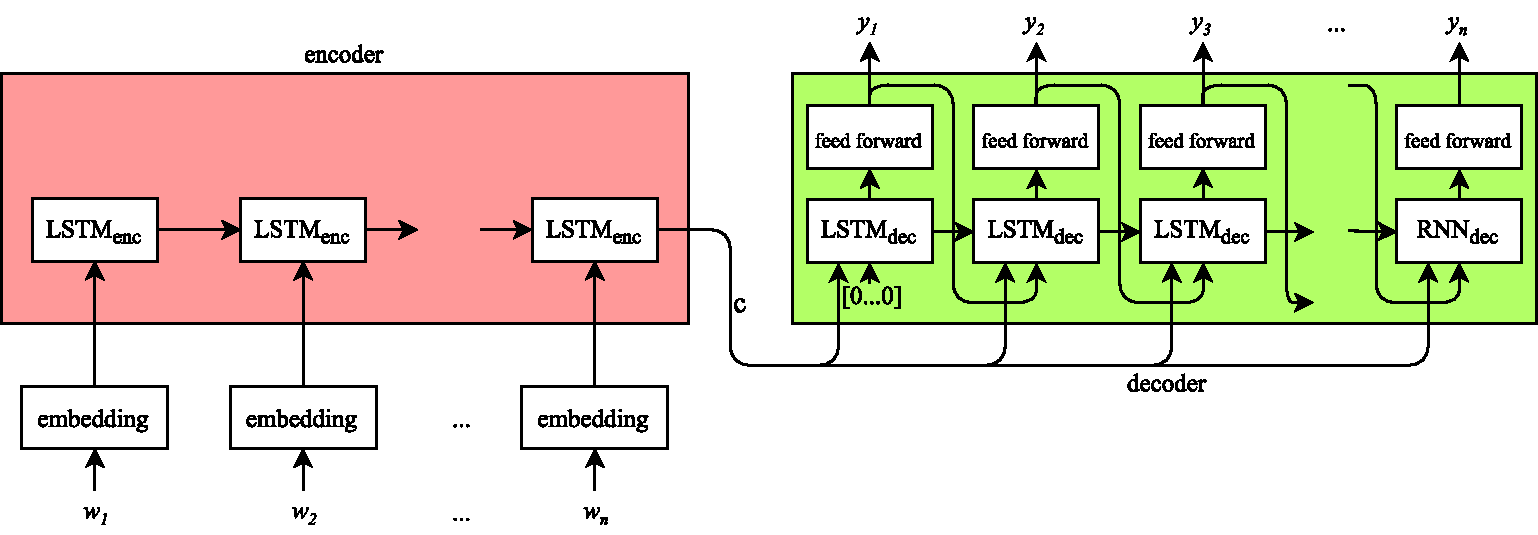
\includegraphics[max width=\linewidth,max height=8cm,keepaspectratio]{figures/encoderDecoderKeepC}
    \caption{Passing the sentence vector to all the decoding steps}\label{fig:encoderDecoderKeepC}
\end{figure}

This approach helps the decoding stages that, receiving the sentence vector directly, can perform better in their task. However, some problems are not solved: the output sequence length has no constraints and there is no alignment model.

\subsubsection{Encoder-decoder with aligned inputs}
This model was proposed~\cite{liu2016attention} for the sequence labeling problem (that can be applied to slot filling, POS tagging). In this model the encoder sends some information to the decoder for each input word instead of sending a single vector at the end (see figure~\ref{fig:encoderDecoderAligned}).

\begin{figure}[!htbp]
    \centering
    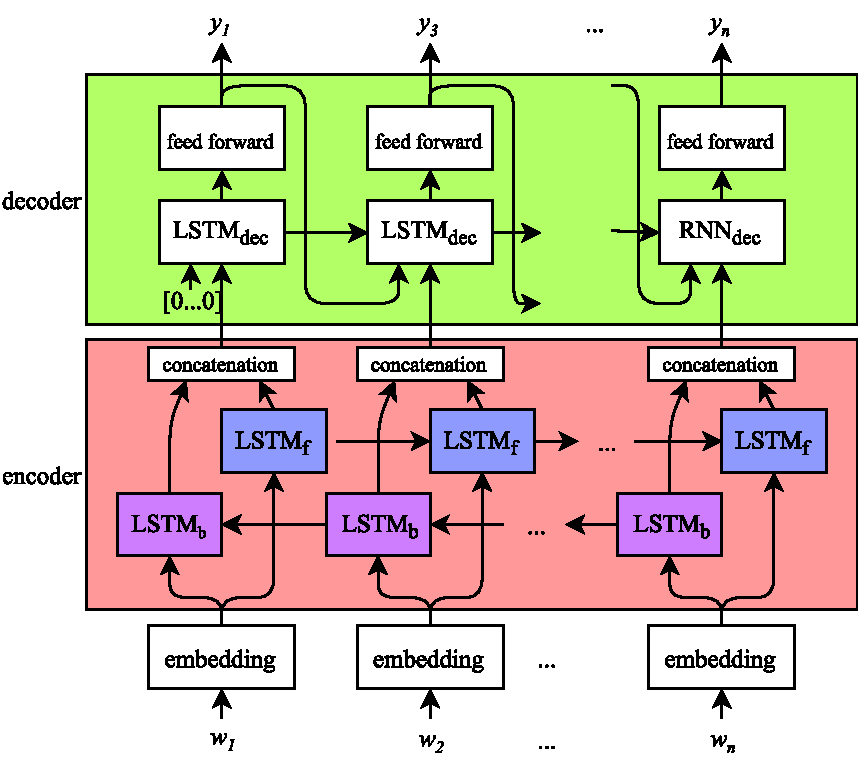
\includegraphics[max width=\linewidth,max height=8cm,keepaspectratio]{figures/encoderDecoderAligned}
    \caption{The Encoder-decoder with aligned inputs: each decoding step is influenced by the contextual representation of the aligned word}\label{fig:encoderDecoderAligned}
\end{figure}

This model fixes the output sequence length to the length of the input sequence. The alignment model is fixed: the decisions in decoding are done looking at current input word in the current left plus right context.

\subsubsection{Encoder-decoder with attention}
\label{sequenceAttention}

The idea of attention empowers recent studies on translation. The purpose is to decide which outputs of the encoder are more relevant for the current decoding step dynamically. On the previous model, always the aligned encoded input is used, but for language translation this can be a limitation.

Using the attention~\cite{bahdanau2014neural}, that provides a dynamic alignment model, it is possible to:

\begin{itemize}
	\item Determine which are the encoded inputs that are more relevant;

	\item Use them to provide a better translation.
\end{itemize}

\begin{figure}[!htbp]
    \centering
    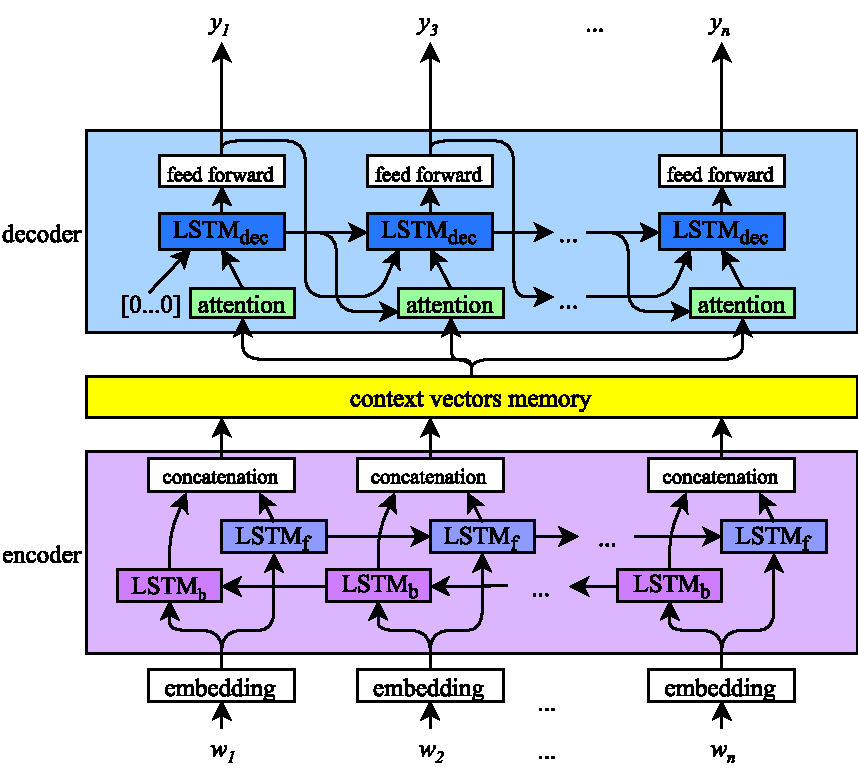
\includegraphics[max width=\linewidth,max height=8cm,keepaspectratio]{figures/encoderDecoderAttention}
    \caption{The aligned Encoder-decoder with the addition of attention mechanism}\label{fig:encoderDecoderAttention}
\end{figure}

The attention, as can be seen in Figure~\ref{fig:encoderDecoderAttention}, adds two blocks: one is the context vector memory, which stores the output of the bidirectional RNN at each timestep, and the other one is the attention block that is responsible to pick up the correct mix of the encoded vectors by doing a weighted sum of them and provide that to the decoder RNN. 

By looking inside at the \textit{attention} mechanism, in Figure~\ref{fig:attention} we can see that the encoded vectors  \( e \)  are used together with the previous hidden state of the decoder cell  \( h_{i-1} \) in some matricial multiplications and finally pass through a softmax. This part is responsible to learn the weights for each timestep of the decoder that represents how much relevant are the input words for the determination of the current output word. The matrices  \( W_{1} \) , \( W_{2} \)  and  \( V \) are used together with a  \( tanh \)  layer to determine dynamically those weights. This block, put inside a complex network architecture, learns all the parameters thanks to the backpropagation algorithm being end-to-end differentiable. The output  \( c_{i} \)  is then computed doing a weighted sum between the  \( e_{j} \)  encoded vectors.

\begin{figure}[!htbp]
    \centering
    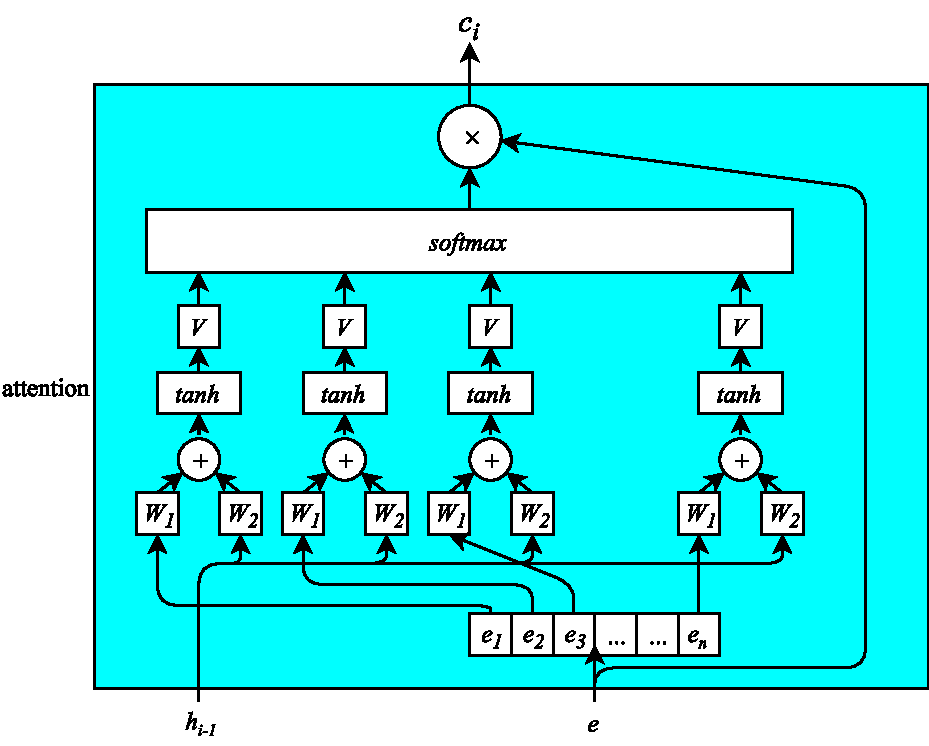
\includegraphics[max width=\linewidth,max height=8cm,keepaspectratio]{figures/attention}
    \caption{How the Attention block computes a weighted sum, learning the weights dynamically}\label{fig:attention}
\end{figure}

With this network, used for translations, it is useful to show how the attention maps the words in the two languages. Figure~\ref{fig:attentionVisualization} shows a matrix representation that says which input words were used to provide the corresponding output words.

\begin{figure}[!htbp]
    \centering
    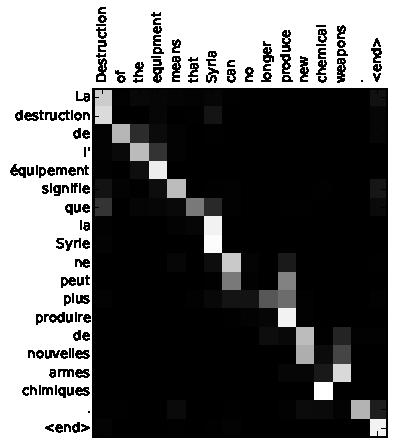
\includegraphics[max width=\linewidth,max height=8cm,keepaspectratio]{figures/attentionVisualization}
    \caption{A visualization of the attention scores in translation~\cite{bahdanau2014neural}}\label{fig:attentionVisualization}
\end{figure}

The attention model is quite advanced, and since a lot of other parameters are there in the network, a lot more of training samples must be used.

For the task of sequence tagging it seems to be too much. The output labels depend only on the current word context that is already given by the bidirectional encoder RNN, so the expected values for the attention distribution is that it will keep the inputs and outputs aligned. It can be kept together with the aligned model just to provide more features.

\subsection{Joint tasks}
The two tasks can be combined together in one single network in different ways and with a wide variety of additional things that can be added (for example attention mechanism, output dependencies). The approaches found in literature try to use a common encoding stage and then differentiate on the decoding, one for each task. The network has to fork at some point because the shape of the outputs is different: one single label for the intent and many slot labels, considering a single input sentence.

In~\cite{liu2016attention} there are two different proposed architectures: one is based on the encoder-decoder adding the intent output, while the other collapses all in one single compact structure.

The first one, as can be seen in Figure~\ref{fig:jointSLUAligned}, is a combination of the bidirectional RNN for intent classification and the encoder-decoder with attention for the slot filling. The two networks, having the encoder in common, are merged together, and fork for the following layers towards two different outputs.

\begin{figure}[!htbp]
    \centering
    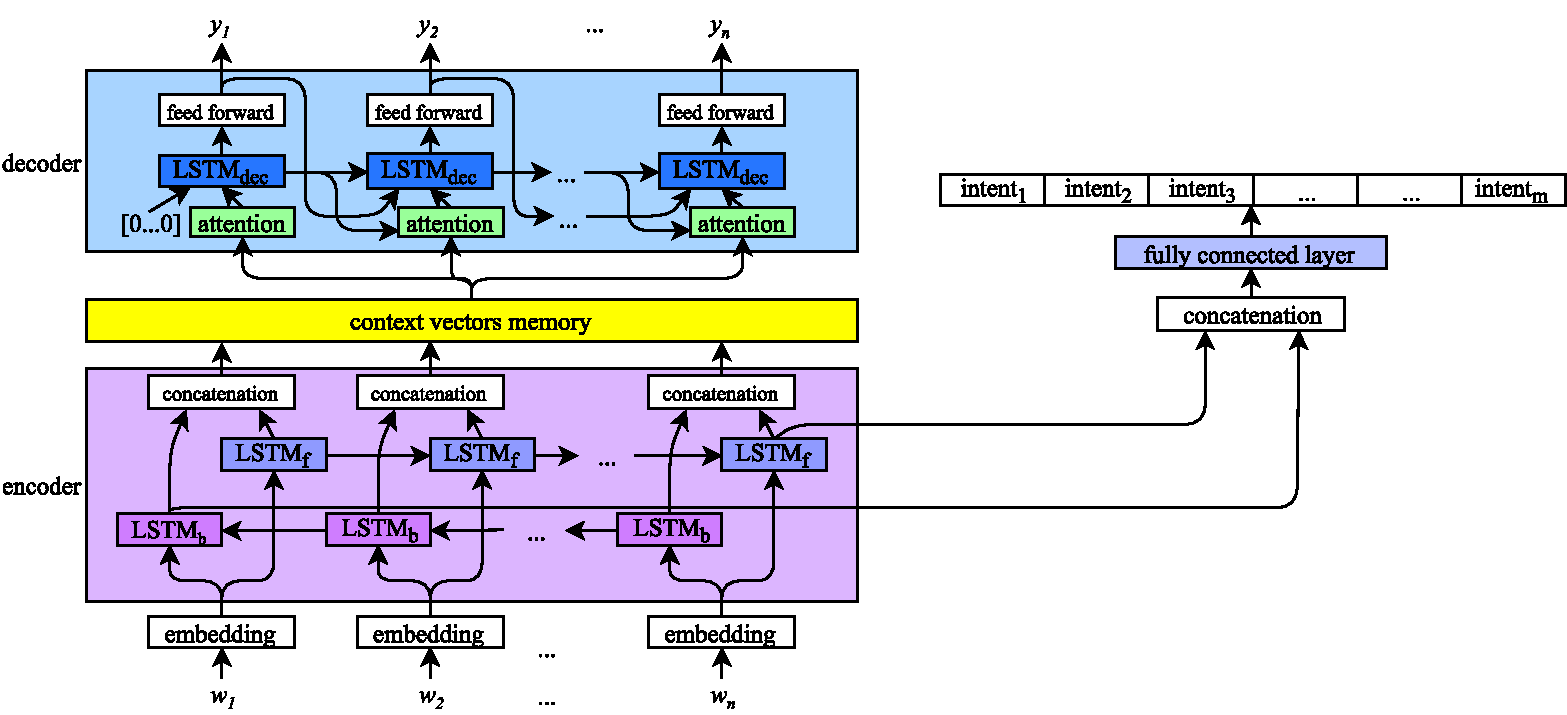
\includegraphics[max width=\linewidth,max height=8cm,keepaspectratio]{figures/jointSLUAligned}
    \caption{The Joint Encoder-decoder model with Aligned Inputs in~\cite{liu2016attention}}\label{fig:jointSLUAligned}
\end{figure} 

The two branches consider different outputs of the encoder. The intent classifier is added as a branch that takes the last state of the encoder and then projects to the intent space with a single layer feedforward. Instead the slot filling decoder takes all the word-level outputs because it needs an aligned model.

The other network proposed in the paper is a bit different. Instead of having a separate RNN for encoder and decoder, it has a single bidirectional RNN, that in the forward direction also has the modeling of slot label dependencies. As can be seen in Figure~\ref{fig:jointSLUrnn}, the intent classification is done on top of the bidirectional RNN output, doing a mean pooling on the states at each timestep or, if the attention is enabled, by using a weighted average.

\begin{figure}[!htbp]
    \centering
    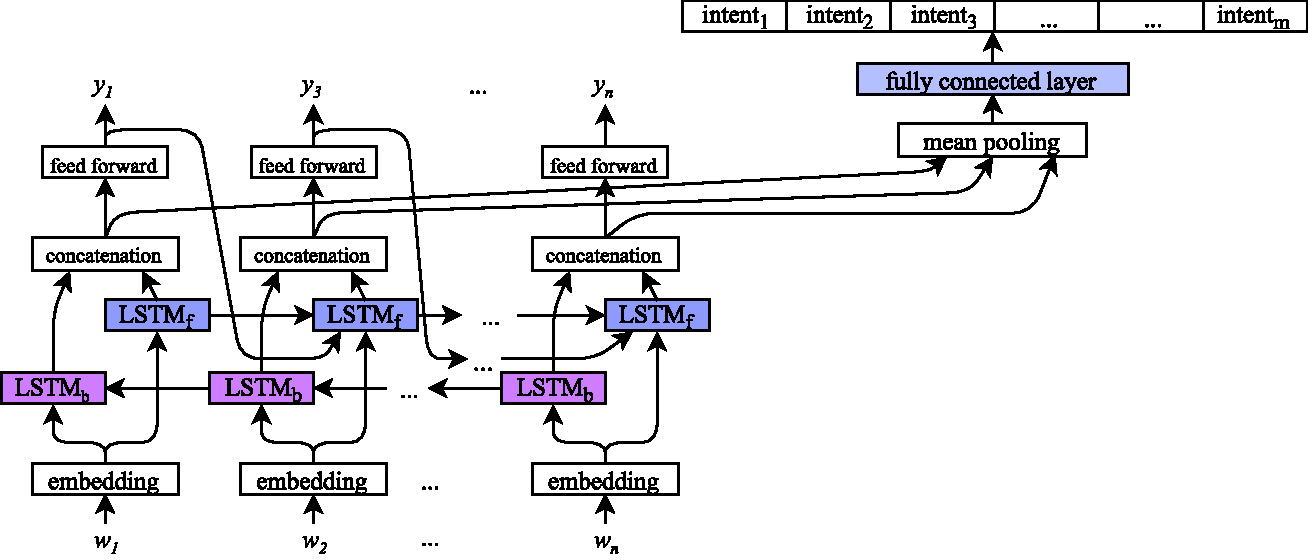
\includegraphics[max width=\linewidth,max height=8cm,keepaspectratio]{figures/jointSLUrnn}
    \caption{The joint attention-based RNN Model in~\cite{liu2016attention}}\label{fig:jointSLUrnn}
\end{figure}

\subsection{The interaction context}
\label{soaInteractionContext}

All the previously described networks only care about the current sentence, but human natural language understanding does not limit itself on this strict form. What happens when we meet some people that are already talking about something? It may take some time to understand the topic of the discussion, we need to collect some information as the interaction goes on to get the point of the discussion. This happens because most of the sentences are not standalone, but they belong to a context that goes beyond the single sentence.

The \textit{context} of a conversation can be defined as a set of important things to know in order to both understand others and say more relevant things. The context can capture features belonging to different areas:

\begin{itemize}
	\item domain: knowledge of the topic of the discussion. A conversation where the participant have a deep knowledge of it brings an exchange of meaningful ideas and opinions;

	\item interaction: going beyond the fixed form of atomic question-answer pairs. Human to human conversations rely a lot on the interaction context, referring explicitly or implicitly to things that have been previously said. A multi-turn environment can allow users to do questions and later refining them to find what they were searching for, by simply adding new parameters instead of rebuilding a complete independent interrogation, or doing follow-up questions on the previous results;

	\item interlocutor: knowing better the user that we are interacting can be advantageous to find better and targeted responses to his question, both in the form and in the content.
\end{itemize}

In this work we focus more on the interaction context because it is the one that is mostly related to language. The domain knowledge is instead given by design in goal-oriented bots, because they are built to serve some specific needs and do restrict the topics of conversation. Instead for the interlocutor/user context, it is the field where the personalization techniques are analyzed, as will be seen in Section \ref{soaPersonalization} for the background and in Section \ref{approachPersonalization} for more dialogue-related personalization techniques.

The interaction context feature can be seen as some kind of memory that actors in a conversation need to keep about previous sentences. The context is necessary to understand the dialogue at different levels:

\begin{itemize}
	\item Understand the role of some words in a sentence given some information contained in other sentences. This practically means to identify entities by knowing that after a certain type of question it is easier to find them (e.g. replying to $``$\textit{Where?}$"$  questions suggest that the next sentence contains a place entity, even if the sentence does not contain indicators like $``$\textit{near/in/at}$"$ ). We may call this setting \textit{multi-turn slot filling}.

	\item Understand the meaning of the current sentence. This is the case of sentence classification, like extracting the intent, when the current sentence does not give hints about it, but a knowledge of the previous sentences can lead to the correct understanding (e.g. replies like $``$\textit{ok. Let's do it}$"$  that standalone are impossible to be processed). We call this the \textit{multi-turn intent classification}.

	\item Ability to link the all the entities that are mentioned in a discourse, being able to resolve the things that are behind words like $``$\textit{this/him}$"$ . This is the \textit{coreference resolution}.

	\item Based\ on previous levels, link the meanings of things across the different turns, and be able to answer to some test questions that require reasoning. This is the so called  \textit{dialogue tracking}.
\end{itemize}

All those levels of understanding provide active fields of research in the NLP community and they fall under different names. The first one is \textit{multi-turn} appearing in~\cite{chen2016end},~\cite{chen2017dynamic},~\cite{xu2014contextual},~\cite{bhargava2013easy} and~\cite{shi2015contextual}. This term is specific to virtual assistants and it covers the first two levels of understanding: the goal is to identify the intent and entities in a dialogue where the user is not using a single sentence to ask for information. One common case is when, after the initial question of the user, the agent asks back for some clarifications or missing parameters to refine the search. In this case the assistant should put together the information contained both in the current sentence and in the previous ones, to perform a complete query. Other common cases are user follow-up questions. Receiving some results from the agent, the user could ask for more details or to change some parameters. In this case, the user refers to the previous query and it is only changing some constraints (like the intent or some slots).

The other used term is \textit{dialogue state tracking}: mostly known because of the Dialogue State Tracking Challenge~\cite{williams2013dialog}, it refers to the ultimate level of understanding a dialogue: represent the dialogue state and updating it as the conversation keeps going on.

Different solutions exist and depend on where we want the neural network to come in contact with the application logic (what to establish as manual rules and what is inferred by the neural network approach). Literature shows case studies where there is a strict separation between the understanding module and the management of the dialog state~\cite{liu2016attention}~\cite{chen2016end}, but also cases where everything is put together in an end-to-end fashion in a way more independent from domain rules~\cite{serban2016building}~\cite{eric2017key}.

In the first type of systems, the NLU module contains the recurrent neural network stuff and produces as output intent and slots. Once they are extracted from the dialogue, another module $``$dialogue state tracker$"$  keeps track of the conversation and applying some handwritten rules decides the flow of the conversation and provides responses back to the user.

Instead in the end-to-end architectures, all the components are trained by dialog examples. The positive point is that there is no need to handwritten rules for the dialogue state tracker. The rules are inferred by the dialog corpus and the system learns what is the most appropriate answer to provide. Some parts are still not part of the trainable model: the module accessing the data exposes some operations via some API. The trainable model learns when to issue API calls. However, the end-to-end approaches need a very big amount of dialogues to induce the general rules giving an advantage to rule-based dialogue tracking systems where the resources are limited.

The following paragraphs explore the three levels of interaction context that have been outlined previously.

\subsubsection{Multi-turn Understanding}
As mentioned before, the goal of multi-turn SLU is simply to extract the intent and the entities when the user is not providing a single sentence with all the required parameters. In a second moment, it could be after the agent asks back for some parameters, other sentences complete the initial one with more entities that are used to refine the search. It can be seen as an iterative filling of a fixed-structure form. For this reason, a naive approach could be simply to classify the intent on the first sentence and then collecting the parameters in a key-value fashion (the key is the name of the slot, that is asked by the agent, and the value is the answer taken $``$as is$"$ , as can be seen in Figure~\ref{fig:multiTurnFilling}).

\begin{figure}[!htbp]
    \centering
    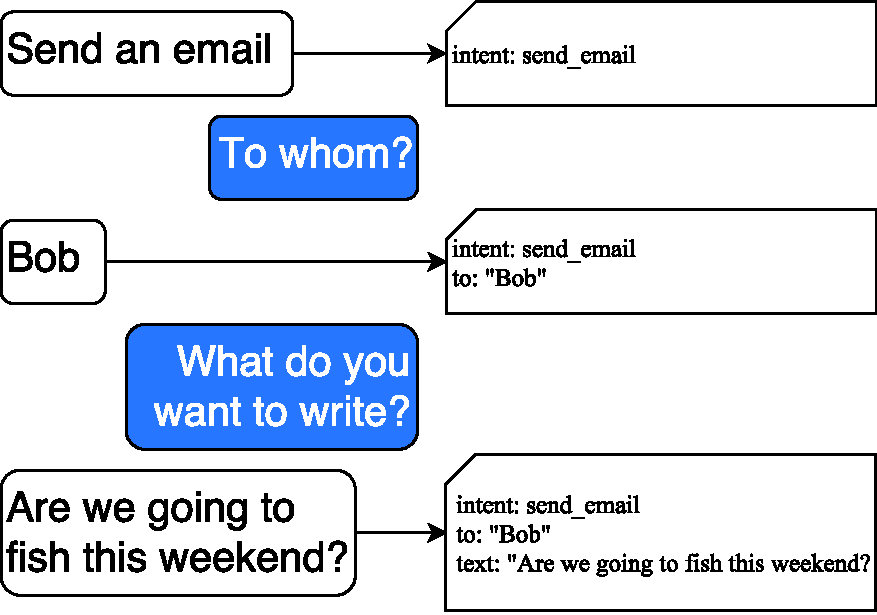
\includegraphics[max width=\linewidth,max height=8cm,keepaspectratio]{figures/multiTurnFilling}
    \caption{A simple dialogue where a simple key-value approach can provide multi-turn abilities}\label{fig:multiTurnFilling}
\end{figure}

This approach is quite simple but has some problems: this is not natural language. Natural language dialogue has not this fixed structure, and the system must be able to receive a sentence that contains more than a single entity. Another issue is that the user may change his mind in the middle of the interaction and start a new intent. For those reasons the SLU task should be expanded to the multi-turn environment by a more complete approach. We will there analyze some proposed solutions to this problem.

Some first works in the direction of contextualized understanding have been done in~\cite{xu2014contextual} for classification of the domain (that can be seen as a coarse-grained intent). In that work, the previous output of the system is added to the inputs by enlarging the input word vectors. The authors choose as approach for single-turn developed using a  CNN~\cite{krizhevsky2012imagenet}, so the multi-turn adding the recurrent connections results in a RNN/CNN hybrid network.

Another approach that has been studied for the multi-turn problem is~\cite{chen2016end}. The idea to additionally incorporate contextual knowledge is applied with a sentence encoder that considers also previous sentences. The current sentence is processed by a RNN like in~\cite{liu2016attention}, and the addition is the contextual sentence encoder that can be seen in Figure~\ref{fig:contextualSLUchen}.

\begin{figure}[!htbp]
    \centering
    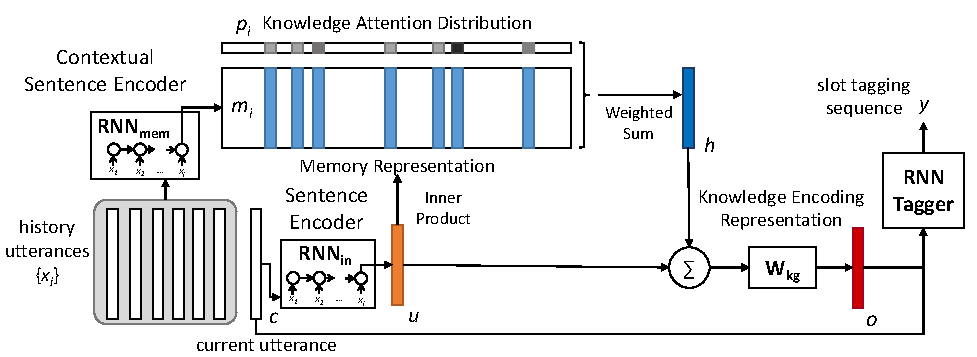
\includegraphics[max width=\linewidth,max height=8cm,keepaspectratio]{figures/contextualSLUchen}
    \caption{The contextual approach based on memory of previous turns in~\cite{chen2016end}}\label{fig:contextualSLUchen}
\end{figure}

This encoder provides a context memory representation, where each previous turn is represented. To choose which turns are more relevant for the current sentence, an attention mechanism is used in the encoded representation space. Weights for attention are computed by an inner product between the current sentence and the memory representations, which represent a measure of similarity of the considered pairs. The hypothesis behind this scoring is that sentences that have similar encoded representation should be considered more than the ones that are different. The final output of the encoding procedure is computed as the sum of the current sentence and the weighted sum of memory representations. During the decoding stage, similar to the one in~\cite{cho2014learning}, the encoded representation is used to generate slot labels.

The results of this approach have been evaluated on a proprietary dataset and therefore the results cannot be compared with other studies on the field. Furthermore in the paper the intent network is not described at all. However, this study is interesting in the perspective of how the previous sentences are considered together with the current one for the slot-tagging task.

A problem of this architecture is that the agent sentences are not considered. But the agent sentences could contain some keywords that may help to identify the slot in the decoding stage. For example if a trip requires a source and a destination, the agent asked for the source and the user answered with that, it is very relevant for the task of slot filling to know that the agent asked for source and not for the destination.

Another work has been done in~\cite{chen2017dynamic} on the value of time and roles in conversation. About the time, the idea is that most recent sentences count more and an attention score is given with values that fade out as the time is more remote. Instead for the roles, two similar networks are used, one for each role.

\begin{figure}[!htbp]
    \centering
    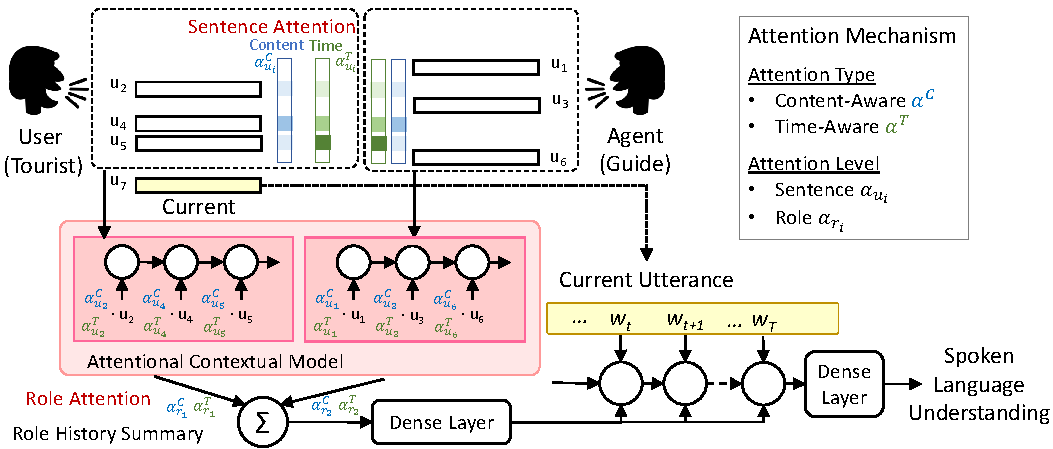
\includegraphics[max width=\linewidth,max height=8cm,keepaspectratio]{figures/timeRoleSLUchen}
    \caption{The time and role aware approach of~\cite{chen2017dynamic}}\label{fig:timeRoleSLUchen}
\end{figure}

We can see from Figure~\ref{fig:timeRoleSLUchen} that the history of sentences is encoded with different networks, one for the tourist and one for the agent. Two different mechanisms of attention are used: one is the content-aware, that is computed in the same way as in the previous mentioned paper with a dot product in the embedding space; the second one is the time-aware, that gives higher importance to recent sentences.

In this case the work has been done on the DSTC4 dataset\footnote{\url{http://www.colips.org/workshop/dstc4/}} that contains human-to-human dialogues. One of them is a tourist and the other one is a guide.

It can be seen with the progress of the DSTC over the years, that the task is switching from a multi-turn understanding to an end-to-end goal-oriented dialogue learning, as will be seen in the last paragraph of this subsection focused on DSTC6.\footnote{\url{http://workshop.colips.org/dstc6/}}

\subsubsection{Coreference resolution}
\label{soaCoreference}

The problem of coreference resolution is one of the most difficult to solve in NLP. There are currently models available to resolve explicit coreferences, using some correlation of gender and number between the entities and further references.

The problem of coreference resolution has been analyzed in TREC10,\footnote{\url{https://trec.nist.gov/pubs/trec10/t10\_proceedings.html}} as the main purpose of using the context in the sentences. In~\cite{harabagiu2001answering} a set of elements in the question, that may indicate entities mentioned in previous questions and answers, are searched. Those can be split into explicit references (such as pronouns like $``$\textit{this/that/him}$"$ , use of definite nominals like $``$\textit{the state}$"$  that suggest having a previous knowledge of reference) or implicit ones (like ellipsis of something that logically needs to be kept into consideration). The proposed system tries to find in previous turns the ones that contain the referenced entity.

A more complex approach has been analyzed by~\cite{sun2007discourse}, based on the Centering Theory~\cite{grosz1995centering} that models the local coherence of a discourse and how the transitions caused by a new sentence changes the center of the talk. In this work, two types of context are found: one depending on the user (analyzed by later TREC contextual tracks, corresponding to personalization techniques that will be analyzed in section \ref{soaPersonalization}) and the one of the discourse. The question processing should, according to the authors, perform three main tasks: \textit{i)} question type analysis and categorization, \textit{ii)} detailed processing to build and expand queries, \textit{iii)} anaphora resolution. This theory is used to build a model that selectively retain query terms from previous interactions.

Going on more recent approaches to the coreference resolution problem,~\cite{de2015modeling}\ builds a model  for predicting the lifespan of discourse entities, in other words if one of them is a singleton entity or is referenced many times. The actual scores make clear that this is yet an open field of research, where only simple sentences achieve great accuracy. A detailed description of this model is explained in an interesting online article\footnote{\url{https://medium.com/huggingface/state-of-the-art-neural-coreference-resolution-for-chatbots-3302365dcf30}} and available as an online demo.\footnote{\url{https://huggingface.co/coref/}}

\subsubsection{Simple QA to test the memory}
Going beyond the quite simple tasks of entity recognition and coreference resolution, some more difficult challenges try to address the question-answering (QA) problem relatively to the discourse. The idea is to provide some sentences that contain factual information and then an easy question is asked about this. The system has to use correctly memory abilities and combine the different facts to provide the response.

On the easiest problems proposed in~\cite{weston2015towards}, the information is contained in simple sentences that are composed by triples of subject, verb and object. Usually a model of memory~\cite{sukhbaatar2015end} is used to store the relationships between the entities expressed by the triples. From this memory the easiest questions can be directly provided, while for tasks like counting on temporal reasoning it is necessary to enable a process of machine reasoning to turn the facts into operational knowledge. Some examples can be seen in Figure~\ref{fig:toyQuestionsMemory}.

\begin{figure}[!htbp]
    \centering
    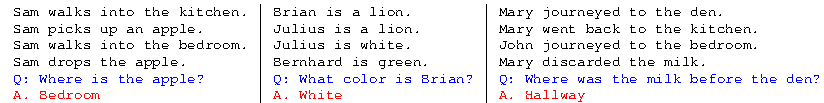
\includegraphics[max width=\linewidth,max height=8cm,keepaspectratio]{figures/toyQuestionsMemory}
    \caption{An example of the questions asked in~\cite{weston2015towards}}\label{fig:toyQuestionsMemory}
\end{figure}

The memory model can be seen as a $``$soft$"$  hash table. It stores key-values pairs. The output of a lookup is a weighted sum of the values, where the weights are attention weights derived by the training procedure.

\subsubsection{End to End for Goal-oriented dialogues}
More specifically to the interaction context for goal-oriented dialogues, the DSTC6,\footnote{\url{http://workshop.colips.org/dstc6/}} rebranded as \textit{Dialog System Technology Challenges}, has a dedicated track for this objective\footnote{\url{http://workshop.colips.org/dstc6/papers/track1\_overview\_perez.pdf}} and is composed of the following tasks:

\begin{itemize}
	\item Issuing API calls: asking to the user the required parameters until a complete interrogation is performed;

	\item Updating API calls: the user asks to modify an existing request;

	\item Displaying options: when multiple results are found, the bot should provide a list of the most relevant and manage the user choice between them;

	\item Providing extra information: after that a result has been chosen, the user can ask for extra information about the corresponding entity.
\end{itemize}

What is special of this challenge is the end to end trainability of the systems involved. The Natural Language, that is very flexible and various, is put in contact with APIs that instead are very fixed and must follow strict rules. Having an end-to-end differentiable system allows to use the approaches on new problems and domains by simply having a huge corresponding training corpus. Removing the domain-specific handcrafting provides more versatile systems that can fastly be used for new domains.

The origins of these approaches come from the generative chit-chat dialogs. From corpora of discussions (forum threads / movie conversations), the system is trained in a end-to-end fashion to predict the next sentence. The porting from this scenario to goal-oriented ones has some issues that generate from the fact that the conversation is intrinsically different in the purpose: the system is interrogated by the user and has to provide some information back. Beyond keeping the conversation smooth, the agent has to ask questions to the user to have a better formulation of the request, query knowledge bases, interpreting the results and provide them to the user in the correct shape in order to complete a transaction.

For these reasons, in this type of system, the outputs are both the agent responses and the API calls. Not only the understanding part is turned from handcrafted rules to an optimization problem, but also the replying part. The API to call are determined without using fixed rules, but with a model that is determined by the training corpus. The same applies to the response generation: there are not fixed rules deciding what to say in responses.

A critical challenge for generative systems is to keep the coherence between turns and be more focused on the topic of the dialogue, discarding irrelevant responses that do not provide the required information. This problem is addressed by two different things: one is having the training corpus focused on the selected domain, and the second one is to maintain the topic by using some models like in~\cite{xing2017topic} that biases the output sentences by giving more topic attention.

A point that still needs handcrafted features is the KB interrogation through fixed APIs. One of the reasons that drives this choice is that a legacy system may be used as KB and it can have a predefined set of operations that cannot be modified. Another reason could be that those APIs belong to third parties, like web services, that have strict calling rules. However some works have been done also towards a more dynamic exploration of information like discussed also in the classification done in \ref{soaClassificationApproaches}.

For example at Stanford they experimented with a data exploration that can be explored as a set of key-value pairs. In this way the system, trained in an end-to-end fashion will be able to explore the KB in a more dynamic and content-aware way with structured data~\cite{eric2017key}. It learns how to extract information from a KB without the need of handcrafted dialogue state tracking. This is possible thanks to the KB structure that enables a good exchange of data between the conversation and the KB without the need of intent tracker and relying only on latent neural embeddings. This approach is mainly a sequence-to-sequence generator enriched by a KB that provides triples of \textit{subject, relation, value}. The values are available to the output generation thanks to some placeholders in the output dictionary in the form of \textit{subject\_relation}, that is later replaced by its value after decoding.

As can be seen, all those approaches really combine the techniques of generative conversations together with goal-oriented interactions.

\subsection{NLU as a service}
As of today, there are a lot of platforms that provide Natural Language Understanding in the form of Software as a Service (SaaS). Big companies have decided to invest on it, to be the ones that hold the technology. They made those topics extremely easy for the developers who via a web interface can create dialogue flows and annotate manually the data. There is no need to know about the technology that is inside. All it is needed for a developer is to understand the jargon used by the platform and configure a black box.

% !TEX encoding = utf8
% !TEX root = ../main.tex

\begin{table}
  \begin{tabularx}{\textwidth}{rcccccccX}
    \toprule
    \textbf{Provider}&
    \textbf{Deployment} &
    \textbf{\begin{turn}{90}Messenger platforms integration\end{turn}} &
    \textbf{\begin{turn}{90}intent\end{turn}} &
    \textbf{\begin{turn}{90}slots\end{turn}} &
    \textbf{\begin{turn}{90}required parameters management\end{turn}} &
    \textbf{\begin{turn}{90}end-to-end trainable\end{turn}} &
    \textbf{\begin{turn}{90}pre-defined intents\end{turn}} &
    \textbf{\begin{turn}{90}open source\end{turn}} \\
    \midrule
    wit.ai & web service & \ding{55} & \ding{51} & \ding{51} & \ding{55} & \ding{55} & \ding{55} & proprietary \\
    DialogFlow & web service & \ding{51} & \ding{51} & \ding{51} & \ding{51} & \ding{55} & \ding{51} & proprietary \\
    LUIS & web service & \ding{51} & \ding{51} & \ding{51} & \ding{55} & \ding{55} & \ding{55} & proprietary \\
    IBM & web service & \ding{55} & \ding{51} & \ding{51} & \ding{51} & \ding{55} & \ding{55} & proprietary \\
    alexa & web service & \ding{51} & \ding{51} & \ding{51} & \ding{51} & \ding{55} & \ding{51} & proprietary \\
    recast.ai & web service & \ding{51} & \ding{51} & \ding{51} & \ding{55} & \ding{55} & \ding{51} & partially open \\
    RASA & self & \ding{51} & \ding{51} & \ding{51} & \ding{55} & \ding{51} & \ding{55} & open \\
    \bottomrule
  \end{tabularx}
  \caption{A comparison between the major NLU providers}\label{tab:soaNLUproviders}
\end{table}


Those platforms usually provide intent classification and slot filling, with an approach that is not usually trainable in a end-to-end way. The provided features, as can be seen in Table~\ref{tab:soaNLUproviders}, turn the user sentences in structured data. Some platforms offer a way to force the user to provide some parameters (compulsory entities for some intents), managing the questions that the bot should ask when they are missing and call the fulfillment endpoint (the service owned by the developers of the bot, receiving the structured data) only when those parameters have been provided. The programmers are left to the role of handling the dialogue state, retrieving the information and providing a response.

But this does not scale well when the dialogue can have lots of different states and the user could change the topic of conversation in every moment. In those situations, the task of handcrafting rules to track the state of the conversation can become quite difficult. Also when something in the behaviour of the bot is not correct, the investigation of the problem can be cumbersome. Instead if the dialogue-state-tracking and the dialogue itself are trained end-to-end, changing the behaviour is as easy as adding a new example to the training corpus.

This kind of end-to-end trainability is supported on the shelf by RASA,\footnote{\url{http://rasa.com/}} an open source tool that has two main components: the NLU and the dialogue management Core. The first one turns sentences into intents and entities, while the second one manages the state of the conversation and determines responses and API calls without handcrafted rules. The developers of a bot using this libraries have to define the intents, entities, the actions (that correspond to some methods) and templates (for the responses) and provide examples for training both the NLU and the core.

There have been some efforts to compare the performances of all those systems by SNIPS,\footnote{\url{https://snips.ai/}} that tested a lot of those platforms to compare the results mainly on the intent detection task. The benchmark does also compare the results on out-of-domain samples, that are sentences that should be classified with none of the declared intents and managed with fallback options. The results are available both on their site,\footnote{\url{https://snips.ai/content/sdk-benchmark-visualisation/}}\footnote{\url{https://www.slideshare.net/KonstantinSavenkov/nlu-intent-detection-benchmark-by-intento-august-2017}} and most importantly the datasets used are available with an open license.\footnote{\url{https://github.com/snipsco/nlu-benchmark}}

\section{Personalization}
\label{soaPersonalization}

This section analyzes the state of the art of personalization, starting from how to profile users and determine their features in \ref{soaPersonalizationFeatures}, and considering the existing approaches for recommender systems and their problems in \ref{soaPersonalizationRec}. Finally, we discuss the so-called cold-start problem, particularly relevant in a conversational agent interaction scenario..

We use the following definitions for personalization and recommendation:

\begin{itemize}
	\item Personalization: a general technique to change the behaviour of a system depending on the user with the intent to lead better experience;

	\item Recommendation: a technique whose goal is to provide content that may be interesting according to user history, item catalogue and business objectives.
\end{itemize}

\subsection{User features and Personality analysis}
\label{soaPersonalizationFeatures}

A personalization or a recommender system need in input some information about the user in order to provide some outputs. Those information can be provided explicitly by the user, for example by asking him to fill up a questionnaire, or can be collected implicitly, analyzing his behaviour and doing some forecasts.

While having those features provided directly by the user is straightforward to be done, the implicit discovery is a bit more challenging. However users may not want to tell their personal details to the system to receive targeted recommendations. It is something that is not seen as good, because personal details are sensible data and no one wants to share them. Also when receiving explicit self-judgement from users, a big problem is how to trust them. For those reasons the implicit discovery of some features may help in different ways: looking at some available data and behaviour of the user personal details can be estimated and users can be clustered together considering some dimensions that may reflect sensible data and their personality.

With the spread of social networks a lot of data is ready to be analyzed to build big models that are able to predict personal information. The most common nowadays, Facebook, stores information of any kind about users: from age, occupation, and other personal information to others relative to interests. This is the ideal setting for training models that predict some user features based on others, contained themselves on the social network or coming from other sources. Specially on the fields of social sciences and personality analysis~\cite{kosinski2015facebook}.

For example, one of the biggest datasets to perform personality analysis is the myPersonality dataset.\footnote{\url{https://www.psychometrics.cam.ac.uk/productsservices/mypersonality}} Born as an application to take psychometrics tests and allowing users to give access to their personal data on Facebook, the Cambridge researchers built managed to build a model that, thanks to 6 milions volunteers, is able to predict some information of users simply by looking at what are the likes or by looking at some text.

The personality is usually analyzed in five dimensions, in a model that has been widely shared, discussed and applied both in academic environments and in empirical ones. The $``$Big-Five Factors$"$ , formulated in~\cite{costa2008revised} and very well analyzed in~\cite{goldberg1993structure}, are the following:

\begin{itemize}
	\item Openness to experience: it is an indicator of the curiosity level. High values indicate unpredictability and desire for intense experiences, while low ones are lead from pragmaticism or even closed-mind.

	\item Conscientiousness: tells how much a person is organized, even obsessed versus a more careless and spontaneous behaviour.

	\item Extraversion: energetic and sociable attitudes versus introversion and shyness.

	\item Agreeableness: indicates how much someone is cooperative with others versus being antagonistic and competitive.

	\item Neuroticism: identifies the level of stress and emotional stability. When facing with problems, people may behave more confidently or be insecure.
\end{itemize}

Having good values for those traits is not an easy task, because self-judgement and also human judgement can be easily polarized. To obtain values that are somewhat objective, different criteria can be used.

In~\cite{youyou2015computer} three different criteria are used. The first one, called $``$self-other agreement$"$  is based on how much an external judger agrees with self-rating. The second one is the $``$interjudge agreement$"$ , that evaluates the similarity of the ratings given by two external judger. The last one is the $``$external validity$"$ , that measures the prediction on life outcomes: based on observation of facts that can be verified, a comparison is done between the personality score provided by the different actors. This last criterion is not easy to use and not always applicable.

In this paper, their objective was to measure the accuracy of personality judgement done by computers against those made by humans. The dataset they used was \textit{myPersonality}, based on user likes and attached personality tests. The results they produced established that computer-based judgements are more accurate, because they can take in account a very big quantity of data using them in statistical modeling, However human judgement can capture more subtle cues that may be ignored by automated systems.

Another study, described in~\cite{kosinski2013private} based on the same dataset, makes use of the Facebook profiles in order to predict some private user information, such as ethnicity, gender and age that may be unpublished. Given other available digital traces, such as user likes, the system is able to predict accurately this kind of information. For recommender systems needing those features, it is no more necessary to explicitly ask them to the user, but simply knowing what a person likes those values can be inferred.

All those works on unwilling profilation, especially considering details that users may want to hide (such as sexual and political orientation), imply a decrease in trust of online services by people that have a bit of knowledge about it. Furthermore, quite recently, there has been a scandal related to illegitimate exploitation, involving commercial and political usage in different countries.\footnote{\url{https://www.theguardian.com/news/2018/mar/17/cambridge-analytica-facebook-influence-us-election}} This is clearly a point that should not be reached, as discussed in Introduction.

Other works, explore ways of profiling the users given some text they produced. Different things can be discovered, from the sentiments the user is feeling to their personality~\cite{mairesse2007using}. The requirement is having more than few words and know the environment the text belongs to, in order to remove the environmental bias. This approach applies better on social networks that are more text-based, like Twitter. Since usually the tweets are openly available, analysis on text can be done.

\subsection{Recommendation Approaches}
\label{soaPersonalizationRec}

Given some representation of the users, different approaches can be used to recommend items to them. The major ones we are presenting here are content-based filtering and collaborative filtering.

\subsubsection{Content-based filtering}
The content-based approach is based on some evidences of the user tastes, usually his previous ratings to some items. Analyzing those samples, a model of the user preferences is created. The assumption is that users will like items similar to the ones that have previously satisfied him, so the recommender will find this type of items and propose them to the user.

So the important things are two: having a history of interactions (feedbacks can be binary, discrete-value ratings or even textual) and having a representation of items in terms of features. The similarity of items is evaluated over those features.

The model is different for each user and for this reason this approach suffers a lot the problem of cold start \ref{soaColdStart}.

From a high level view, content-based recommender requires three steps, that are handled by different components~\cite{lops2011content}:

\begin{itemize}
	\item Content analyzer: analyzes the items and extracts the features from it. If items do not have already a structured form (for example textual items like webpages) this step is very important to produce those features (keywords in the example of webpages). Those features will be used by the other two components.

	\item Profile learner: user models are built, usually using machine learning techniques, feeding as examples the item features with the associated feedback provided by the user.

	\item Filtering component: the user models are used to infer expected positive ratings on new items, evaluated using some kind of similarity, like cosine similarity between the prototype vector (the one built by the profile learner) and the new item features. The results of this stage is a ranked list of new items.
\end{itemize}

The advantages of those systems are many. First of all, user independence: only feedbacks from the target user are needed, no matter on the number of different users. Also transparency can be easily added, listing the features that caused the item score. Finally, those systems can work with new items that have not been rated by any user.

However there are also disadvantages. Being very dependent on the content, a domain knowledge is usually required in order to extract the item features. This problem is usually addressed by strategies like semantic analysis that make use of rich data models (such as ontologies) in order to catch references to external concepts. Another disadvantage is that the items that are recommended tend to be very similar, resulting in high accuracy but low serendipity. It is very difficult to provide unexpected recommendations, out of the filter bubble that surrounds the user. The last problem is with new users: until a history of feedbacks is collected, the system can hardly suggest other items that will be liked by the user.

\subsubsection{Collaborative filtering}
Instead of trying to already have detailed features of items and of users, the collaborative filtering approaches try to exploit the ratings coming from different users. The assumption is that people that agreed in the past will agree in the future too.

The only features that need to be provided are the ratings that link one entity of type users to one entity of type item, no features about those two distinct entities are necessary, only the ability to identify all the ratings that link them. The goal is always to correlate them. And Collaborative approaches can use two different techniques for that~\cite{koren2015advances}:

\begin{itemize}
	\item Neighboring approaches: they try to distribute users or items (separately) over a space, in order to be able to find neighboring users or neighboring items to the ones provided (from users it is possible to find other users, from items only find other items) by using the ratings provided by different users. Those distributions are directly used to do item-based or user-based recommendations, depending on the considered starting point.

	\item Latent factor models~\cite{koren2009matrix}: using matrix factorization like SVD, transform both items and users to the same space, always by using the feedbacks as input features. The idea behind is to model the interactions between users and items by capturing some latent characteristics of the two edges of relationships. For example, some factors of the users may be their preference and one of the items may be their category. Once user and item vectors are inferred from rating patterns (explicit or implicit feedback), the predicted rating is the dot product between the two vectors.
\end{itemize}

With both techniques, the corresponding models are built from training, and learn to predict ratings of users for new items without having a feature-based description of any of the two sides of the relationships. They are inferred as part of the model.

The advantages with respect to content-based approaches are many. First of all, more \textit{serendipity~\cite{roberts1989serendipity}} can be achieved, because the recommendations are not bound to content-specific features. People tend to like different things that may be not related. Serendipity is something more than \textit{novelty} because it provides not only new things, but also things that would have not been discovered by the user on its own. Another advantage is the simplicity of the approach. No need to have item description and features, the system learns how to distribute them in the internal model space by only looking at the feedback provided by the users.

\subsubsection{Hybrid}
Of course the different approaches can be combined together, in order to exploit the strengths of the sides and in some way mitigate their problems. For example collaborative filtering suffers with new items that do not have any ratings. A hybrid system can use its content-based side to analyze the item features. And the weakness of content-based approaches that have low serendipity values can be mitigated by the collaborative side. The combination of the different sides can be done in several ways~\cite{burke2007hybrid}: a weighted scoring, a confidence-based scoring, feature-augmentation methods, cascading are just some examples.

\subsection{Cold start}
\label{soaColdStart}

One thing that is common to all the learning-based recommendation approaches briefly described before, is that they suffer from the \textit{cold start} problem. Handling a new user or a new item is quite difficult if its features are not available. The recommendations for them are weaker and the system has to find the correct balance between a random-like suggestion that if accepted leads a lot of value or a more confident one that (if available) is more safe but carries no significance. This is in some ways similar to the \textit{exploration vs exploitation dilemma} of reinforcement learning, because also those systems are learning from online experimentation. However here the problem is bigger because in some situations there are no available data to even explore brave suggestions.

Those reason make necessary to employ other techniques. To solve the user-relative cold start problem, a possible solution is to use third party external data~\cite{son2016dealing}. Doing an association between the empty new user and social network, enables to learn things from interests and interactions that occurred on with the user profile. Many applications employ this technique, letting the user link their Facebook, Google+, Twitter accounts to acquire as many useful information as possible. But the problem is that not all the people are likely to share personal details in this way, and it may seem too much invasive.

For this reason another technique is to use a \textit{bootstrap} phase in which the new user is required to answer some initial questions to give a general model of him. This short interview can be very effective if the questions themselves adapt to the responses. An approach of this kind has been proposed in~\cite{lika2014facing}, where a decision tree is built for the sentences to be prompted, enabling a grouping process that has as outputs some initial features of the user who can solve the cold start problem. In~\cite{sun2013learning} instead the authors examine how, instead of prompting a single question per screen, using multiple questions at each node of the decision tree can maximize the accuracy while minimizing the user efforts.

What is important to notice of those bootstrap techniques is that the recommendation at the beginning will be not very accurate, because it is difficult to capture the personal traits from a limited set of questions. Then by interacting more and more the user model is refined and better recommendations can be given.
 % TODO CHAPTER2 has problems
% !TEX encoding = utf8
% !TEX root = ../main.tex

\chapter{Approach}
\label{approach}

This chapter describes the design and the approach that has been investigated and developed to create a domain-specific bot. Section \ref{approachNLU} focuses on the major topic of this work, the Natural Language Understanding, treated as a really important component independent from the domain, by giving a description of the most relevant choices that have been done for the single-turn approach. These include word embeddings, that are really important to provide the proper meaning to words (from here the semantic denotation), and output dependency modeling, that enable to generate better output sequences for the slot tagging task. Then the novelty introduced for the multi-turn scenario is described to show the importance of the interaction context. The approach is defined as \textit{Deep Semantic Learning}, because the models are built from the observation of examples (\textit{Learning}) without manually selecting handcrafted features but relying on stacked recurrent layers (\textit{Deep}) that take as input the word embeddings that map words to a distributed representation that captures their meaning~\cite{sahlgren2008distributional} (\textit{Semantic}).

\begin{figure}[!htb]
    \centering
    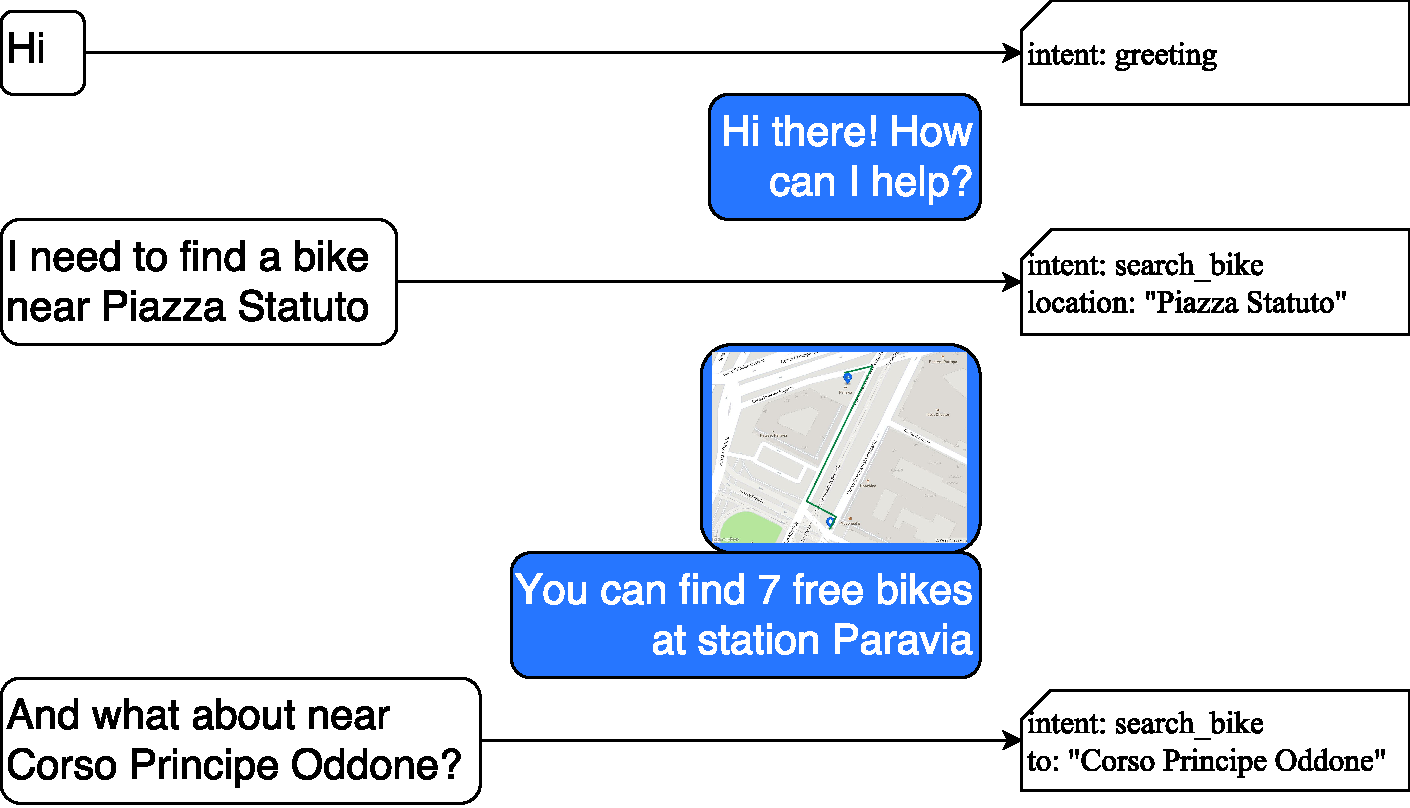
\includegraphics[max width=0.8\linewidth,max height=8cm,keepaspectratio]{figures/multiTurnImportance}
    \caption{An example of interaction where the interaction context is important for the intent classification}\label{fig:multiTurnImportance}
\end{figure}

Then Section \ref{approachPrototype} describes the approach chosen for the selected applicative prototype, by starting from the target scenarios (Subsection~\ref{approachScenarios}). A high level model is provided (Subsection~\ref{approachModel}) and then a personalization strategy is proposed (Subsection~\ref{approachPersonalization}) and the possible sources of information are described (Subsection~\ref{approachIR}). The domain is the urban mobility: the bot goal is to provide a natural language interface towards the bike sharing service. Bike sharing is one of the projects for sustainable mobility that tries to address transportation replacement especially for the so called \textit{last mile}: cover more capillary with a public form of transport areas or trips that would be uncomfortable without using a private vehicle. With respect to car sharing, bikes have much little impact on the environment and are 100\% \textit{green}. It is important to notice that not all the topics discussed in this chapter have been implemented. By comparing with the next Chapter~\ref{implementation} it can be seen that only the language understanding, the interface with the messenger platforms, the bike retrieval information and path computations have been brought to experimental environment.

Figure~\ref{fig:multiTurnImportance} shows an example of interaction in the domain of bike sharing where the previous value of the intent is important to determine the intent of the last sentence, propagating over the dialogue.

\section{NLU}
\label{approachNLU}

Before describing the NLU module, it is important to remember the approach that has been chosen: it is NLU based, not generative. For this reason the dialogue management is still done using rules and the responses are provided by filling some templates.

Without having an existing corpus to train the dialogues in an end-to-end fashion, this is the approach that best fits the situation. For example some complex rules like ``\textit{to search for a bike you should provide a search criterion or the last known position should be known and recent (2hr or ask for confirmation)}'' is not manageable from a data-only focused approach. Inside this domain, it is better to provide static rules that are handwritten in some configuration files. Although there are several studies on end-to-end goal-oriented dialog, for the implementation of this prototype a rule-based logic has been chosen. The neural network are only applied in the NLU module that is responsible to extract intent and entities from the current dialog, eventually using the multi-turn environment only to better identify intents and slots.

\subsection{Single-turn NLU}
\label{approachSingleTurn}

The computational graph that has been chosen to perform the joint task of intent classification and slot filling is the encoder-decoder model proposed in~\cite{liu2016attention} because of its State of the Art condition. By simply providing the words contained in a sentence, both the intent and the slot tags can be computed. This approach was not modified for single-turn interactions, because the performance are already good as will be seen in chapter \ref{validation}. The focus has been on how to provide better inputs to the system in terms of word embeddings and on output dependency modeling for the slot filling.

\subsubsection{Word embeddings}
\label{approachWv}

The paper presenting the used model is not describing the way the words are fed into the network. The implementation provided by the authors\footnote{\url{https://github.com/HadoopIt/rnn-nlu}} however shows that a word embedding layer is part of the model and the values are randomly initialized. Since the datasets on which the evaluation has been done is not very big (especially the ones collected for the bike sharing domain), in the approach chosen fixed word embeddings, pretrained on bigger corpora, have been used as inputs. This actually gave a little boost on performances on all the used datasets as can be seen in the next chapter. Using pre-trained static word embeddings as inputs to the neural network can help reducing the number of tunable parameters and therefore help training small corpora, in addition to other advantages, like the ability to use word-similarity also with words that were not contained in the training corpus of the domain.

This is the most language-dependent part of the network and the goodness of the classification results highly depend on the quality of the embeddings.

Natural Language Processing techniques depend a lot on the selected language and also available libraries come with differentiated support based on it. Features such as Part of Speech, or Parse Trees, if they come from statistical models or handcrafted ones, can be good only if a lot of work is done in annotation of big corpora and therefore the efforts mainly fall on the English language.

Instead approaches that consider word embeddings are less dependent on annotated corpora, since those vectors can be built by simply having sentences in the desired language, that have been computed and realised publicly on the  Web, with unsupervised techniques. As mentioned before, the bot has as requirement to support also the Italian language. Concerning English,  several preprocessed word embeddings are available, trained with different corpora and with different algorithms. Concerning Italian, the found pre-trained embeddings are \textit{GloVe} and \textit{Word2Vec} trained by the Human Language Technologies of Pisa\footnote{\url{http://hlt.isti.cnr.it/wordembeddings/}} trained on Wikipedia and the official \textit{fastText}.\footnote{\url{https://github.com/facebookresearch/fastText/blob/master/pretrained-vectors.md}}

A critical aspect to make word embeddings work at their best is to apply the same kind of tokenization both when training the word embeddings and when using them when feeding RNNs. For this application the choice has been to include punctuation in order not to discard any useful hints from the input sentences. And, hence, the two pretrained Italian embeddings have at their base a different tokenization method, removing punctuation and by applying other transformations (such as replacing hyphens and apostrophes with spaces to split the words),  the choice has been to recompute the \textit{GloVe} vectors. This time applying a proper tokenization that, as will be seen in the implementation chapter (Subsection~\ref{implementationWV}), has been applied to maximize the performance on a language that has a short representativeness in the domain-specific dataset.

\subsubsection{Output dependencies}
As mentioned in Chapter~\ref{soa}, modeling the output dependencies is very important in sequence labeling tasks. The different choices available are: feeding output labels as inputs to the decoding stage, or using a linear chain CRF. For its simplicity and also because it is mentioned in the referenced paper~\cite{liu2016attention}, the first one has been chosen.

In the description of the network in the paper it is not described how the output sequence labels are fed into the decoder. Different methods can be used: using one-hot encoding, that has the problem of scalability when the output dictionary is big enough, and word embeddings, to have a size independent from the number of existing slot labels.

\begin{figure}[!htb]
    \centering
    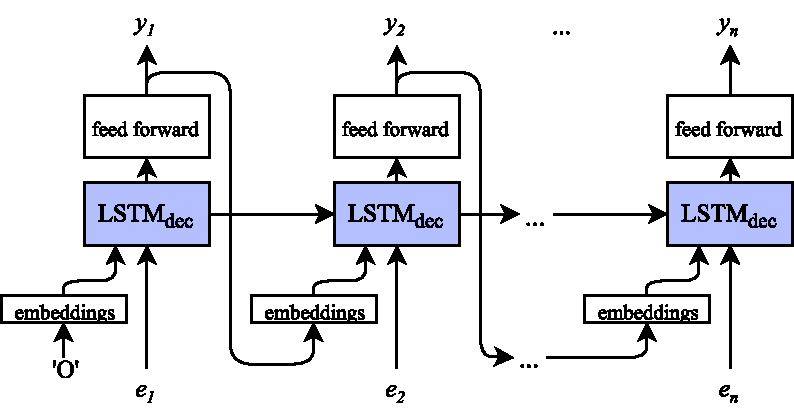
\includegraphics[max width=0.9\linewidth,max height=8cm,keepaspectratio]{figures/outputDependencies}
    \caption{The selected approach to model the output dependencies}\label{fig:outputDependencies}
\end{figure}

The choice is to use word embeddings. This time however, differently from what happens to input words, the embeddings are on a separate dictionary: the \texttt{IOB} labels. For this reason they are not used pretrained but are included as trainable parameters of the computational graph. As can be seen in Figure~\ref{fig:outputDependencies}, the embeddings values are concatenated with the current encoded word coming from the encoder. The rest of the graph does not change.

\subsection{Multi-turn NLU}
\label{approachMultiTurn}

For solving the problem of multi-turn NLU, after analyzing solutions in the literature to the problem of keeping the context \cite{xu2014contextual,bhargava2013easy,shi2015contextual,serban2016building}, the decision has been to change the single-turn architecture to consider also previous sentences. The goal does not change: classify the intent and extract the slot values. So no advanced statistical dialogue-tracking techniques are used, but the change focuses to enrich the available inputs with contextual elements to do the selected tasks on the current sentence.

The work that follows for the contextual intent classification is taken from~\cite{mensio2018multi} done for the ``Hybrid Question Answering with Structured and Unstructured Knowledge'' workshop,\footnote{\url{https://goasq.lri.fr/workshop/hqa18.html}}. Three main challenges are addressed:

\begin{enumerate}
	\item detect the change of intent in a multi-turn environment: in other words, to understand dynamically when a certain session (sequence of messages related to a single intent) ends in favour of a new one. This corresponds to choose for each input sentence whether to keep the value of the previous intent or to consider some evidence on the current input. The first case happens when the input sentence is part of a preceding session, and the user is simply continuing the interaction with the same initial intent. The second case instead is when a new intent is expressed in the current sentence, signalling an intent change;
	\item capture intent dependencies using the RNN: capturing the sequences of intent values, a better prediction of the sentence can be done knowing the proceeding intents. This can be quite useful with sentences that are not so expressive because they are referring implicitly to some context of the interaction;
	\item consider the current agent turn words: having a knowledge about what has been replied to the user can help contextualize the new sentence that may not have evident indicators of the intent.
\end{enumerate}

\begin{figure}[!htb]
    \centering
    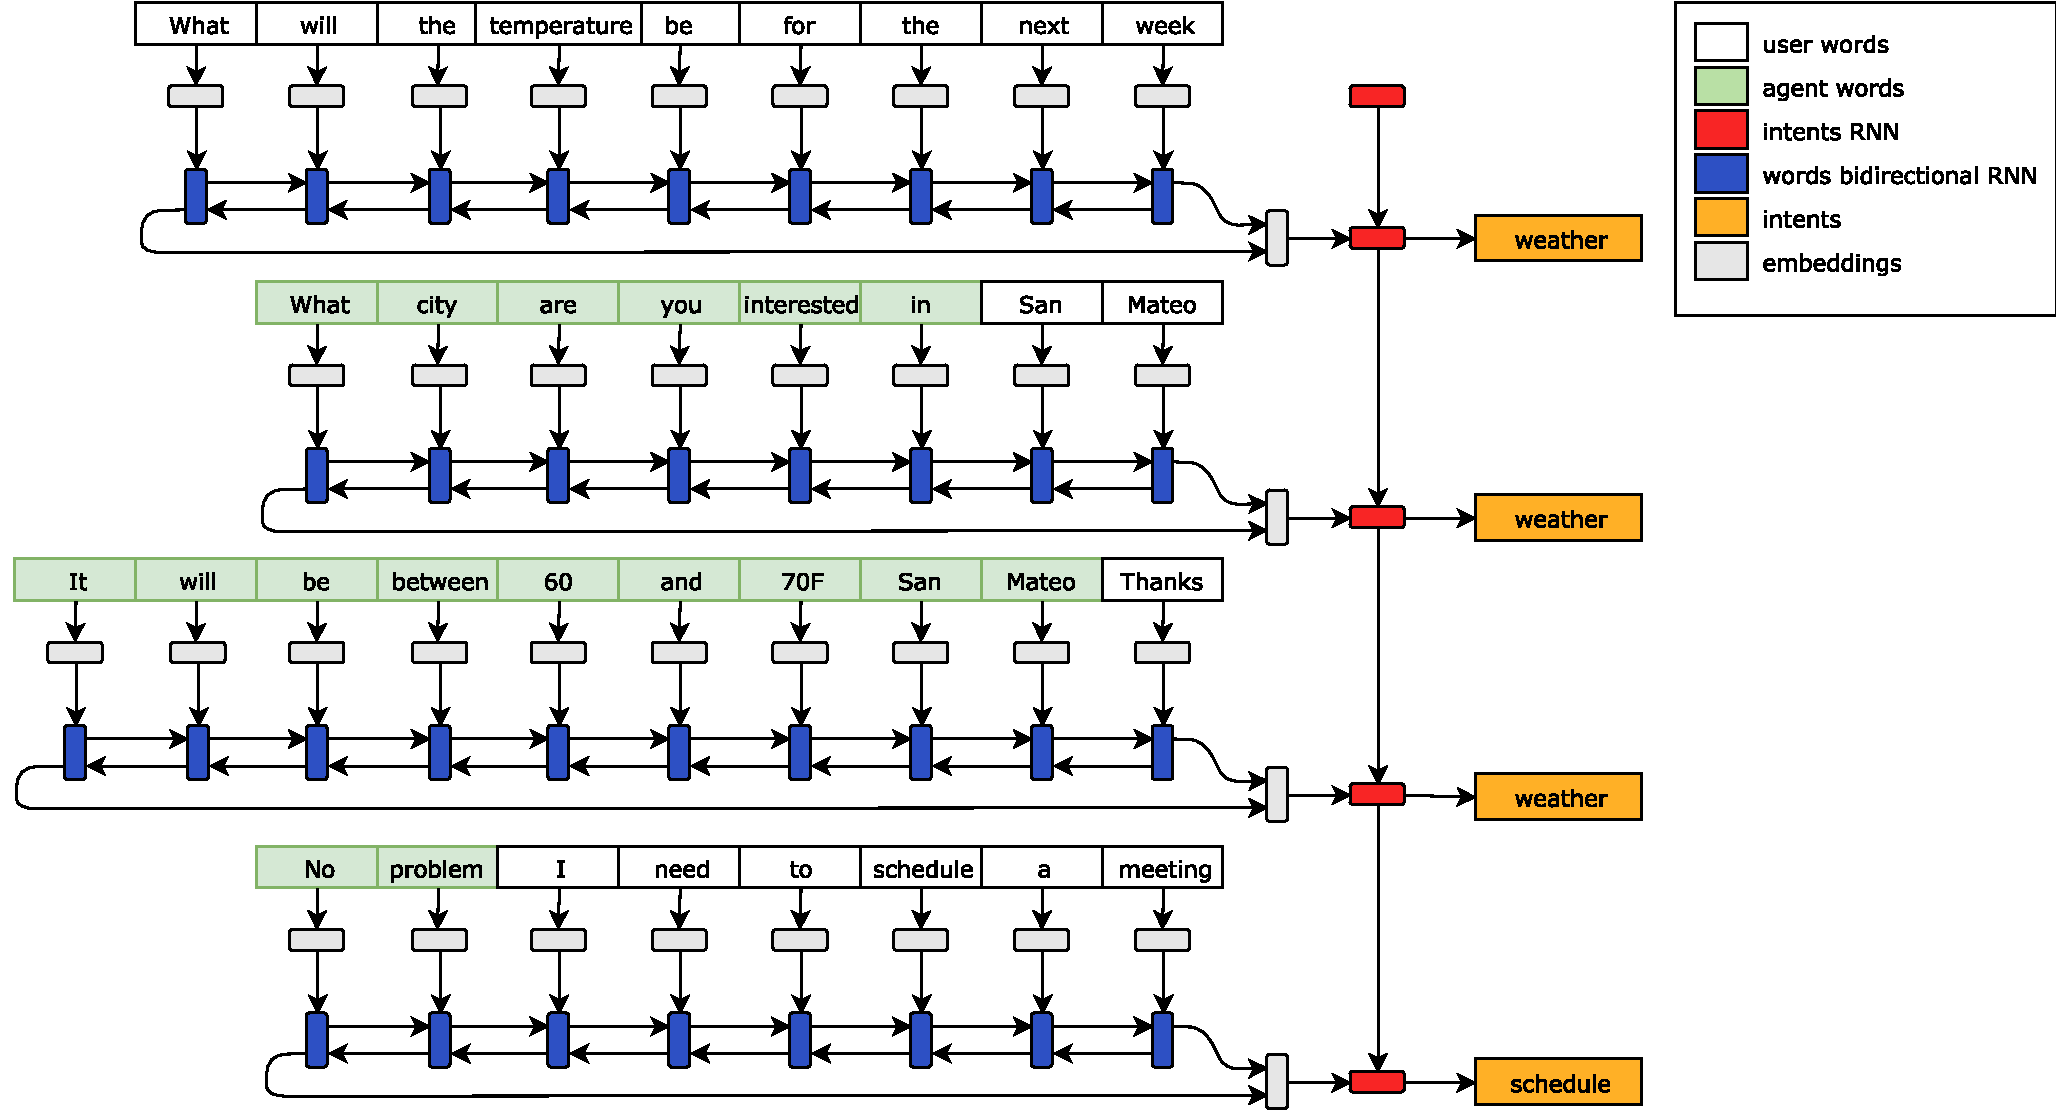
\includegraphics[max width=0.9\linewidth,max height=8cm,keepaspectratio]{figures/approachMultiTurn}
    \caption{The selected Multi-turn approach}\label{fig:approachMultiTurn}
\end{figure}

Figure~\ref{fig:approachMultiTurn} illustrates our approach. Sentences are encoded in fixed-length vectors using the word-level bidirectional RNN (coloured in blue).The outputs of this first RNN are passed to a second RNN (coloured in red) that models the intent propagation of the user sentences over the different timesteps. This last RNN (in red) for each user sentence produces the contextualized intent value. The agent words are in green, while the words generated by the human are in white boxes.

In literature also other studies have been done on the problem of sentence classification inside an interaction context. The approach proposed in~\cite{xu2014contextual} on the classification of the domain, that is like the high level class in a hierarchical intent classification, uses the previous model prediction at word-level, concatenating it with each word vector.

The approach proposed in this work is different both in the specific point where the previous classification is used (not together with the input words but on the sentence level, using the high-level RNN) and also in the way the word-level features are summarized in sentence-level features and considered for next interactions by the learning network.

A critical point where this model should prove the goodness of the chosen cell, is when two completely unrelated sentence follow each others (e.g. two different intents). In this case the LSTMs/GRUs should learn to forget their past state in order to provide the new values. In inference time we can never know whether a certain sentence is a follow-up or is a new intent without any logical linking with the previous one, so the only good option is to train the network to learn when this happens. For this motivation, instead of training on single independent sessions, all the sessions have been concatenated. In this way the model will be able to work better both on sentences that belong to the same session (for example answering back to a missing slot) and on other independent questions (for example an independent intent).

\section{The bot for bike sharing}
\label{approachPrototype}

At the beginning of this chapter the domain-specific bot has been introduced as a Natural Language Interface towards the bike sharing information.

Since there is no agreement with the bike sharing providers (with the meaning that for the majority of cities supported the only way to obtain updated data is through web scraping, not through an official API), the information is only available in read mode, and only from public sources. For this reason the main things a user can do with the bot is to ask for information on the station and availability of bikes. No account linking is possible and users cannot unlock bikes using the bot. The main idea is to provide useful information to the users in a spatial context-aware setting. To provide this, the bot should analyze the area relative to the information and provide some suggestions to the user.

A required characteristic for the bot is to support the Italian language too: the agent, being developed in Turin, is supposed to be able to understand both Italian and English. For the sentences of the agent, the solution is simply to have both Italian and English template responses. Instead for the language understanding part, as will be seen especially for the Word Embeddings in Subsection~\ref{approachWv}, it requires having the requested models for both the languages.

\subsection{Scenarios}
\label{approachScenarios}

We explain there the main scenarios that we want to face with this conversational agent. The main goal is to provide an easy-to-use interface that feels more natural for the user by allowing the interrogation in natural language.

\subsubsection{Search for bike stations information}
The main scenario is the one where a user asks for information about bikes and available parking slots. This can be expressed by a search of one station given some parameters or by a search that includes more stations.

For the first case, the user may want to find an available bike or a free parking slot given the current user position or another location. Instead for the second case, the user may want to ask for direction between two points: this involves finding a bike near the source and finding a place where to leave it near the destination.

The system, given simple queries expressed in natural language, should understand the request and extract the necessary parameters. The retrieval of information should include the interrogation of the bike sharing system or using cached versions, with the aim to find a path for the user that follows the constraints specified by the user and by the bike availability. Other sources of information that may be consulted are weather information (to provide alerts for the given location) and routing information in order to return a path that can be used by bikes.

The history of conversation is stored in a way to find temporal and spatial pattern for the user, in order to build a model that can be used for personalizing his experience for example by providing places suggestions, as will be seen in Subsection~\ref{approachPersonalization}.

If there is a place that can be suggested, with sufficient confidence of the recommending systems (telling that the suggestion is appropriate and relevant), additional information about it can be included in the response that is generated.

Such response should have the form of natural language, with the possibility to include visual contents such as pictures or links to more detailed information about the results.

\subsubsection{Search for supported cities}
Another scenario is when a user wants to understand the availability of the information for a specific city. In this case the request, expressed in natural language, will contain the name of the city. The system extracts it and finds if any bike sharing providers have support in it. If the city is not supported, information about which nearby locations are supported can be provided in the response.

\subsubsection{Small talk, refining the user model}
The last scenarios is the one of small talk: all the sentences that are not necessary to provide information about bikes, but are necessary to handle very basic chit-chat dialogues.

The user may use greetings, generic responses like yes/no, questions about the bot and other sentences that can be easily replied to, just to make it seem more natural.

Knowing that user expectations can be easily destroyed with a ``\textit{I don't understand}'', some answers have been added only to mitigate a very big problem that still is present and could only be solved with generative approaches.

Having some dialogues of this genre with the user could help understanding more about him, and this kind of information could be useful for refining the personalization model. By having a mixed-initiative interaction instead of letting the system to reply only to the questions, the bot may also ask questions to the user about his interests or explicitly asking for some feedback. In this way the personalization would receive a boost.

\subsubsection{Proactive messages}
Extending the mixed-initiative interaction out of the single dialogue, the bot may be able to actively begin the conversation with the user after some time of inactivity (not possible to start conversations with new users of course). This can be seen as breaking the idea of the bot as a service and for this reason should be only done if there is an advantage for the user. The advantage can exist in two different situations.

The first one is when, after having provided some kind of information to the user (e.g. a bike is available in a specific station) and before the user arrives there, the situation changes (e.g. the bike is no more available or the weather is getting worse). In this case the bot could actively send a message to the user informing about the change.

The second situation is when a pattern in the behaviour has been observed (e.g. the user always searches for a bike at 8am in a fixed location). The system (some minutes before the forecasted event) can send an unsolicited message to the user informing him about the bike availability.

Those messages must be in some way controllable from the user. The suggested way of making them available is to test them once on the user and then getting the feedback: if the user reacts positively (measured by explicit response or interacting with the generated content) the feature can be kept on, otherwise the system will remember not to use the feature with the current user.

\subsection{High-level model}
\label{approachModel}

Given the main scenarios and given the fact that no publicly available corpus exists for the selected domain, the choice of the approach could not be in favour of an end-to-end system with dynamic response generation, but towards a NLU-based understanding. About the Information Retrieval, the data comes from external fixed set of APIs so it has been chosen to keep this approach instead of turning all the information in explorable graph of connected entities. These choices, together with the delineed scenarios, require the presence and cooperation of different components.

\begin{figure}[!htb]
    \centering
    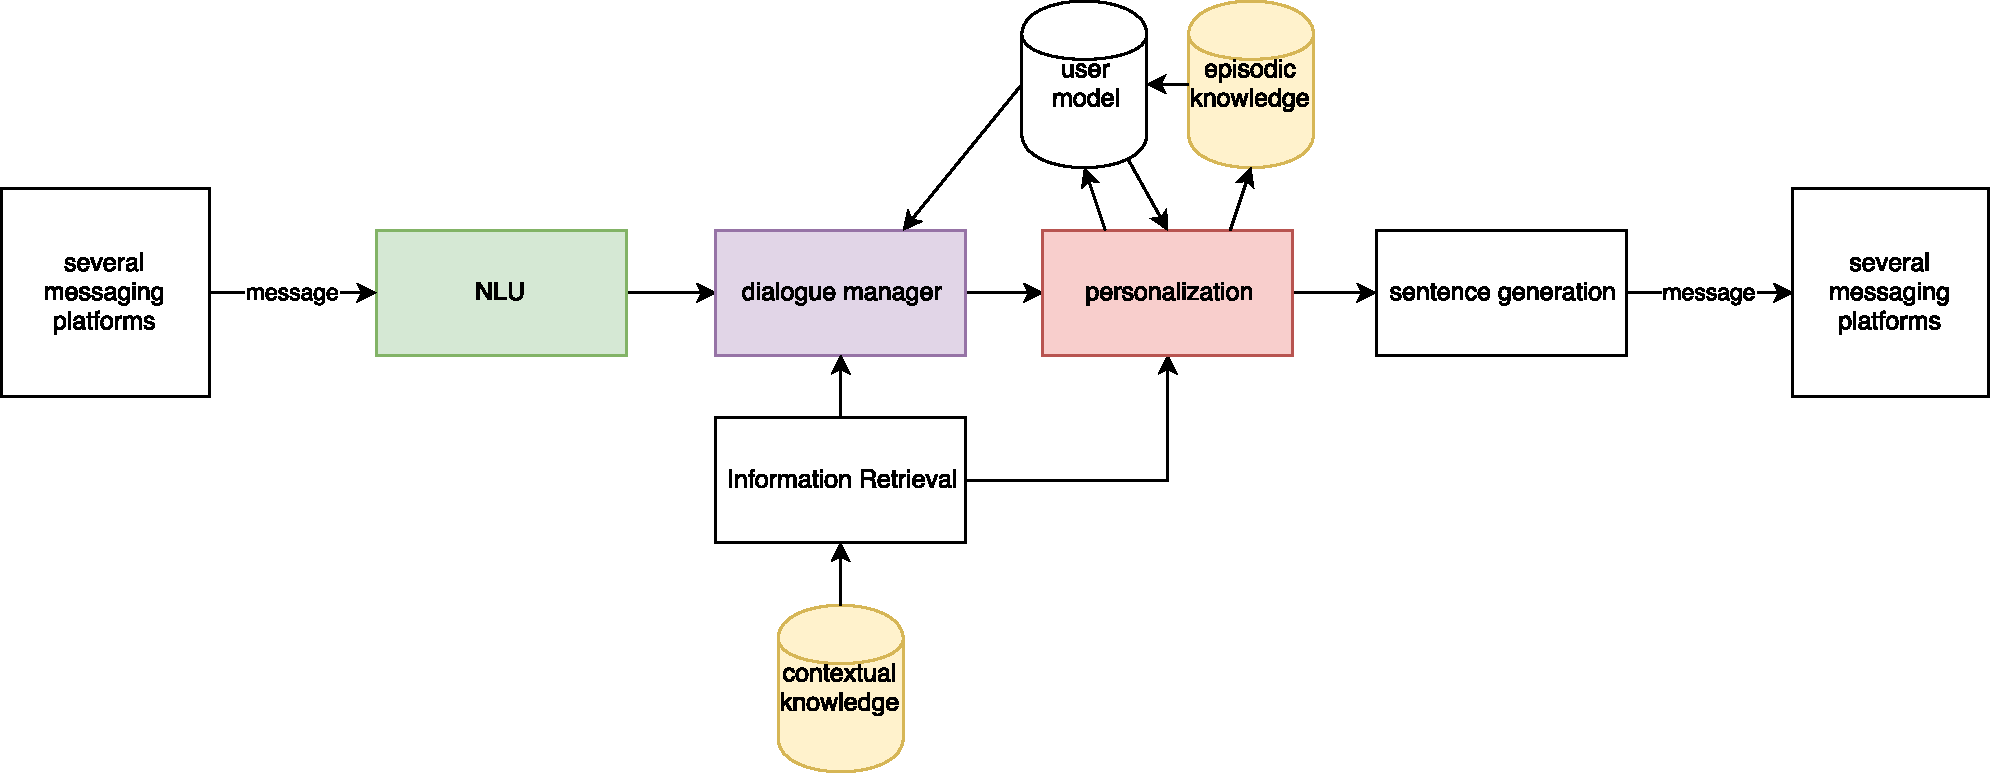
\includegraphics[max width=0.9\linewidth,max height=8cm,keepaspectratio]{figures/systemHighLevel}
    \caption{The high level model of the system}\label{fig:systemHighLevel}
\end{figure}

As can be seen in Figure~\ref{fig:systemHighLevel}, one component is needed to interface with the different messaging platforms. This is responsible to make messages arrive to the ``brain'' of the bot and to deliver responses back. Something about this component will be described soon and some implementation details will be given in the next Chapter (Subsection~\ref{implementationInteraction}). Then another component will do the NLU, providing intents and resolved entities. Passing through the dialogue manager, that contains the rules for managing the conversation, the flow will reach the personalization module that will collect episodic knowledge and together with the contextual knowledge will provide recommendations. The responses will be generated by combining the results and some templates will be filled.

The main sources of information (knowledge base) can be grouped together in two types: the Contextual and Episodic. In the first group can be found the providers of information, that are used in read only mode, inherent to bike sharing, places, weather. The data is provided by external web API, and may be cached locally for performance improvements. The Information Retrieval module is responsible to manage them providing a higher level API that can be easily used by the dialogue manager. Instead the Episodic Knowledge contains records captured from the interaction with the users. Aggregated information can be computed and put in the user model that collects the user features that can be used for the personalization.

Going a bit deeper on the source and destination of messages, we are discussing about the messaging platforms where chatbot can be created. Nowadays there are so many different options available and every one of them has different features. There are even some of them that do not allow bot users. For example, the most widely used chat platform WhatsApp strictly forbids non-human accounts, punishing with permanent banning.

Starting with one of the first platform to support bots with official API, Telegram Messenger is surely the easiest platform to create bots on, allowing them since June 2015. Bot accounts can be easily created in few seconds with the only principle that the username should end with ``bot'' in order to be recognizable. User can interact with bots using text, voice, buttons of different kinds, images (any kind of file can be sent) and including them also in chat groups. On mobile devices users can also send their location. This platform is the most friendly for bots, but is not widely used by non-geeks.

A very commonly used platform is Facebook Messenger, that opened to bots in April 2016. This platform is widely spread because is part of Facebook, and is available for every devices, also from web browsers. On Facebook Messengers the features are text/voice exchange, buttons of different kind, images and even attaching the user location. Facebook Bots have their Facebook Page and a few configuration steps need to be done to be able to set up a new bot. Other chat platforms that allow bots are Skype, Slack and Kik.

Other interesting communication channels are arising with expandable virtual assistants, that focus more on the use of the voice. Expandable in the sense that developers can develop some abilities for some domains and users are allowed to select them and add to the behaviour of the virtual assistant. We are talking about Alexa Skills and Cortana Skills. For these platforms the interaction with the user is quite different because instead of communicating directly with the user, the virtual assistant manages the conversation.

There are so many different platforms that it would be quite restricted to focus only on a single one. Furthermore the APIs change a lot between them, and even between different versions of the same platform.

Since all the details of the API are only an implementation detail, that will be fastly covered in the implementation chapter, here we will give only the motivation that lead the design of the system to be split into two parts: one will manage the channels and communication from and towards them, while the other will handle the important conversation stages (comprehension with NLU, dialogue state management, information retrieval, personalization). The message exchange between the two parts is done using a neutral representation, not dependent on any of the destination platforms.

This is what is intended with the term \textit{Multichannel Support}: the core of the chatbot can be put in communication with any messaging platforms, given that the message-proxy component (the part of the two that depends on the specific platform) is correctly configured. This component can make use of one of the many available solutions to manage different channels: Microsoft Bot Framework, Recast.AI Bot Connector, or start from scratch the implementation of the different endpoints. As will be seen in the next Chapter (Subsection~\ref{implementationInteraction}), having this component has many practical advantages.

\subsubsection{Intent and slot types}
\label{approachTypes}

From an analysis of the scenarios, an hypothesis of the common user intents has been done, and from them also the slot types have been modeled. Intent and slot types have been successively refined in successive iterations by observing the transcript of some test users.
The intents that have been used can be seen in Table~\ref{tab:nluTypes} together with some examples.

% !TEX encoding = utf8
% !TEX root = ../main.tex

\begin{table}
  \begin{tabularx}{\textwidth}{lXX}
    \textbf{Intent type} & \textbf{Example} & \textbf{Slots} \\
    \toprule
    \texttt{search\_bike} & Find me a bike near Central Park & \texttt{LOCATION('Central Park')} \\
    \midrule
    \texttt{search\_slot} & Where can I leave the bike near Big Ben &\texttt{LOCATION('Big Ben')} \\
    \midrule
    \texttt{plan\_trip} & I want to go from Piazza Castello to Porta Susa & \texttt{FROM.LOCATION('Piazza Castello') TO.LOCATION('Porta Susa')} \\
    \midrule
    \texttt{city\_supported} & Is Torino supported? & \texttt{LOCATION('Torino')} \\
    \midrule
    \texttt{set\_position} & I am in Rue de France, Nice & \texttt{LOCATION('Rue de France, Nice')} \\
    \midrule
    \texttt{ask\_position} & Locate me & \\
    \midrule
    \texttt{booking} & Please book me a bike near Piazza Navona & \texttt{LOCATION('Piazza Navona')} \\
    \midrule
    \texttt{greeting} & Hi there! & \\
    \midrule
    \texttt{info} & What can you do? & \\
    \midrule
    \texttt{end\_discussion} & Ok & \\
    \midrule
    \texttt{thank} & Thank you! & \\
    \bottomrule
  \end{tabularx}
  \caption{Intent types and examples}\label{tab:nluTypes}
\end{table}

While the intents, once recognized, are ready to be used in a rule-based logic (each intent is linked to a set of actions that must be performed), for the slots more work needs to be done. First of all a check of the required ones based on the intent type, providing some questions back to the user to request them when missing. And then another component, the \textit{entity resolver}, needs to translate text spans into living entities. For the entities of type \texttt{LOCATION} this corresponds to translating a text into a location object with latitude, longitude, full name.

During the progress of this task many problems can arise. First of all, the user may refer to some place names that are bound to a position only for them: examples are ``home'' ``work'' and ``school'' that are different for each user. For this reason this type of resolution and memorization is required to be personalized. Another common problem is the disambiguation of places with the same name that exists in different contexts. Geocoding can be biased on a specific area to give a preference on a certain bounding box,\footnote{\url{https://developers.google.com/maps/documentation/geocoding/intro\#Viewports}} but the identification of this box is itself a problem because we can never know if the user is visiting some unusual places.

Apart of all those problems, the chosen solution is to use third party geocoding services to translate from a place name to a structured object that enables to work with the latitude and longitude to provide the desired path information. The problem of disambiguation and personalization are kept for future works.

The entity of type \texttt{LOCATION} can be inside the utterance as entity or can be the user position. Other entity types have not been considered for this initial prototype.

\subsubsection{Dialogue State Management}
The Dialogue State Management module is responsible to handle the mapping from intents and available slots to the actions and responses. For this part, as mentioned before, a rule-based approach has been chosen.

Each intent type is mapped to a specific set of actions. Additionally for each slot type that is used in a certain intent type a rule is configured to say if it is compulsory to have a value or not. In the case the slot is compulsory, the Dialogue State Manager must ask back for it, prompting a question to the user.

The intents that have been designed however have another type of rule: the location entity can be replaced by the current position of the user, that can be sent as attachment or expressed with the corresponding intent \texttt{set\_position}. If the value of the user position exists and is recent (last 2 hours), it can be used. Otherwise the user is required to provide it.

Once the requirements have been checked, the corresponding actions are called, involving the interrogation of the bike sharing information and other collateral sources. At the end, when the results are ready in a structured format, the translation back in natural language is done by filling some template responses with some item features.

\subsection{Personalization}
\label{approachPersonalization}

This section explains how the personalization techniques can be applied to the interactions with a chatbot, providing personalized content recommendations in a tailored communication fashion. This approach is composed of two main parts: \textit{content recommendation} and in this specific case the contents that are provided as recommendations are places around the user that he could be interested in. The second part is relative to the \textit{interaction itself}: the goal is to change the behaviour of the bot relatively to the mood of the user, in a dynamic way.

It is very important to notice that the topics here discussed have been used in a design phase but they have not been developed and tested. However we kept this section as part of this work because its content can be used for future studies (as discussed in Chapter~\ref{conclusion}) that may implement the idea represented here. Furthermore, not only a personalization approach is presented, but also a bit of analysis of third party information providers that could enable this scenario, such as Facebook Graph API or Big Five predictors (in Subsection~\ref{approachIR}).

\subsubsection{Content recommendation}
\label{approachRec}

For giving content recommendations, the objective of the recommender is to provide interesting places for the user around his trip. The area of search is therefore established by the results of the information: different strategies could be used to determine this surface, but the fastest one, that helps also querying providers of places information (e.g. Foursquare, Facebook Places, Google Places), is to use a circle determined by its center. As can be seen in Figure~\ref{fig:placesSearch}, the circle is centred in the mean point between the source and the destination, while its radius is chosen to cover the source and the destination plus an additional margin. The margin enables to provide also some places nearby the source or the destination that would be clipped out otherwise.

\begin{figure}[!htb]
    \centering
    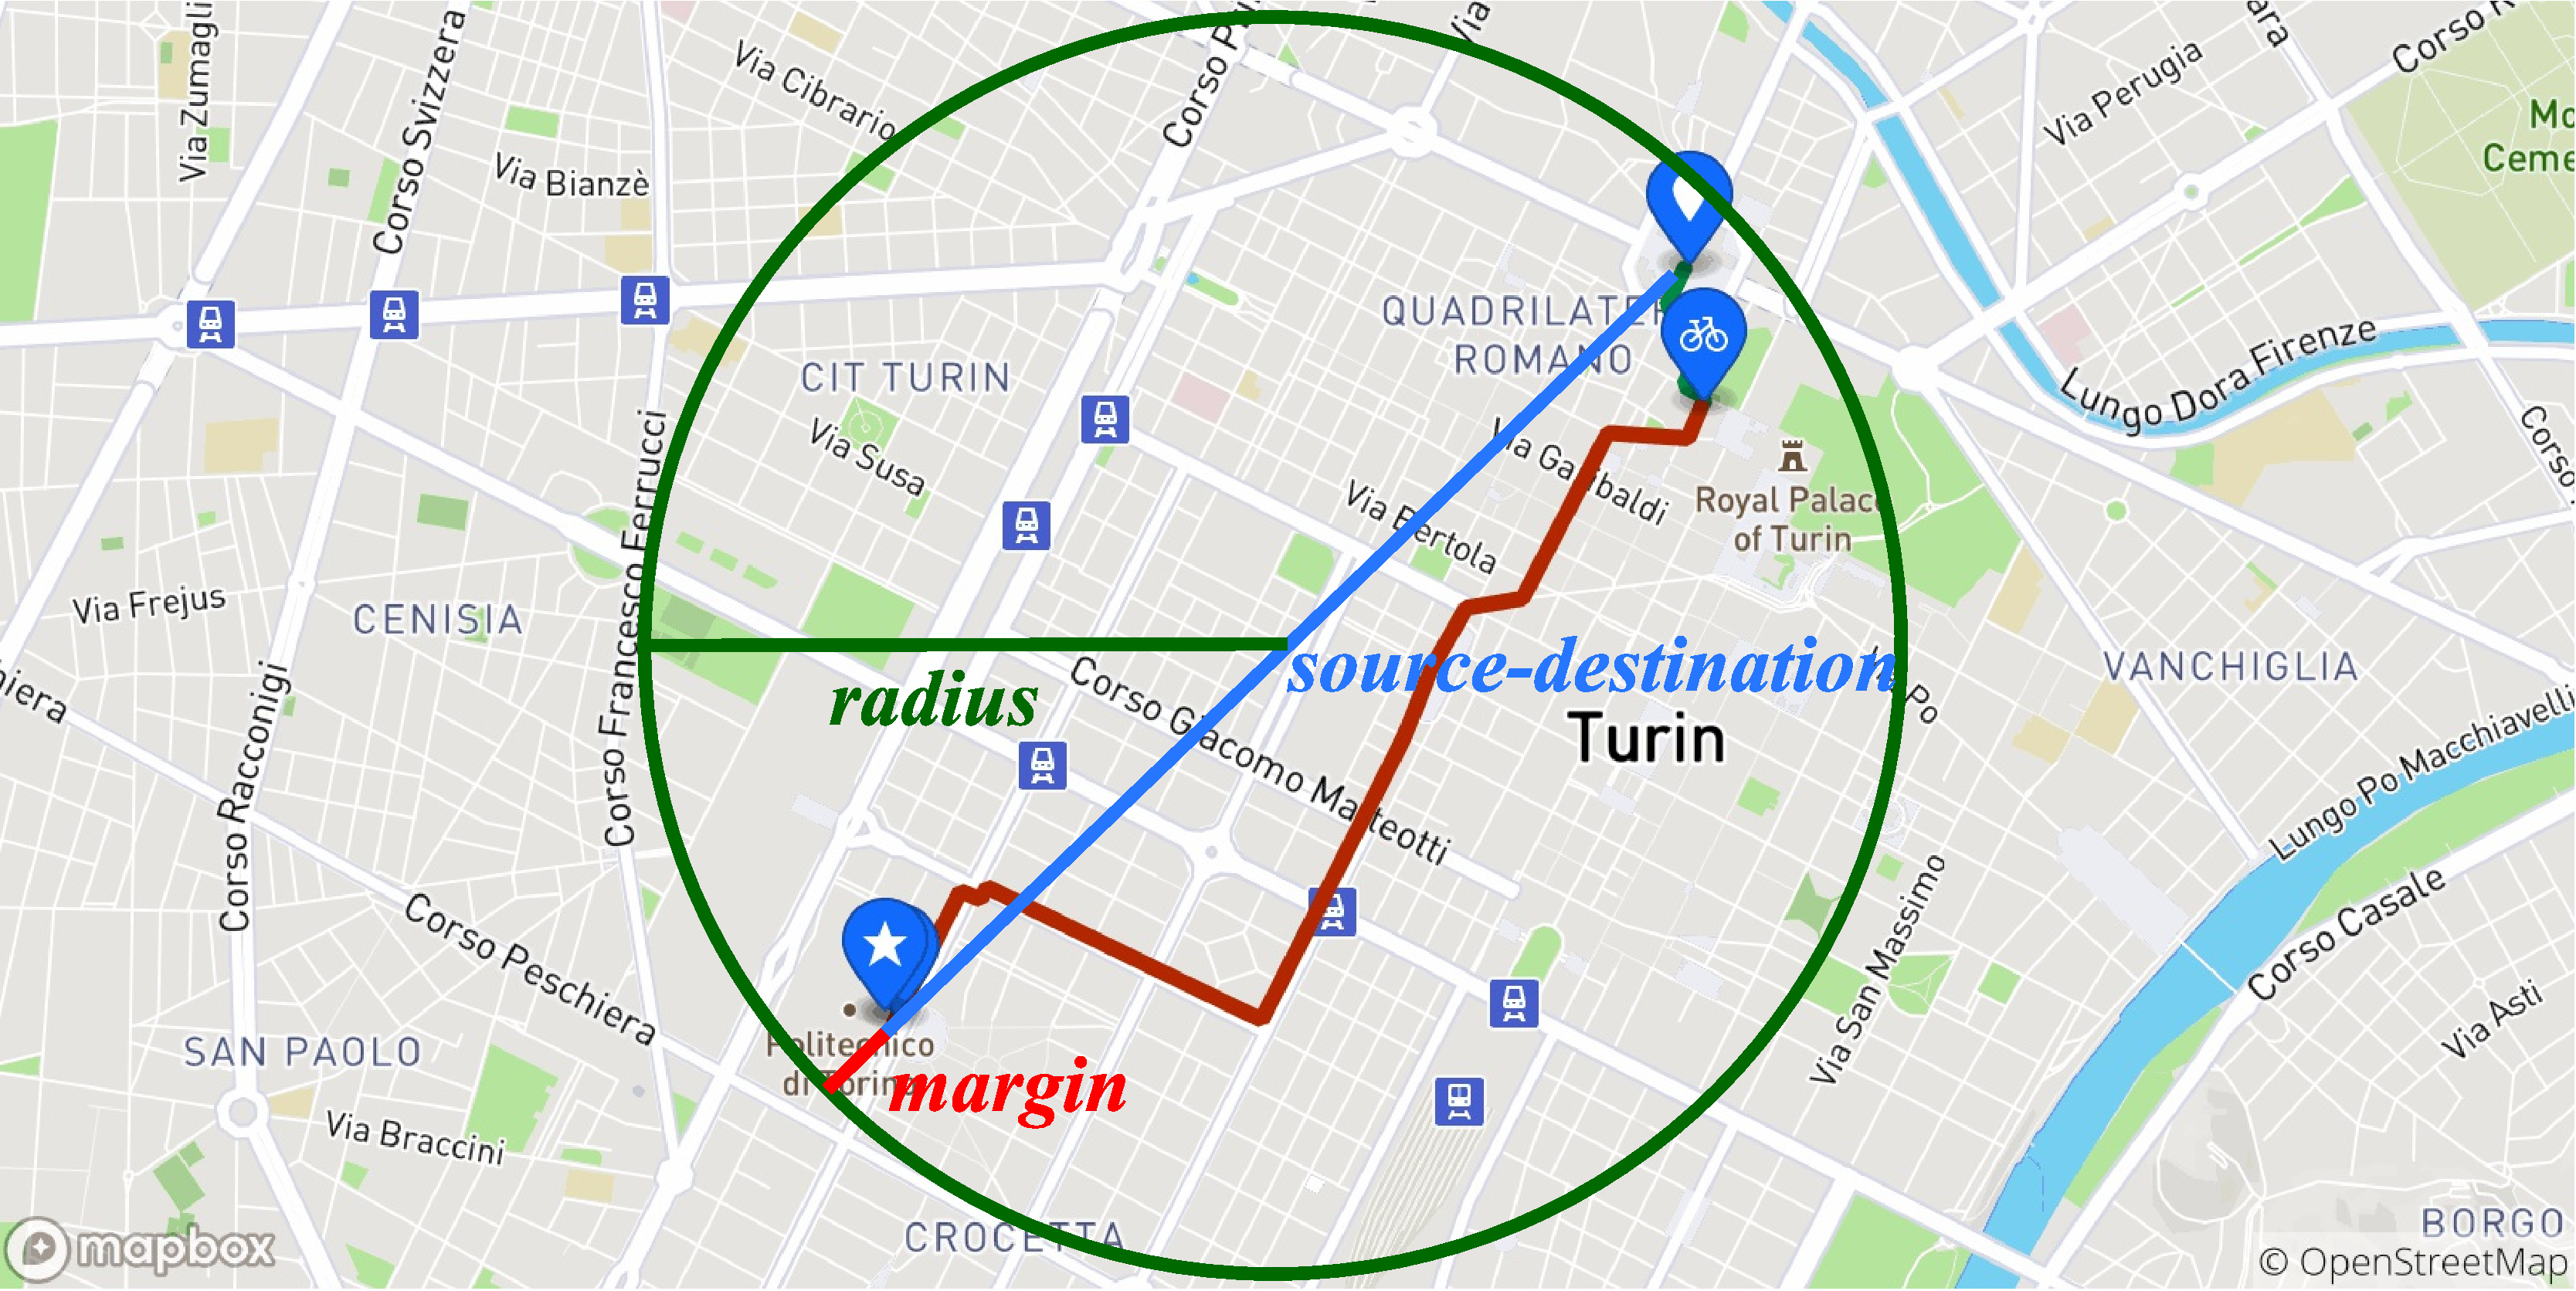
\includegraphics[max width=0.9\linewidth,max height=8cm,keepaspectratio]{figures/placesSearch}
    \caption{The geographical constraints to search places for the recommendation}\label{fig:placesSearch}
\end{figure}

Determined the valid surface, the places in it are candidates for the recommendation. To restrict the places list and to provide one of them as recommendation, the strategy to be applied is to determine a place category that the user could be interested in. To find this category, a bit of user modeling needs to be done.

\paragraph{User modeling}
First of all, it is important to understand which variables need to be collected to build the user model. Some manifest variables like gender, age, profession, religion, political orientation are used for many profiling techniques, but not always they are available. Moreover, from a bot that is giving bike sharing information it is strange to be asked for those values, and can only make the user stop using the bot because it is asking strange questions. For these reasons, this kind of information is not even asked to the user.

As explicit data collection, some questions can be asked to the user in a more appropriate way, relatively to bike sharing. For example asking why the user makes use of bike sharing: to go to school, work or simply to run errands around the city. Having a general knowledge of the main purpose of using the bot should be really helpful, extracting personal details like occupation or student status. This type of information can be collected at the beginning as bootstrap questions, or also after some dialogue with the user has been done. In this way the user can soon use the service without being blocked by bootstrap questions, but after some minutes of inactivity he can be sent some questions in order to improve the service. In any case, waiting for responses should not block in any way the understanding process of new requests. For this reason it is important that the classification of intents continues to work, distinguishing dynamically if the user is keeping the discourse in the bootstrap environment or if he is providing his own intent to reach some details about bike sharing. 

Other explicit information can be collected when the recommendation is in act, as feedback to the suggestions: feedback can be positive or negative, collected through specific buttons or intercepting the user clicking on the information given about the place. The feedback can help refining the user interest and also understanding his attitude towards recommendations (as will be seen in Subsection~\ref{approachPersonalizationCommunication}).

As implicit user modeling, observing the patterns (temporal and spatial) of the queries performed can help find users similarity and improve the collaborative filtering approach (as will be described soon). The patterns in the spatial dimension correspond to frequent places, while in the temporal dimension can be interpreted as habits.

Other optional sources of data may come from social networks. On social networks people usually show their interests towards different kind of things: check-ins, places, music, films, and many others. This can be very helpful to user modeling, both providing user features both providing item (places in this case) features. The inputs in this case are the interests of the user, that can be provided by doing a login on the desired social network. The access scopes\footnote{\url{https://developers.facebook.com/docs/facebook-login/permissions/}} usually can be requested with different granularity levels and allowing different types of personal information to be retrieved. This login is proposed to the user as optional and if denied must not preclude any functionality of the bot. Simply the model for this user will not be accurate and more generic recommendation will be provided.

Given the social network footprints, a prediction of the \textit{Big Five personality traits} can be done using some online available APIs (see the related Information Retrieval description in Subsection~\ref{approachIRbig5}): the user features will be the \textit{Big Five} together with \textit{concentration} on different areas (like art, biology, business, IT, education, engineering, journalism, finance, history, law, nursing and psychology). These features try to describe the personality and the possible interests of a person, and can be computed easily as will be seen in the section. Furthermore, as described previously in Subsection~\ref{soaPersonalizationFeatures}, they come from expert psychological studies~\cite{costa2008revised} and are proved to be able to predict unpublished user features~\cite{kosinski2013private}.

Once these user features are collected, different recommendation paths have been modeled to suggest the categories of places inside the selected area.

\paragraph{The trainable relationship}
The recommendations of categories are given following an hybrid recommendation approach, combining content-based with collaborative techniques. As can be seen in Figure~\ref{fig:recommendationPaths}, there are different entities involved, but the main goal is to learn the mapping from user features to place categories. This is the unknown relationship evidenced in red in the figure. The model needs to retrieve as many details on the two edges of this relation, in order to be more able to suggest the best places for each user.

\begin{figure}[!htb]
    \centering
    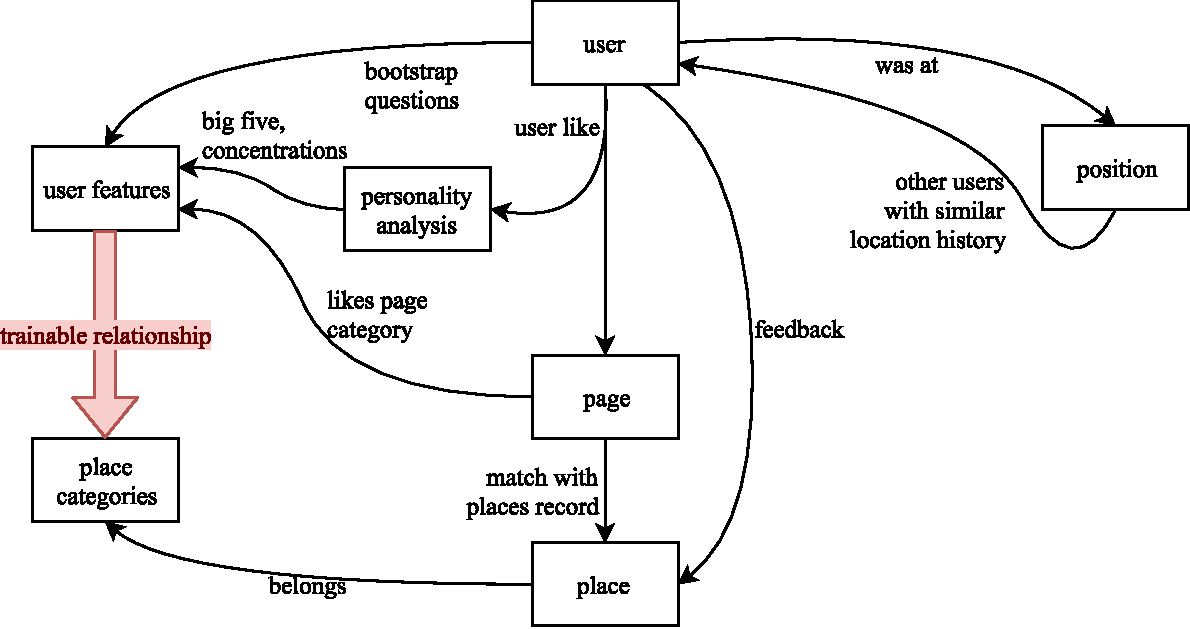
\includegraphics[max width=0.9\linewidth,max height=8cm,keepaspectratio]{figures/recommendationPaths}
    \caption{An overview of the possible recommendation paths between the user and the places}\label{fig:recommendationPaths}
\end{figure}

There are different ways to collect the details of user or of the places. The user features have just been described, but to have a correlation between them and the places features, it is necessary to collect also information on the other side of this trainable relationship. For this reason, when connecting to third party social networks (gold candidate is Facebook), the desired scopes for this personalization strategy should allow exploring the user interests (Facebook \textit{Likes}) and the places where the user checked-in (similar to the Foursquare checkins, Facebook calls them as \textit{user tagged places}). The first ones, besides allowing to infer user features, allow exploring the places he likes, because pages can have a physical location. The places that have been visited or have been ``liked'' by the user can be used to analyze the respective categories, and add training data.

Yet another input can be used to feed data about this trainable relationship: explicit and implicit feedback. Receiving signals from the user about a recommendation, the model can be refined depending on the positivity of the user opinion. The explicit feedback is acquired when the user evaluates the solution, and the implicit can be collected by using a link rewriting strategy that captures when a suggestion link is visited.

All those inputs are used to train this relationship that models how different users with similar interests are likely to appreciate places with similar features. To model this unknown mapping, a simple feedforward neural network can be used and trained with the data of every user. It is a content-based component because users that have expressed a positive opinion on a certain category, will receive recommendations with places that have similar characteristics. But it is also collaborative because the relation is trained with data of all the users, so similar user features map to similar places features.

\paragraph{Providing recommendations}
So given any user and any constraining circle around his path, different recommendation strategies can be applied depending on which inputs are available.

First of all, the trained relationship can be exploited if enough inputs are known. This is the case where the user has done the social login and/or has provided answers to the bootstrap questions. Using his feature vector, an estimation of the categories he is interested can be done by applying this hybrid recommendation component. Once the categories are found, the search within the bounding circle can be performed by giving preference to them.

If the user feature vector is not yet populated, or the previous recommendation strategy gives results that have low confidence, another strategy is to use the explicit feedback provided on previous recommendation. This time, no hybrid recommendation is used, but only a content based one, suggesting places with a similar category to the ones that were previously appreciated.

If also this kind of information is not available, but the user has used the bot for a while receiving several times path directions, another strategy can be applied. The idea is that users with similar spatio-temporal usage patterns are somewhat similar, because they go to the same places around the same time. Following this idea, an analysis of those patterns can be done by applying some unsupervised techniques, such as user clustering based on the Episodic Knowledge. The features to include for this clustering are time and space of the locations involved while performing the interaction with the bot. As output from this application of clustering we can get a neighborhood of the user in this space of spatial and temporal features. We can then use the identified similar profiles and ask the recommender a suggestion with respect to them, and see the effect of propagating this recommendation to the starting user. This technique is therefore really collaborative.

However all those strategies rely or on a properly featured user (to use his feature vector), or on a wide usage by different user (to enable the neighborhooding search). Those aspects are heavily suffering from the cold start problem. To mitigate this effect, especially on the first epochs of the system where a very limited number of users are interacting with it, a last technique can be used. Places API, as will be seen in the section relative to the Information Retrieval \ref{approachIR}, usually provide a section named ``trending places'' (in the jargon of Foursquare they are called \textit{top picks}). This kind of places usually represent very interesting places in general, that can be safely suggested to the new users. An important role again is played by collecting the feedback after prompting the suggestions. Generic recommendations can be given at the beginning and can be slowly refined by collecting the feedbacks and collecting more users that hopefully will accept to perform the social login.

When a certain distribution of probability over the place category is computed, there are still some choices that can be performed to reinforce the recommender system. One of them, typical of the reinforcement learning, is the \textit{exploration vs exploitation dilemma} that in this case can be seen as: it is better to provide an experimental suggestion that has a low confidence score and could result both in a serendipitous acceptance and brutal rejection, or to provide a more confident suggestion that can be seen as foregone and will not help discovering more about the user? 

To put this dilemma into action, an $\varepsilon$-greedy~\cite{tokic2010adaptive} can be used to dynamically determine a \textit{temperature level}~\cite{hinton2015distilling} that will model the softmax smoothing. A low temperature value makes the recommendation more confident and stays on the exploitation side, while an higher value tends to make the choice over the categories more random, on the explorative side.

If this approach is implemented, measures of its goodness should consider not only the accuracy of recommendations, but also their diversity and serendipity.

\subsubsection{Tailored communication}
\label{approachPersonalizationCommunication}

How introduced previously, we think that the personalization strategy in a textual environment should not be limited to content recommendation. Being human conversation itself one of the most dynamic interactions where it is very important to understand the interlocutor to say the things in the right way, in the following paragraphs different modifications to the mean itself of interaction are considered. First of all, some operative modes are defined to represent different behaviours with respect to the recommendation process. Then a memory of the personal preferences, letting the bot remember things that can be useful to fasten the interaction (having places saved with names like ``home'' and ``work''). And finally some considerations that can help reducing the linguistic style distance between the user and the bot.

\paragraph{Operative Modes}
Starting from the operative modes, we can define them as states of conversation that model how much the recommendation process should be active and visible to the user. It should reflect how much the user is willing to receive suggestions relatively to interesting places in addition to the normal information about the trip.
Three operative modes can be designed:

\begin{description}
	\item[Normal:] the recommendation are provided when the system is sufficiently confident. This means that not for each search a recommendation is provided, because that would be too much, but sporadically a place is suggested and the effect on the user is observed;
	\item[Straight to the point:] the user expressed negative sentiment in response to a recommendation, or may be in a hurry and needs only the bike information. In this situation, the bot is not allowed to send recommendations because can lead to a very negative attitude and abandonment of the conversation;
	\item[Conversational:] the user is chatting with the bot, asking some questions about it. This may be the right moment to ask some information to the user in order to refine the model. Questions should not be too personal, but always somewhat related to the topics discussed. An analysis of the personal interests can be done to understand better which categories can be interesting for him.
\end{description}
To decide which operative mode should be applied, it is very important to collect signs from the users. Signs can be explicit in feedbacks: both textual or by using some buttons next to the results. Signs can also be implicitly sent in text messages: latent sentiment analysis can sometimes provide sporadic hints.

Or signs can be collected from monitoring the destination pages that are linked in the results. For this reason the strategy of link rewriting can be used to intercept the user clicking on the details of the recommendation: an intermediate webserver can be set as the destination when creating the link; when it receives the request, it records the fact that the user has reached it and sends a redirect for the real destination. This strategy is widely used to measure click-through rates by all the big companies (see for example the real URL used in the results of a Google Search, or the links built by Facebook and Twitter).

\paragraph{Personal preferences}
The personalization, beyond providing the recommended content in the correct way, should also consider some personal preferences that may enable a faster and more comfortable usage, like setting bookmarks or saving form fields in a web browser. In the domain of bike sharing, it can be useful to let the user save favourite stations, linking them with a shorter name, or saving the values for other commonly frequented places, like the home or the work/study location. By having this personal map between names and locations, searches can be performed faster and without the need to remember long addresses every time.

Other preferences that can be saved for the bot, are values that play the role of settings: set automatic messages in certain time slots, to receive unsolicited messages for bike availability on recurrent habits or to receive constant updates about a bike station in the minutes before its usage. Those are all things that could enhance the user experience.

\paragraph{Linguistic style and mood}
Furthermore, the personalization strategy could also be expanded to the linguistic style of the user. This can declinate on a targeted choice of language or the usage of emotions. Those enhancements can be used effectively only if responses are provided in a generative fashion.

On the choice of language, what can be done is a imitation of the formality level and jargon. This is what happens in real life dialogues, where the terms people choose are usually targeted to the interlocutors and the sentences are generated to fit the social situation. In a generative approach, as works like~\cite{li2016persona} show, the language can be modified by being more user centric with respect to speaking style, that can reflect also some background information of the interlocutor.

Instead on the side of emotions, as~\cite{zhou2017emotional} shows, the output of generative approaches can be biased on a specific emotion. This can help making the user more understood by reflecting his mood of writing. However, as discussed in the introduction, this emotional content has many potential negative effects on the personality and should be evaluated well in ethical field before giving any implementation.

\subsection{Information Retrieval}
\label{approachIR}

This subsection analyzes the kinds of information that both have been used in the prototype and may be used for the implementation of the personalization approach. Some details are given about each data source that is necessary, together with the respective APIs that can be used. The sources of data cover different domains: from the bike sharing information, passing through the computation of directions and geocoding, and going in the direction of personalization by means of APIs to retrieve the recommendation items or APIs to compute user features. Below are listed the different data sources that need to be queried to provide updated information to the users.

\subsubsection{Bikes}
Bike sharing is an expanding market, where every day more companies are investing in and more people decide to use them for their relatively small cost and for their easiness in the urban environment. The majority of the providers have station-based systems, where the users begin and end their trip at fixed locations (the stations). However nowadays station-free systems are being spread in major cities, with the advantage of being able to leave the vehicle in any responsible place.

Given the multitude of companies and the economic competition between them, and also the fact that in different cities multiple providers are available (e.g. in Turin there is the station-based toBike and the station-free oBike and MoBike), interfacing with them is quite difficult for two reasons:

\begin{itemize}
	\item The bike sharing providers may not want to make available their data to third-party players, both for privacy issues (data disclosure can be quite a problem also in this domain\footnote{\url{https://www.cnet.com/news/yellow-bike-sharing-firm-is-new-victim-of-global-data-breach/}}) and because of its value;
	\item The data format is different for each bike sharing system.
\end{itemize}
For these reasons, the only applicable approach to get the desired information is to use some open-source contributive library that is produced and maintained by a sufficient number of people in order to cover a big number of cities. The information may be extracted by publicly-available APIs or by web scraping techniques.

Fortunately such library exists for station-based systems: PyBikes.\footnote{\url{https://github.com/eskerda/pybikes}} This library interfaces with different bike sharing providers by using open RESTful APIs when available or using web scraping to connect to other ones. The structured information about the bikes and stations can be updated from the source and be used for any computation. Being completely open-source, everyone can contribute and make it work for additional systems.

\subsubsection{Geographical information}
Instead on the side of geographical tools, two main needs are addressed: geocoding capabilities, as tools for the entity resolver that needs to turn textual entities into geographical objects, and the computation of paths between sets of points with specific constraints.

For the geocoding capabilities, translating text into positions can be achieved by using online services such as Google Geocoding Service,\footnote{\url{https://developers.google.com/maps/documentation/geocoding/intro}} OpenStreetMap Nominatim,\footnote{\url{https://nominatim.openstreetmap.org/}} Mapbox\footnote{\url{https://www.mapbox.com/geocoding/}} or many others. Among them, Google seems to be the most reliable and comprehensive even in terms of incomplete textual descriptions. The query can ask even for preference in a given bounding box, and the response provides back a list of candidates. The information retrieved through this service provides the source and destination points used to search the bike stations and to compute the paths.

Given the locations of source, destination and possible stations involved, a path has to be computed to give directions to the user with the selected constraints. Since many web APIs exist with good results, the approach is to find a service with the desired functionalities and use it. The main feature requested is to compute paths that are suitable for cycling: respecting the street laws, avoiding highways, preferring cycle lanes are just the examples that show how important the mean of transport is while computing the paths. Looking for this functionality, three major providers have been analyzed. First of all, the Google Maps Directions API,\footnote{\url{https://developers.google.com/maps/documentation/directions/}} that should support bicycle directions. But however the service does not work in the city of Turin, so it has been discarded. The second system considered has been one of the many based on the OpenStreetMaps information: OpenCycleMap.\footnote{\url{https://www.opencyclemap.org/}} Even though the information provided should be the most accurate because of the collaborative open source data, it seemed too much complicated to integrate and had some strange behaviour that made it not totally reliable. The last and definitive service has been the Mapbox Directions API,\footnote{\url{https://www.mapbox.com/api-documentation/\#directions}} fully supporting bike paths and having only as negative point a limited number of calls per month ($50000$ that is quite huge though).

A feature that would have been interesting to consider is the possibility to choose the path with criteria different from shortest or faster, for example considering the smells and happiness of the places in the route. This could potentially provide results that offer a better quality of the path, but have currently be done as an experiment only in the city of London~\cite{quercia2015smelly,quercia2016emotional,aiello2016chatty}. This feature was not considered, in favour of the usual optimal path.

\subsubsection{Places}
Instead for the information about the places, required for the recommendation strategy described above, there are different options that can be considered.

The first one is again by Google with the Places API,\footnote{\url{https://developers.google.com/places/web-service/search}} that provides up to $1000$ requests per day freely. A similar role is played by Foursquare that makes available different tools for place discovery: one traditional place search API\footnote{\url{https://developer.foursquare.com/docs/api/venues/search}} that can be used to search places by name, location, category or other criterion and can be used also to match places from other external sources (like the pages that some user expressed interest to, that can be used with the \textit{match} intent that requires the position to be the same with high precision); an explore API\footnote{\url{https://developer.foursquare.com/docs/venues/explore}} that can be used to search for relevant places inside a selected area on a given section (that corresponds to high level categories: food, drinks, coffee, shops, arts, outdoors, sights, trending, venues frequently visited after a given one, or a mix of recommendations generated without a query from the user called \textit{topPicks}). This second API can be used to get more recommendation-related items against search-related results: the objective of search is really different. Furthermore the call limits of Foursquare are even bigger ($120.000$ requests per day) and this makes it the best candidate for the required features.

\subsubsection{Facebook Graph API}
The personalization approach described before requires an analysis of social networks to perform an analysis of user features and the pages and places that are liked by them. Nowadays the most widespread social network is undoubtedly Facebook. With around $1.4$ billion users active daily,\footnote{\url{https://zephoria.com/top-15-valuable-facebook-statistics/}} it is a mine of data that gets fed constantly with multimedia content. Users tend to voluntarily disclose personal details on this platform, following the pages of the places they have been to, self-tagging themselves in places to show their experiences to their friends, personal interests like music, films and arts. This is the perfect source of profiling that can be found. For this reason, a quite cumbersome management of read permission has been developed in order to make users a bit more conscious about what they are sharing with applications linked to the platform.

For example chatbots, when messaged by users, only see their name, picture, locale and gender. To see other details a Facebook Login\footnote{\url{https://developers.facebook.com/docs/facebook-login/permissions/}} needs to be performed. This login can be done on any messenger platform because the procedure is handled by a flow that only requires to have a web browser installed that will carry some authorization information towards a destination web server that is configured as endpoint.

The login follows this flow. First of all, the bot provides an url to login on Facebook, specifying the destination endpoint URL (owned by the developer and configured on the corresponding Facebook Application as trusted domain). Then the Facebook login is shown to the user, that authenticates himself and selects which permissions to give to the application. After this, the user is redirected to the endpoint URL with a parameter that contains a short-term token usable to retrieve the user information through the Graph API.

The identified scopes that are necessary to retrieve both the user likes and the tagged locations are \texttt{user\_likes} and \texttt{user\_tagged\_places}. The data obtained can be used to estimate the personality traits and to obtain a list of place categories that the user has shown interest for. To make the correspondence between Facebook places and Foursquare places, the intent of matching is specified to the places search API.

\subsubsection{Big Five computation}
\label{approachIRbig5}

Another third-party component, that is very useful for the personalization approach, is the computation of the \textit{Big Five} personality traits~\cite{goldberg1993structure}. Since having a mapping from personal preferences and tastes to this five-factors representation requires a lot of training data, it is quite unfeasible to start from scratch without an existing dataset. For this reason, a search of online services has been done. The requirement that we searched for, beyond free usage, is to avoid personal detail disclosure. For this reason only solutions that allow anonymous data to be sent and retrieved were considered (no third party application login, only sending anonymous features to obtain a response over the personality traits). In an exploration phase, an interesting service has been found, that only requires a list of Facebook pages identifier to compute the personality traits. This service is \textit{ApplyMagicSauce},\footnote{\url{https://applymagicsauce.com/research.html}} that can be used both on their site, allowing their application to read the personal profile, or can be used as a web service, sending simply the list of pages in any way indicating which user is linked. The results provided are both the big five and some concentration areas described before. They can be used to fill the user vector and to understand better his personality.

\subsubsection{Other}
Other additional data sources can refer for example to the weather conditions. Being bikes vehicles subject to bad weather conditions, considering precipitations could be advantageous for the user. For example while retrieving the information for a trip, the bot could warn the user of an imminent storm.

Different weather API are available online, and the criteria to choose which one to use should be the accuracy and the availability of detailed information.

% !TEX encoding = utf8
% !TEX root = ../main.tex

\chapter{Implementation}
\label{implementation}

This chapter focuses on the bot prototype that has been developed to put in practise the studies that have been done. This chapter reports the things that have reached the implementation stage. The implementation can be divided in two main areas:

\begin{itemize}
	\item Multichannel implementation: platform-dependent code completely decoupled from the core of the bot;

	\item Natural Language Understanding: the implementation of recurrent neural network for joint intent detection and slot filling in single and multi-turn environments.
\end{itemize}

As mentioned previously the personalization part remained as a draft only and is not active in the prototype.

While the first part is really bound to the bot scenario, where it is important to interface with the messaging platforms, the second one can also be used as a standalone framework to evaluate performances on different datasets.

The whole implementation of the system is available as a open source repository,\footnote{\url{https://github.com/D2KLab/botcycle}} that contains two modules: one dedicated to the specific bot for the bike sharing, while the other is relative to the Natural Language Understanding and neural networks.

\section{Interaction with chat platforms}
\label{implementationInteraction}

To interact with the chat platforms it was mentioned that a separate component has been designed to adapt to the different messaging platforms. This component, the Bot Server, on one side communicates with the Bot Core, that can be physically hosted on another machine, and on the other side interfaces with messaging platforms.

The overall architecture of all the distributed components can be viewed in Figure~\ref{fig:physicalComponents}. In this figure different types of components can be seen. On the left the user devices are shown, that can interface with different messaging platforms and websites. Those red components, the channels, are not manageable from the bot developer. Usually an account is built for the bot, but the communication with the user is completely handled by the reference platform. A special case is played by the website in blue, that provides an additional platform to chat with the bot without requiring any messenger accounts. Going a bit on the right, we can see the concentration role of the Bot Framework server that handles dishomogeneous data on the left and transforms them to a more standardized form on the right. This component is configurable by the bot developer, who through a web graphical interface can add and configure the channels on the left and at the same moment configure the external webservice on the right (the Bot Server). The Bot Server, under the full control of the developer, applies extra transformations of messages and plays also the role of a web server. The intelligent part, containing the Bot Core, is deployed on another machine without being reachable from the outside.

\begin{figure}[!htbp]
    \centering
    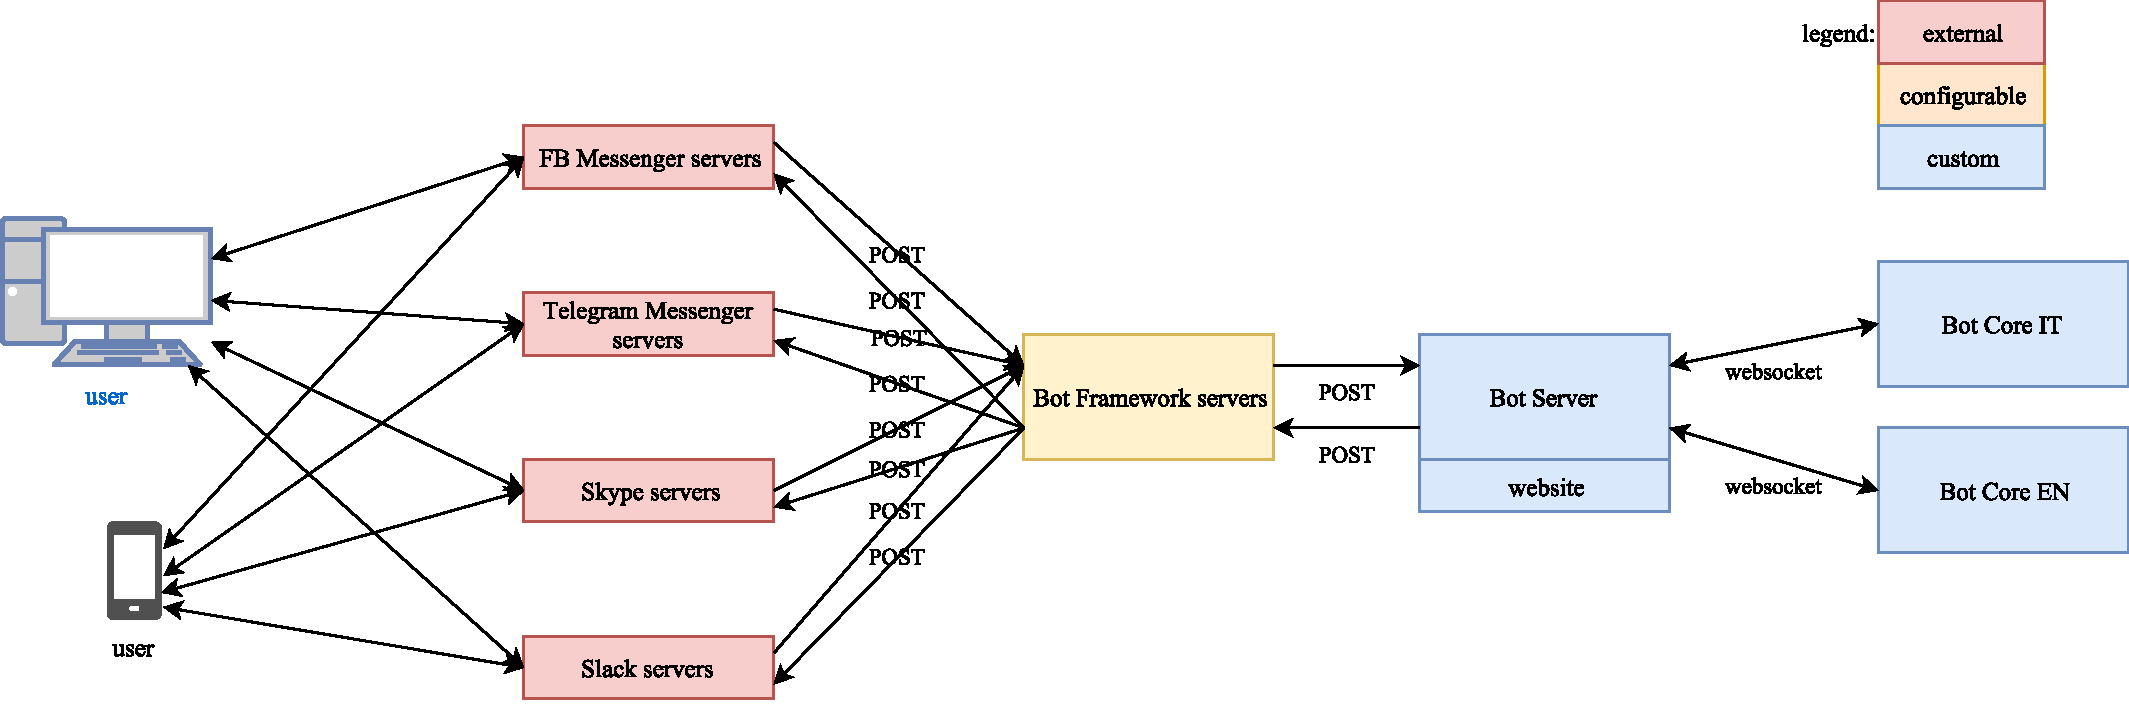
\includegraphics[max width=\linewidth,max height=8cm,keepaspectratio]{figures/physicalComponents}
    \caption{The physical components involved}\label{fig:physicalComponents}
\end{figure}

The communication between the two custom components (in blue in the figure) is done over a websocket to allow asynchronous messages to be sent in both directions, without using polling techniques that may consume resources and bandwidth. The Bot Server exposes two different endpoints for Bot Cores, one for the English version and one for the Italian one. Those endpoints thanks to HTTPS protocol offer a reliable channel that provides data encryption to protect data in motion and authentication through a symmetric key shared between the two parts. The data is transferred between those two components with the JSON standard over the websocket, with a format that does not depend on any specific messaging platform.

The Bot Server is not put directly in contact with the Messaging platforms because it would have required to implement all the webhook endpoints for them and also to translate from and to all the platform dialects. The most easy way to implement it has been found by interacting with a third-party component (Microsoft Bot Framework) that can be configured on a web portal to reach the different platforms. This removed a lot of implementation effort but brought to an architecture that is not very elegant and compact. The communication between the Bot Server and the Bot Framework is done in a way that is similar to the one required by messaging platforms: both components expose web endpoints (that must provide HTTPS connections with digital certificates that have as root a trusted CA) that are used for one-directional communications (the only response that is given is a status code that represent the outcome of the request) and each message is sent independently in its direction.

The supported platforms that have been configured for users to chat with the bot are the following:

\begin{itemize}
	\item Telegram: chosen because it is easy to create bots and is a $``$must$"$  for historical reasons. This channel is available both for English\footnote{\url{https://telegram.me/botcycle\_bot}} and Italian\footnote{\url{https://telegram.me/botcycle\_it\_bot}} languages. A particularity of this platform is that it allows using a special kind of buttons that enables the user to send his current location.

	\item Facebook Messenger: chosen because linked to Facebook it is one of the messaging platform with the biggest number of potential users. This channel too is available both in English\footnote{\url{https://m.me/BotCycleEn}} and Italian\footnote{\url{https://m.me/BotCycleIt}} languages. Similarly to what happens on Telegram, a special button can be built with the capability to pick a location on a map.

	\item Skype: exploiting the exclusive Bot Framework support for the platform, that is not usable otherwise, this channel is added both for English\footnote{\url{https://join.skype.com/bot/2cb007d1-5dd5-441a-8503-23268e2df32d}} and Italian.\footnote{\url{https://join.skype.com/bot/db2aa777-2e46-40fc-9e49-9bc9d1db201b}} However the majority of people do not even know that bots can live on skype.

	\item Slack: used for internal experimental testing on a dedicated workspace.

	\item Web site: a dedicated website\footnote{\url{https://botcycle-server.herokuapp.com/}} allows to test the bot without using messenger apps.
\end{itemize}

The main role of the Bot Server is to receive the messages on one side and provide them to the other one, by transforming their representation. The Bot Framework works well in the direction of receiving the messages from the user, but on the other directions does not provide all the features specific to the messaging platform. For instance, both on Facebook Messenger and on Telegram, buttons can be shown to the user in order to send the current position, while other platforms do not support it. To send these types of messages, it is necessary to send attachments in the native form of the platform ('\textit{quick\_replies}' with \textit{'content\_type': 'location'} for Facebook, \textit{'reply\_markup'} with \textit{'request\_location': true} for Telegram). Furthermore, this component also provides a web page where users can test the bot without using messaging platforms, as has been described previously. Also the Bot Server source code is made available openly,\footnote{\url{https://github.com/MartinoMensio/botcycle-server}} and makes internally usage of the Botkit library\footnote{\url{https://botkit.ai/}} to interface correctly with the Bot Framework.

Having two different custom components has many advantages: both conceptual and practical. The main conceptual advantage is that the coupling with messaging platforms is reduced: the bot core does not know anything related to them, and interacts with a representation of data that is human-readable and has no dependencies. The practical ones are many, generated from different needs, first of all performance. The Bot Server does not require high computation resources because is simply a proxy that manipulates the representation of information. The Bot Core instead, running Neural Networks to classify the sentences, needs disk space and RAM (the language models are quite huge), together with a computing power that should be sufficient to produce outputs in short times. The Bot Server instead requires to host a web server with a fixed hostname and with good certificates provided by a CA trusted from the Bot Framework. This hostname needs to be configured as a webhook endpoint to whom send POST requests with the incoming messages.

Having those needs and opting for a cheap feasible option (without buying a powerful VPS with all those features), the choice has been to split those components. The Bot Server is hosted on heroku\footnote{\url{https://www.heroku.com/}} with a free plan that has limitations in computing power and space, but fits the requirements for this component. Especially, the platform supports natively HTTPS that are covered by a wildcard certificate (every application receives a URL that matching with \textit{$\ast$ .herokuapp.com} is covered). Websites and Web Server applications can easily be created (using one of a large set of supported languages and frameworks) and pushed to the platform and the deployment will occur with no pains in configuration. Having the websocket endpoints exposed on the Bot Server, the Bot Core does not require to act as a server: no hostname is required, no certificate, no port forwarding on NATs, no ports open on the machine that runs it. This enforces a lot the security of the system. Furthermore also the websockets are HTTPS as offered by the Bot Server, so no plaintext interactions can be intercepted.

To make clear how all the components work together, let us follow what happens from when a user sends a message until he receives back a response. First of all, the user connected to a messaging platform (Facebook Messenger) sends some text, that arrives to the Facebook Servers. From there, since the destination account is a page that has been configured to receive messages at a certain webhook location, the message is sent to the Bot Framework. From the Bot Framework, the message is forwarded to the Bot Server that is finally one of the two custom components that has been developed. The Bot Server, checking that a Bot Core is connected over websocket for the specific language, delivers the message. The Bot Core processes the message (NLU, Information Retrieval, Response Generation) and replies on the websocket. The Bot Server transforms the response for the dialect of the destination platform and forwards the message to the Bot Framework that delivers it to the Facebook Servers. Finally the user receives the message.

The flow is quite intricate but has all the advantages listed above.

\section{Natural Language Understanding}
\label{implementationNLU}

This section focuses on the implementation that has been done relatively to the Natural Language Understanding described on the previous chapter \ref{approachNLU}. Firstly, a description is done of the external NLU provider that has been used to initially handle the understanding process and successively has been kept as a single-turn dataset collector and manager (\ref{implementationWit}). Then the discourse will cover some details about the frameworks used for implementing the neural networks in \ref{implementationNN}, and also about some specific issues risen in the development in \ref{implementationNNDetails}. A dedicated subsection is then given to word embeddings in \ref{implementationWV} and the last part explains how the datasets have been collected and preprocessed to uniformly be fed to the neural network in \ref{implementationDatasets}.

\subsection{Wit.ai exploitation}
\label{implementationWit}

In the early stages of the bot, the Natural Language Understanding has been delegated to an external provider: wit.ai.\footnote{\url{https://wit.ai/}} It was chosen for its simplicity to use and for being a standalone product that just provides NLU usable through a web API.

While giving the advantage to have an almost ready to use NLU (the configuration of intents and entities requires few steps and few examples), it also helps building a dataset. All the sentences that are sent for analysis are stored in a inbox, that can be analyzed and the responses can be interactively fixed and validated (inserted in the dataset). The dataset can also be downloaded, and because it is stored in comprehensible JSON format can be used as annotated dataset to later train another NLU system. A limitation of this service is that it handles only single-turn interactions, so the datasets that have been collected for both Italian and English languages can be only used for this type of interaction.

This stage of development has been done in order to understand the main needs of the users, and progressively new intents and examples have been added. On the other side, this experimentation also helped understanding what the NLU tasks are, giving an orientation in the very big landscape of Natural Language Processing. This helped directioning the study of literature towards approaches that could do a similar sentence classification and parameters extraction. During this stage, it has been noticed that for the intent classification task a promising approach is to use Recurrent Neural Networks, so the studies (both theoretical and practical) went deeper in exploring this field.

\subsection{Neural Networks frameworks}
\label{implementationNN}

As of today many open source libraries and frameworks are available for NLP tasks, using different programming languages and different approaches. The most important ones are:

\begin{itemize}
	\item Stanford Core NLP:\footnote{\url{https://nlp.stanford.edu/software/}} a java library that provides Tokenizer, NER, POS, Dependency Parsing, Coreference Resolution for languages: English, Arabic, Chinese, French, German, and Spanish;

	\item NLTK:\footnote{\url{https://www.nltk.org/}} a python library that focuses on Tokenizers, n-grams, POS, NER;

	\item Syntaxnet:\footnote{\url{https://github.com/tensorflow/models/tree/master/research/syntaxnet}} a neural-network NLP framework for TensorFlow. Helps building POS and Parsers. It contains pre-built models for POS and parsing. It is the most accurate parser for english, able to parse correctly garden-paths;

	\item SpaCy:\footnote{\url{https://spacy.io/}} an open source NLP framework that provides Tokenizer, NER, POS, Dependencies, Word Vectors, Parsing for different languages with the goal of being ready to use with pre-built models, and also fast.
\end{itemize}

But from what has been explored, those libraries focus on a selected subset of NLP tasks, and we wanted to implement Neural Networks to have full control of the process.

Experimenting with Neural Networks has become easier and easier in the last years thanks to open source libraries that provide high-level APIs and, being used more and more, the support is really easy to obtain on online communities (such as StackOverflow\footnote{\url{https://stackoverflow.com/}}) or on the official documentation or directly on the official code repositories (by means of interlined comments or $``$\textit{self-documenting code}$"$~\cite{raskin2005comments}). The programming languages that are supported for Neural Networks are many, but the most used nowadays is Python. In Python the most used frameworks are Keras\footnote{\url{https://keras.io/}} and TensorFlow.\footnote{\url{https://www.tensorflow.org/}}

For choosing between Keras and Tensorflow, experiments have been done with both. It is important to say that the two frameworks are not uncorrelated, because Keras as default backend uses TensorFlow and TensorFlow recognizes Keras as its high-level interface.\footnote{\url{http://www.fast.ai/2017/01/03/keras/}} So the problem is simply to choose the abstraction level desired.

Initially, when trying to emulate a RNN approach for Intent Classification (see section \ref{soaIntent}, Keras has been used to implement it. Without considering the data preprocessing part that is needed to get the desired shape and values for the inputs and outputs (as inputs word vectors corresponding to the words in the sentence and as outputs the corresponding intent type), the building of the computation graph (a bidirectional LSTM layer followed by a densely connected layer) and its training just required few lines of code.

But when trying to implement less regular models, such as the encoder-decoder of~\cite{liu2016attention}, the criticality of using only high level API came out, especially considering complex parts like output dependencies.

For this reason a comparison has been done in order to choose what implementation path to follow. Table~\ref{tab:kerasVsTf} summarizes the main differences found between Keras and TensorFlow.

% !TEX encoding = utf8
% !TEX root = ../main.tex

\begin{table}
  \begin{tabularx}{\textwidth}{XXX}
    \toprule
    \textbf{feature} & \textbf{Keras} & \textbf{Tensorflow} \\
    \midrule
    Abstraction level & High & Can go down to reach single operations, but also high level API is provided by lots of classes \\
    \midrule
    Learning difficulty & Quite easy & More difficult, lots of details to consider \\
    \midrule
    Support for complex operations & Focuses more on simple regular layers and cells & Lot of already defined classes, and also helpers function that can help building complex operations \\
    \midrule
    Best for & Rapid prototyping & Advanced operations \\
    \midrule
    Documentation & Documentation good for what is implemented & Documentation gap between trivial and advanced \\
    \bottomrule
  \end{tabularx}
  \caption{A comparison between Keras and TensorFlow}\label{tab:kerasVsTf}
\end{table}

Let us see in more details what is the support provided by both libraries for building recurrent neural networks in the following paragraphs.

\subsubsection{Keras Recurrent API}
Similarly to what happens with feedforward neural network, also when working on recurrent ones handling Keras layers is like playing with LEGO:\footnote{\url{https://www.lego.com/}} blocks can be easily stacked one on the top of the other (also forks and joins are quite easy to perform). Keras Recurrent API is described extensively on its documentation,\footnote{\url{https://keras.io/layers/recurrent/}} while here only a quick overview is performed.

To define a recurrent layer in Keras the class \textit{keras.layer.RNN} takes as argument a RNN cell. Some parameters can be used to define how the layer will behave. A RNN cell is a class that has a call method that takes as input the actual input and the current state and produces the output and the next state. Different implemented cells exist.

\begin{itemize}
	\item \textit{SimpleRNNCell}: a cell that simply concatenates the input with the previous state and passes it through a feedforward layer;

	\item \textit{GRUCell}: Gated Recurrent Unit~\cite{cho2014learning};

	\item \textit{LSTMCell}: Long-Short Term Memory layer~\cite{hochreiter1997long}.
\end{itemize}

Layers can be easily stacked and the creation of deep recurrent network is very easy. Networks that are a simple stack of different layers (Recurrent, Dropout regularizations, Dense feedforward) will not find any problem in implementation. But when the networks are not so linear in the flow or when some advanced layers are required, there might not be an already implemented solution. For example there is no native implementation for \textit{seq2seq} models and layers, no \textit{Attention} mechanism and it is not possible to have a ready to use help for doing output dependency modeling (feeding back the outputs in a decoding layer). They can be implemented with the existing API, but they are not part of the library itself (some implementations can be found online,\footnote{\url{https://github.com/farizrahman4u/recurrentshop}} but the number of people working on it is order of magnitude smaller than the one involved in the TensorFlow community).

\subsubsection{Tensorflow Recurrent API}
Also tensorflow has classes for defining RNN layers and RNN cells. But there is more:

\begin{itemize}
	\item More cells: instead of a single implementation of LSTM and GRU, a wide variety of cells can be chosen

	\item More wrappers: wrappers can be used to encapsulate cells. DropoutWrapper, AttentionWrapper and a lot more can be added to the cells

	\item Seq2Seq native support: classes for defining encoders and decoders, with some helpers for modeling output dependencies can make a lot easier to build complex models that are not a linear chain of layers but contain links that move backwards in the stacked layers (as in output dependencies, where the output label is fed back to the decoder RNN). For example to build a decoder that considers output dependencies, in tensorflow three components are needed: a RNN cell (e.g. LSTMCell), a CustomHelper (that is responsible to provide values to the cell and take the outputs by simply declaring three custom functions) and a BasicDecoder that combines the cell with the helper and builds a layer. By dividing the roles of the cell and of the helper, a complex decoder can be built without a big effort.
\end{itemize}

More details about the available classes can be found in the official documentation of the seq2seq package.\footnote{\url{https://www.tensorflow.org/api\_docs/python/tf/contrib/seq2seq}}

\subsubsection{Decision}
The objectives of the decision between the frameworks are:

\begin{itemize}
	\item Ability to build the proposed network without too much headache. Especially for the decoding stage, some advanced wiring is needed and would like not to start from scratch (being really error-prone) but have some native support from the library;

	\item Code readability and maintainability: possibly using quite high level operations, no reinventing the wheel (in a buggy version)

	\item Quite good performances
\end{itemize}

Considering these objectives, the choice has been to use the native TensorFlow APIs for building the solution, using the seq2seq package for faster implementation. The additional work required to build even simple networks is compensated by the great flexibility of the library.

\subsection{Graph details}
\label{implementationNNDetails}

Implementing a neural network with tensorflow needs understanding some basic concepts.

First of all, the difference between defining a computational graph and actually doing operations. This is the concept of \textit{tensors}: they are a generalization of (multidimensional) vectors that will be used to contain values. Using and connecting them in computational graphs means defining how the values contained will be processed. The big difference with normal variables is the time of execution of the computations defined.

If in a programming language we have two variables  \( a=3,b=1 \)  and we sum them, when the instruction of sum is executed  \( c=a+b \)  the resulting variable will contain the result  \( c=4 \) . Instead defining a sum between tensors  \( a=tf.Variable \left( 3 \right) ,b=tf.Variable \left( 1 \right)  \) , when the instruction of  \( c=a+b \)  is executed the resulting tensor will not contain  \( 4 \) . It will be stored that c can be computed by summing what is contained in  \( a \)  and  \( b \) . In this way the operations can be defined once and the same computational graph can be run different times. To actually run the graph it is necessary to build a session, that is the execution environment. But in order to have different inputs to the same graph, there is the need to define the starting tensors not as Variables but as placeholders. Later when running the session, the placeholder values can be fed to the graph and the results can be evaluated. The library is powerful in how allows to define variables that can be initialized and automatically optimized by internally using the packpropagation of gradients. The only things that the programmer needs to do is to define the graph with all the tunable variables and declare a loss function to be optimized. No manual calculation of gradients, it is handled by TensorFlow.

The most difficult things to do while using this library are: \textit{i)} know which operation to use, because there are so many classes available that only after a deep dive into documentation a solution is found; \textit{ii)} manipulate in the correct way multi-dimensional tensors, without making confusion. Both difficulties decrease by the increasing time used to experiment with it, but it is important to understand soon how to work with the $``$\textit{axes}$"$  parameter, crucial to perform reduction operation over the correct dimensions in nearly all the operations.

As has been discussed in the approach part, the chosen graph to be used in single-turn interactions is the encoder-decoder joint approach of~\cite{liu2016attention}. The paper comes with a TensorFlow implementation that is not complete:\footnote{\url{https://github.com/HadoopIt/rnn-nlu}} output label dependencies are not considered. Another negative property of the implementation is that it does not use a recent API, that would provide higher level functionalities and helper functions. Another implementation has been found that uses a more recent API and is really a lot more understandable that the original one.\footnote{\url{https://github.com/applenob/RNN-for-Joint-NLU}} It makes use of the \textit{seq2seq} native package,\footnote{\url{https://www.tensorflow.org/api\_guides/python/contrib.seq2seq}} that can be used for all the quite complicated networks that process sequences, like NMT or generative processing by employing classes that are relatively simple to use with respect to what they do.

So this last implementation has been used as starting point. Starting from this last implementation, that highly depend on the ATIS dataset~\cite{hemphill1990atis} in the preprocessing part, a slightly different implementation has been developed. The differences are described in the following paragraphs.

\subsubsection{The differences}
The main changes are not on the network structure, that is the one of the original paper, but in some details about the inputs and outputs.

First of all, the inputs of the computational graph, previously feeded as word indexes, have been changed to string tensors (that exist as native type in TensorFlow although its math-preponderance). In this way the dictionaries are part of the graph. Translation from word to indexes and the inverse operation is possible thanks to the package \textit{tf.contrib.lookup} that can be used to implement lookup tables for both the directions (words to indexes and indexes to words).

Then, having the lookup operations inside the computational graph and having the string tensors as inputs, it has been possible to define different ways to obtain the embedding values with the same interface. Both proceeding implementations contained the embedding matrix as a trainable Variable with size  \(  \left[ vocabulary \_ size  \times  embedding \_ size \right]  \) , and this embedding technique has been moved in a specific class. The other way to obtain the embedding values, that corresponds to pretrained fixed values, is to use an external library (SpaCy, see the details and implications below in word embeddings section \ref{implementationWV}) to get those values. The library requires words as parameters to get their representation, and it would not have possible to pass the word ids as in the previous implementation.

Having another class that wraps the external library call to get the embedding vectors, it is possible to test the two different approaches (trainable embeddings versus fixed pretrained embeddings) and some measures have been done showing a boost given by the second approach empowered by big corpora.

To make more understandable also the management of output dictionaries (intent types and IOB annotation types), the same strategy has been used. This time only trainable embeddings not precomputed have been used, because the words do not belong to the English or Italian dictionary (for example the word \textit{search\_bike} or \textit{B-location}).

The last kind of modifications that have been done are relative to saving the models trained and being able to resume them for inference time. This is possible thanks to the naming of tensors, that allows to save the computational graph and the values of the variables to the disk and resume it without re-defining all the variables that were present previously. To interact with the graph, it is possible to retrieve the input and output tensors by name and all the intermediate steps will be internally managed by TensorFlow. As will be described in \ref{implementationSpacyPyFunc}, the only parts that cannot be serialized are the external python functions, but a solution exists also for this problem.

\subsubsection{Multi-turn}
Relatively to the multi-turn implementation described in subsection \ref{approachMultiTurn}, the modifications for considering the previous agent turn are only on the preprocessing step, while for doing the top level intent RNN an addition has been done on the top of the intent logits. As can be seen in Figure~\ref{fig:approachMultiTurnDifferences}, instead of passing them to a softmax layer that estimates their value, the current turn intent logits are passed to a LSTM cell that receives as previous state the previous intent value. This specific point has been critical because the original idea was to propagate the previous state directly, as a vector of floating values, that would have allowed the backpropagation to go through the previous turns and optimize also tunable parameters of the past. But maintaining the state of this cell would have been difficult in the training phase specially. The training samples would have needed to be fed in the correct order (using the cell in stateful mode), or the whole discussion would have needed to be fed for each new user sentence. Both of these solution are not good for performance, so the decision has been to use directly the previous value of the intent instead of the state of the cell. This is something that is also done in sequence to sequence approaches, where previously generated words are fed as inputs to the decoding stages. In this case, the previous value of the intent is translated from string to an index (using the lookup table) and then transformed into a one hot encoding (a vector of zeros with a  \( 1 \) at the correct index).

\begin{figure}[!htbp]
    \centering
    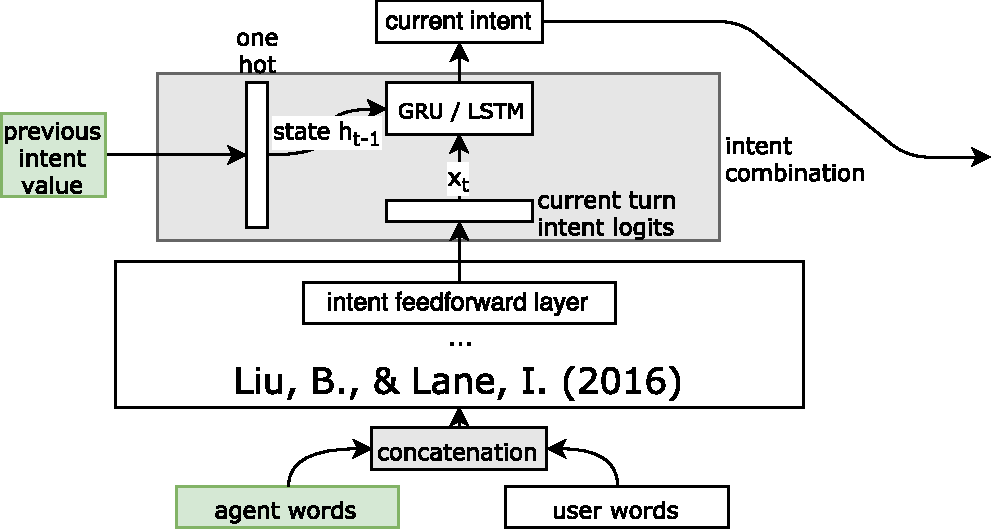
\includegraphics[max width=\linewidth,max height=8cm,keepaspectratio]{figures/approachMultiTurnDifferences}
    \caption{The differences of the multi-turn with respect to~\cite{liu2016attention}}\label{fig:approachMultiTurnDifferences}
\end{figure}

\subsection{Word embeddings}
\label{implementationWV}

To work with word embeddings different strategies and libraries can be applied. The most TensorFlow-purist one is to declare the embedding matrix (one vector for each word) directly as a TensorFlow variable. This is the simplest solution from word embeddings that are randomly initialized and are tunable. However it may have implementation and memory issues when the values come precomputed on bigger corpora (all the embedding matrix is loaded simultaneously in memory, and it is very important to keep only one copy of it in memory\footnote{\url{https://stackoverflow.com/questions/35687678/using-a-pre-trained-word-embedding-word2vec-or-glove-in-tensorflow}}). Furthermore, it is necessary to get the word embeddings from third party sources and manage the download of them carefully (the implementation presented in this work is based on docker containers\footnote{\url{https://www.docker.com/}} to provide high portability). And third party libraries can be necessary also to do common text processing or IOB label management.

For all these reasons, our implementation integrates a neural network library with a NLP library. For NLP, Spacy has been chosen for its good performances\footnote{\url{https://spacy.io/usage/facts-figures}} and models supporting word embeddings.\footnote{\url{https://spacy.io/models/}} It has been used also in an early stage of experimentation for identifying the entities with its native functionalities. The natively provided models come in different sizes, where the most spatial occupation is given by the word vectors. For example on the English language, four different models are available\footnote{\url{https://spacy.io/models/en}} where also the biggest one only occupies around 600MB.

For some other non-english languages only the smallest model is available, that does not contain precomputed word vectors. Instead, using character-based information, SpaCy provides contextual tensors\footnote{ https://spacy.io/usage/vectors-similarity$\#$ in-context  } that are estimated by applying a 4-level convolutional network sensitive to up to four words on either side of a word. The performances of these tensors are also analyzed in the validation chapter \ref{validationMeasures}, but generally they are not as good as word vectors precomputed on large corpora. However SpaCy allows quite easily to build new models that can integrate a native language model with externally computed word vectors.

\subsubsection{The tokenization of spaCy}
For splitting the sentences into words, with knowledge of the common problems explored in section \ref{soaVocabulary} when discussing about keeping or removing punctuation and special cases like apostrophes, the chosen approach is the one employed by the library SpaCy. This is done by applying rules specific to each language. Just as an example, punctuation is split off, like commas or periods at end of sentences, but "\textit{U.K.}" remains one token. English expressions like $``$\textit{don't}$"$  are tokenized into [$``$\textit{do}$"$ , $``$\textit{n't}$"$ ] and for this reason a lot of rules are applied. For other languages that do not have a full model, like the Italian one, the tokenization is more trivial because no one has yet worked on those rules. However it is always done better than a whitespace tokenization (splitting the words basing on spaces or other separator signs) combined with punctuation removal.

\subsubsection{Integrating SpaCy with TensorFlow}
\label{implementationSpacyPyFunc}

To integrate the Spacy NLP utilities inside a computation graph defined in TensorFlow, two different things have been done.

The first one is relative to the tokenization. To simplify the process of transform the sentences into vectors of words, it has been chosen to put this operation in the preprocessing step. A motivation for this solution is that the ATIS dataset~\cite{hemphill1990atis} has a predefined word tokenization based on whitespaces. To maintain the measurements comparable with other papers, in this specific case the tokenization is not modified while for other corpora, that only define sentences without saying how the words are separated, the SpaCy tokenization is applied. Having different tokenization models, to simplify the feeding of inputs the tokenization has been managed in the normalization procedure of datasets. The source datasets are preprocessed and saved to disk in a uniformed format (that can be seen in the \textit{preprocessed} folders\footnote{\url{https://github.com/D2KLab/botcycle/tree/master/nlu/data}}).

The second point of contact between the NLP library and the computational graph is established when the word embedding values are retrieved. Being inside the computational graph the only way to call a custom function, as a block that works with tensors, is to use the \textit{py\_func} helper. This method allows to put in the graph a python function, possibly idempotent to avoid side-effects that may generate unwanted behaviour since the training is usually done together with randomization of samples, that will receive and produce numpy arrays\footnote{\url{https://docs.scipy.org/doc/numpy-1.13.0/reference/generated/numpy.array.html}} translated back and forth to tensors for the graph.

The only problem of using this helper is that the graph will not be fully serialized to disk for future usage. The solution to this problem is to declare again the same function when the restoration of the graph and parameters are done, before declaring and using a running session.

\subsubsection{Italian word embeddings}
As has been said previously, for the Italian language, SpaCy has an incomplete model that does not contain precomputed word vectors but only contextual tensors (generated on the fly by a convolutional network) are available. For this reason, a side work has been done, taking the Wikipedia Italian corpus\footnote{\url{http://dumps.wikimedia.org/itwiki}} and computing GloVe vectors on it. Some preprocessing has been done to extract the text only of the dump with a mix of tools written by the SpaCy developers\footnote{\url{https://github.com/explosion/spacy-dev-resources}} and people from the University of Pisa.\footnote{\url{http://medialab.di.unipi.it/wiki/Wikipedia\_Extractor}} From the text, cleaned of all the markup and XML tags, a re-tokenization is applied to feed correctly the text to the GloVe algorithm.\footnote{\url{https://github.com/stanfordnlp/GloVe}} In this way both the dictionary and the tokenization used in the training of the word embeddings is the same that is used by the computational graph.

The output of this process is a SpaCy model that is made available openly\footnote{\url{https://github.com/MartinoMensio/it\_vectors\_wiki\_spacy}} and can be installed easily with \textit{pip}.\footnote{\url{https://pip.pypa.io/en/stable/}}

\subsection{Datasets collection}
\label{implementationDatasets}

This last subsection contains some details about how some datasets have been collected for the specific bike sharing domain. The goal is to be able to have enough annotated sentences for both single and multi-turn, in order to train the selected approach and be able to provide measures (see next chapter \ref{validationNLU}) that have a bit of statistical significance.

Starting with the single-turn settings, it has been described in subsection \ref{implementationWit} that wit.ai has been exploited to gradually collect sentences. By using this online platform it has been quite simple to annotate new samples, that also come from online usage of the bot thanks to the recording capabilities. The platform offers support for a quite wide variety of languages, and the English and Italian are between them.

Instead for the collection of multi-turn dialogue sessions, a logging of all the incoming and outcoming messages has been done in the local database to capture as more dialogues as possible. With the basis of these dialogues, that are characterized by some features typical of a very restricted experimental setup (such as repetitivity and lack of variety, high ratio of wrong responses, preponderance of sentences sent to test the bot and not to really use the information provided), a successive cleaning has been done to only insert proper sentences in the training set. This cleaning has been done to identify the relevant dialogues that should contain multi-turn interactions, using a TSV format that allows an easy modification of values without requiring any special environment.

But a big problem avoided collecting a good dataset: a circular dependency. The system was expected to collect a dataset for the multi-turn dialogues while it only provided single-turn capabilities. The most common example is when the user does not provide a required parameter (e.g. searches a bike without saying where), the bot asks for the location, the user provides it without forming a complete sentence (only the entity value provided, without the $``$\textit{i am in}$"$  prologue) and the bot fails because no intent has been detected (lack of the multi-turn model). To solve this problem other strategies may be applied, like building a restricted dataset by hand without an online setting, and proceeding with incremental cycles of testing, collecting and training. Or even better would be to enable a Reinforcement Learning based approach to increase the performance while conversing with the user.

% !TEX encoding = utf8
% !TEX root = ../main.tex

\chapter{Validation}
\label{validation}

This chapter is relative to the validation of the dialogue system. What is evaluated can be divided into two main parts: one is relative to the NLU approach described in the Chapter~\ref{approach} (Subsection~\ref{approachNLU}) considering different datasets and different variations of the model; the second one instead focuses more on the bot prototype, looking at some measures that can be done to evaluate its global performance from the point of view of the users.

\section{NLU evaluation}
\label{validationNLU}

This section  describes the datasets used (Subsection~\ref{validationDatasets}), the evaluation protocol and the measures analysis (Subsection~\ref{validationMeasures}).

\subsection{Datasets}
\label{validationDatasets}

In the search of datasets available for the Natural Language Understanding, two main types of corpora have been found, respectively for single-turn and for multi-turn interactions. Here we provide a list of them, with some statistics and details of each one. About the language of the datasets, the found ones are in English both for single: no availability of Italian annotated datasets have been found. The Italian dataset used for the embeddings is discussed in the last part of this subsection, but the key point is that these corpora are not annotated because the word embeddings algorithms are unsupervised. For both single and multi-turn, in addition to the available datasets, an English and Italian dataset is proposed for the domain of bike sharing, collected with the methods described in the previous Subsection~\ref{implementationDatasets}.

\subsubsection{Single-turn}
For the single-turn, a lot of datasets can be found online, each one with a different domain of application. The characteristics of these datasets is that each sentence is annotated with the values of the intent (a feature of the whole sentence) and of the slots (word groups, also called \textit{spans}). While the annotation of the intent is more or less standardized, for the annotation of slots different notations can be used, representing different features. Those specific elements will be explained for each dataset.

\paragraph{ATIS}
The first dataset, used historically for the tasks of intent detection and slot filling, is Air Travel Information System (ATIS)~\cite{hemphill1990atis}. This dataset contains transcriptions of questions obtained from the Official Airline Guide\footnote{\url{https://www.oag.com/}} in 1990: each question is annotated with its intent, over 18 different intent types, and with the relative slots, over 127 \texttt{IOB} slot types (corresponding to 80 slot types reducing the \texttt{B-} and \texttt{I-}). The slot types correspond to entity types with a specific role: for example the slot type \texttt{fromloc.city\_name}  corresponds to the entity type \texttt{city\_name} with the role \texttt{fromloc} that expresses that this is the source city in the sentence. The dataset notation is done using the \texttt{IOB} format. For this reason, the inputs and outputs of the dataset are provided already tokenized by using a whitespace tokenizer. This is the only dataset considered that constraints the division of words because the other ones usually represent slots as start and end indexes of the sentence.

The dataset has 4978 training samples and 893 test samples: the original division is only in two splits, no ``development'' set is available. However some works have additionally divided the training set into two parts to leave the validation set on its own for the final evaluation and not for the hyperparameters optimization.

\paragraph{NLU Benchmark}
Another dataset that has been used in the specificity of single-turn interactions is the \textit{nlu-benchmark} that is published by Snips\footnote{\url{https://snips.ai/content/sdk-benchmark-visualisation/}} as an effort to compare and evaluate different NLU commercial providers like Amazon Alexa,\footnote{\url{https://developer.amazon.com/alexa}} Google Api.ai,\footnote{\url{https://api.ai/}} Microsoft Luis,\footnote{\url{https://www.luis.ai/}} Apple SiriKit,\footnote{\url{https://developer.apple.com/sirikit/}} IBM Watson Conversation,\footnote{\url{https://www.ibm.com/watson/developercloud/nl-classifier.html}} Facebook Wit,\footnote{\url{https://wit.ai/}} and Snips\footnote{\url{https://snips.ai/}} itself. The dataset used for their benchmark\footnote{\url{https://github.com/snipsco/nlu-benchmark}} is considered here for the custom intents: 7 different intents are provided over a total of 1942 training samples and 100 test ones. Instead the entities are annotated on spans directly, because the sentences are provided pre-split on the edges of the slot values (e.g. [``\textit{Add another }'', ``\textit{song}'', ``\textit{ to the }'', ``\textit{Cita Romántica}'', ``\textit{ playlist. }''] where ``\textit{song}'' and ``\textit{Cita Romántica}'' are two different slots). There are 39 different slot types.

This dataset has been used by Snips to do a benchmark that considers only the intents, but on the measurements we show also the results for the slots.

\paragraph{Wit.ai}
More specific to the prototype built for this project, BotCycle, two single-turn datasets have been collected with the support of wit.ai platform: one in English and one in Italian. The collection of samples begun with the early stages of the prototype, which was relying on \textit{wit.ai} for the understanding part back then. This platform provides a friendly GUI where the intents and slots can be configured, and also some training samples can be provided. Moreover it keeps track of the ``inbox'' messages used in operational environment, that can be later reviewed and added to the gold standard. Even when the understanding part switched to local deployment, we kept sending the requests for processing to \textit{wit.ai} in order to continue increasing the dataset. With this technique we collected 522 samples for the English language and 95 samples for the Italian one.

As described in subsection \ref{approachTypes}, there are 11 intents types and three slot types belonging to the same type of entity: \texttt{from.location}, \texttt{to.location} and \texttt{location} without a specific role. The slots are annotated by providing the start and end indexes, together with the intent type and the optional role.

\subsubsection{Multi-turn}
Instead for the multi-turn NLU, wich is described in subsection \ref{approachMultiTurn}, the number of datasets used is more restricted because less have been found with the required characteristics. The data that we wanted had to contain multi-turn sessions with messages from both sides, where at least on the user sentences it could be possible to obtain the intent value and the slot annotations.

The problem of multi-turn has been analyzed mostly on proprietary datasets~\cite{shi2015contextual,xu2014contextual,bhargava2013easy}, or requiring a participation in a challenge (like the Dialogue State Tracking Challenge~\cite{williams2013dialog}). Others, focusing mainly on memory networks and simple questions, are not very relevant for the multi-turn goal-oriented problem (bAbI\footnote{\url{https://research.fb.com/downloads/babi/}}). The Frames dataset~\cite{asri2017frames} is publicly available but it only contains a single intent (\texttt{book}), and focuses more on the tracking of user and machine actions.

\paragraph{Key-Value Retrieval}
The only dataset found in literature is the Key-Value Retrieval (KVRET)~\cite{eric2017key}, that contains sessions of interaction between a driver and his smart car. Each session begins with an utterance of the driver that clearly states his intent (out of 3 possible values: Calendar Scheduling, Weather Information Retrieval, POI Navigation), and the subsequent turns of both parties continue the dialogue to refine the search and to reach the desired final response. About the annotation of the slots, they are available but not annotated in a straightforward way: each slot (15 types available) is stored with its value, but there are some problems in identifying their displacement in the sentences, because a normalization step would have been required. The major problems are:

\begin{itemize}
	\item trailing spaces in the slot annotation: solved by trimming strings;
	\item capitalization differences between slot annotation and text of the sentence: solved by applying match insensitive;
	\item slots annotated on later turns referring to previous turns: solved by reversing the look-up processing order on the sentences and annotations, in order to enable backward references to text;
	\item multiple matches for the same word in a sentence: by keeping the forward slots to be referenced, sometimes multiple entities overlap partially in the sentences, that is not allowed by the \texttt{IOB} annotation scheme;
	\item incomplete slot value: for example ``\textit{take my pills}'' in the sentence is annotated as ``\textit{take pills}'', and this is not solvable by simple look-up strategies;
	\item entity\ resolution problems:  for example the reference ``there'' is annotated with its resolution (the place mentioned before), or ``\textit{today}'' in the text is annotated as ``wednesday'' in the slots;
	\item other entity resolution problems that could be solved by looking at the attached Knowledge Base: those are not resolved since it is not the only limitation.
\end{itemize}

The selected multi-turn approach, while providing also outputs for the slot labels being trained jointly, is here analyzed mainly under the point of view of the intents, so this is actually not a problem. The main goal is to be able to automatically recognize when a certain session ends or continue, where a time-based session split can be misleading and a working solution should rely on the contents only.

This dataset, therefore, satisfies our needs: each sentence is annotated with its speaker and the intent values are available. The preprocessing is composed of three steps: \textit{i)} annotation of the intent from session-level to sentence-level by copying the values; \textit{ii)} concatenation of all sentences, removing the concept of session that remains only on the intent values; \textit{iii)} consider as samples only the driver sentences, each one stored together with the current and previous intent value and with the previous sentence of the agent.

With this setup of the samples, on the training set there are  $1583$ intent changes over $6429$ samples, while on the test set $189$ changes over $820$ samples.

\paragraph{BotCycle multi-turn}
As for the single-turn, a targeted dataset is needed for the specific application to the bike sharing domain. For this reason, all the conversations between the user and the bot have been recorded, and from them some sessions have been cleaned up, eventually correcting the predicted outputs. The conversations have been generated from a restricted team of testers that knew the limitations of the system and focused the interaction on the actual types of things the system is able to do. Through this technique it has been possible to collect $73$ sessions with an average length of $12.7$ for the English language and $10$ sessions with an average length of $29.4$ for the Italian one (considering sentences from both interlocutors).

Actually, this dataset is nearly unusable for all the limitations that have been noticed in Subsection~\ref{implementationDatasets}, as can be seen also from the quite poor size of the Italian dataset.

\subsubsection{Italian Word Embeddings}
For the Italian Word embeddings actually the datasets available are mainly two: Wikipedia or CommonCrawl. Both can provide statistical information of word co-occurrences and be used to train unsupervised representations like word embeddings.

The Wikipedia Italian dump\footnote{\url{http://dumps.wikimedia.org/itwiki}} consists of nearly 2.3GB of text contained in the articles. This dataset contain quite formal language and does not cover well the entire Italian dictionary (covering only $758358$ different words), but it is the only feasible to be used for such huge calculation.

With proper machines (calculation power and storage), another dataset is the CommonCrawl one, available on a preprocessed version where duplicated sentences have been removed\footnote{\url{http://data.statmt.org/ngrams/deduped/}} to have only a size of 76GB. This corpus contains text found on a lot of websites, and will therefore have a larger dictionary. However, for its size it is impossible to be processed in an environment without server farms.

\subsection{Evaluation Protocol and results}
\label{validationMeasures}

The following paragraphs illustrate the results obtained. First of all, a dedicated evaluation to the Italian embeddings computed will show how the different preprocessing allows to reach higher scores on the analogy test~\cite{mikolov2013linguistic}. Then different variations (such as the embedding dictionary size, the choice of LSTM vs GRU and the usage of attention mechanism) will be measured on the single-turn setting. At the end also some evaluation on the multi-turn setting are shown. To evaluate the performance of the computational graph, a search of commonly used measures has been done. For the ATIS dataset usually~\cite{tur2010left} the performance is evaluated by computing the intent error rate and the F1 measure for the slot filling. It is important to notice that in classification tasks for which every test case is guaranteed to be assigned to exactly one class, F-measure on micro level (globally counting true positives,false negatives, false positives) is equivalent to accuracy. So for both single and multi-turn settings the measure chosen to evaluate the results is the F1 score on the intents and slots (a slot is correctly detected if both type and start and end are correct).

\subsubsection{Italian embeddings analogy evaluation}
To evaluate the goodness of word embeddings, a commonly used test is the analogy test~\cite{mikolov2013linguistic}. Since in the embeddings space, words should distribute relatively to their meaning, semantic relations can be characterized by a translation. For example the relation singular-plural can be exploited to find a plural of one word by using the analogy of coordinates between another pair of singular and plural words (e.g. \textit{queens} = \textit{queen} - \textit{king} + \textit{kings}). The evaluation is done by comparing the predicted word against the true one. Here we are considering the translated version of this analogy test, used by~\cite{berardi2015word} too.

% !TEX encoding = utf8
% !TEX root = ../main.tex

\begin{table}
  \begin{tabularx}{\textwidth}{Xc}
    \toprule
    \textbf{Word embeddings}& \textbf{Accuracy} \\
    \midrule
    Italian values from~\cite{berardi2015word} on Wikipedia & 44.81\% \\
    Computed Italian values on Wikipedia & 58.14\% \\
    \bottomrule
  \end{tabularx}
  \caption{A comparison of the analogy scores for the Italian Wikipedia datasets}\label{tab:italianEmbeddingsAnalogy}
\end{table}

Table~\ref{tab:italianEmbeddingsAnalogy} shows how the different preprocessing, applying the SpaCy tokenization, allows to reach better values for the analogy test.

\subsubsection{Single-turn variations}
For the evaluation of the single-turn approach, since it has been shown to reach State-of-the-Art condition on the tasks of intent classification and slot filling, we are here analyzing how some variations in the structure or in the inputs affect the performances on the collected datasets. The measures shown are the selection of the best score reached over a maximum of 20 training epochs.

The first comparison we want to do is how the choice of embeddings influences the quality of results in terms of F1 score. For this reason in Tables~\ref{tab:intentsEmbeddingsChoice} and~\ref{tab:slotsEmbeddingsChoice} different embeddings strategies are applied (random, contextual tensors, precomputed\footnote{\url{https://spacy.io/models/en}}).

% !TEX encoding = utf8
% !TEX root = ../main.tex

\begin{table}
	\begin{tabularx}{\textwidth}{Lcccc}
		\toprule
		\textbf{Embeddings type} & \textbf{ATIS} & \textbf{nlu-benchmark} & \textbf{wit\_en} & \textbf{wit\_it} \\
		\midrule
		Trainable, randomly initialized & 0.9740 & 0.9928 & 0.9428 & 0.8947 \\
		\midrule
		Contextual tensors & 0.7140 & 0.2542 & 0.4000 & 0.4736 \\
		\midrule
		Medium & \textbf{0.9660} & \textbf{0.9928} &\textbf{0.9714} & 0.8421 \\
		\midrule
		Large & \textbf{0.9860} & \textbf{0.9928} & \textbf{0.9714} & \textbf{0.8947} \\
		\bottomrule
	\end{tabularx}
	\caption{The F1 scores for intent classification with different embeddings}\label{tab:intentsEmbeddingsChoice}
\end{table}

% !TEX encoding = utf8
% !TEX root = ../main.tex

\begin{table}
  \begin{tabularx}{\textwidth}{Lcccc}
    \toprule
    \textbf{Embeddings type} & \textbf{ATIS} & \textbf{nlu-benchmark} & \textbf{wit\_en} & \textbf{wit\_it} \\
    \midrule
    Trainable, randomly initialized & 0.9425 & \textbf{0.9177} & 0.9000 & 0.5000 \\
    \midrule
    Contextual tensors & 0.1658 & 0.0032 & 0.3391 & 0.1818 \\
    \midrule
    Medium (English: 685k keys with 20k unique vectors, Italian~\cite{berardi2015word}: 730k unique vectors) & 0.9588 & 0.8970 & 0.9375 & 0.5666 \\
    \midrule
    Large (English: 685k keys with 685k unique vectors, Italian: 758k unique vectors proposed) & \textbf{0.9649} & 0.9170 & \textbf{0.9689} & \textbf{0.6153} \\
    \bottomrule
  \end{tabularx}
  \caption{The F1 scores for slot tagging with different embeddings}\label{tab:slotsEmbeddingsChoice}
\end{table}

As we can see, the correct choice of word embeddings can play a big difference. The best performance is reached by using fixed pretrained vectors computed on large corpora (with just one exception for the slots on the nlu-benchmark dataset). The contextual tensors provided by SpaCy show a very poor performance, because they are observing only the current sentence and have no knowledge about the real meaning of words. The large model only provides a delta from the medium one on the slot tagging task, while for the intents they have the same performance. For the Italian embeddings, the ``medium'' row corresponds to the embeddings from~\cite{berardi2015word}, while the ``large'' row is the computed embedding values computed on the Wikipedia corpus preprocessed with SpaCy (explained in Subsection~\ref{implementationWV}).

% !TEX encoding = utf8
% !TEX root = ../main.tex

\begin{table}
  \begin{tabularx}{\textwidth}{Lcccc}
    \toprule
    & \textbf{ATIS} & \textbf{nlu-benchmark} & \textbf{wit\_en} & \textbf{wit\_it} \\
    \midrule
    LSTM intents & \textbf{0.9860} & 0.9928 & 0.9714 & \textbf{0.8947} \\
    GRU intents & 0.9820 & \textbf{0.9942} & \textbf{0.9809} & 0.8421 \\
    \midrule
    LSTM slots & 0.9649 & \textbf{0.9170} & \textbf{0.9689} & 0.6153 \\
    GRU slots & \textbf{0.9678} & 0.9114 & 0.9565 & \textbf{0.6400} \\
    \bottomrule
  \end{tabularx}
  \caption{The F1 scores for intents and slots comparing LSTM vs GRU}\label{tab:LSTMvsGRU}
\end{table}

A second modification can be done by trying to substitute the LSTM cells with GRU. Table~\ref{tab:LSTMvsGRU} shows the F1 scores computed for the intent and slots with both cell types. As can be seen, the two different cells have very similar performances, and for each dataset their relative order changes.

% !TEX encoding = utf8
% !TEX root = ../main.tex

\begin{table}
  \begin{tabularx}{\textwidth}{Lcccc}
    \toprule
    & \textbf{ATIS} & \textbf{nlu-benchmark} & \textbf{wit\_en} & \textbf{wit\_it} \\
    \midrule
    With attention & \textbf{0.9649} & \textbf{0.9170} & \textbf{0.9689} & 0.6153 \\
    Without attention & 0.9638 & 0.9132 & 0.9625 & \textbf{0.6956} \\
    \bottomrule
  \end{tabularx}
  \caption{The comparison between F1 scores for slots by using or not the attention}\label{tab:attentionVsNot}
\end{table}


Another variation is to consider the attention in the decoding stage for the slots. Table~\ref{tab:attentionVsNot} shows the comparison of the same network by enabling or disabling the attention wrapper around the LSTM of the slot label decoder. The performances are better for the model with the attention, except for the Italian dataset. Probably this result indicates that the attention has too many parameters to be tuned with a little dataset. In fact the Italian dataset is the smallest one.

\subsubsection{The multi-turn}
This evaluation is inspired by the work proposed in~\cite{mensio2018multi}. The dataset is the kvret~\cite{eric2017key}, used to measure separately the effects of the two modifications that have been described in Subsection~\ref{approachMultiTurn}. For this reason, two more approaches have been considered: the first one considers the single-turn network with the only addition of the agent words, while the second one considers the proposed multi-turn without the agents words (resulting in the only addition of the top-level RNN working on the intent values). The comparison is extended to a CRF~\cite{lafferty2001conditional} simply applied at word-level with words as inputs and intent labels as outputs (to obtain the estimated intent on a sentence, a majority vote is applied by the words belonging to the original sentences). 

In this case two different configurations have been used: in the first one, the lower cased words are used as input features, while in the second one the pre-trained word embeddings.

% !TEX encoding = utf8
% !TEX root = ../main.tex

\begin{table}
  \begin{tabularx}{\textwidth}{crlc}
    \toprule
    Row & Approach & F1(intent) & epoch\\
    \midrule
    1 & Multi-turn approach with LSTM & \textbf{0.9987} & \textbf{7} \\ % dev 0.9987 7
    2 & Multi-turn approach without agent words LSTM & \textbf{0.9987} & 8 \\ % dev 0.9987 9
    3 & Multi-turn approach with GRU & 0.9975 & 14 \\ % dev 0.9987 10
    %\midrule
    4 & \cite{liu2016attention} with extension of agent words & 0.9951 & 5 \\ % 0.9987 dev
    5 & Multi-turn approach without agent words GRU & 0.9585 & 9 \\ % dev 0.9455 8
    6 & \cite{liu2016attention} & 0.8524 & 8\\ % dev 0.8696 9
    \midrule
    7 & CRF on pretrained word embeddings & 0.7049 & 100 \\ % majority vote, otherwise 0.491463, dev 0.7177
    8 & CRF on words & 0.4976 & 100 \\ % majority vote, otherwise 0.410975, dev 0.5088
    \bottomrule
  \end{tabularx}
  \caption{F1 scores of the selected approaches for the kvret~\cite{eric2017key} dataset}\label{tab:multiTurnScores}
\end{table}


Table~\ref{tab:multiTurnScores} reports the results of the F1 measure on the selected approaches. From the results obtained, we can observe that the role of the interaction context is crucial to perform a better understanding. Natural Language dialogues have great dependencies between the sentences used by both parties. The experimental results show also that the intent changes are correctly detected on the sequence of input samples. We can observe that, considering only the previous value of the intent without concatenating the agent words, gives also an increase with respect to the single-turn model. Then, by looking at the F1 measure change between the couples of rows (1,2), (3,5) and (4,6), we can notice that the agent words on their own give an important contribution in terms of both score and epoch number. Combining the two  modifications helps going a little bit higher with the score achieving the top score faster. The comparison with the simple CRF approach highlights how important is to work on a properly encoded sentence using RNN.

\section{Bot prototype}
\label{validationPrototype}

From the literature~\cite{liu2016not,li2015diversity} it is clear that evaluating the overall performance of dialogue systems is very difficult: the difference between human judgement and automatic methods is very big, especially because the definition of good responses itself is complicated. Furthermore the approach used is not generative but is based on the processing of a finite set of intents. The sentences in response are built from a set of template properly filled with some structured information. For this reason the most important part that has been already evaluated is the Natural Language Understanding, that focuses on supervised automatic metrics that compare with the expected output. However to evaluate the overall performance of the system it is necessary to measure some values from an online setting, collecting statistics directly on the real dialogues between the bot and the users.

A first group of measure is identified by their unfeasiblility to be collected for the implemented prototype. First of all, to measure the success of the bot, the sentiment analysis could raise as a promising technique. However, for a bot that provides bike sharing information, the majority of sentences will not have any indicators of positive or negative attitude. Only extreme cases of anger and frustration can be identified, or very sparse signal of happiness. However, being only an early stage prototype, those measures will not be easy to collect and consider. Another unfeasible strategy could be the implicit measurement of the dialogue success rate. Some rules should be defined to establish when a dialogue fails or succeeds. An indicator of failure could be the repetition of questions or rephrasing in a short temporal range to indicate the same concept not previously understood by the system. However, this is quite complicated to do, also because this could simply express the need of the user to receive new and updated information, so also this strategy has been abandoned.

% !TEX encoding = utf8
% !TEX root = ../main.tex

\begin{table}
  \begin{tabularx}{\textwidth}{Xr}
    \toprule
    \textbf{measure} & \textbf{value} \\
    \midrule
    Average number of messages for each session & 14.7 \\
    Total number of messages received & 535 \\
    Total number of messages sent & 569 \\
    Average length of sentences & 4.7 words \\
    Average time to provide a response & 1.41 s \\
    Average memory footprint for each language & 1042.5 MB \\
    Average CPU usage at rest & 0.18 \% \\
    CPU peak to process a single message & 13 \% \\
    Percentage of no intent detection & 30 \% \\
    \#Errors/\#results while providing information & 12 \% \\
    Number of positive feedback button & 13 \\
    Number of negative feedback button & 5 \\
    Number of thank you intents & 31 \\
    \bottomrule
  \end{tabularx}
  \caption{Some statistics about the experimental online scenario with the bot}\label{tab:botStatistics}
\end{table}

A second group of measures is about statistical measure. Those numbers do not indicate directly the goodness of the system, but they can give some general ideas about its usage. Their values are shown in Table~\ref{tab:botStatistics}, and are computed by referring to the machine where the Core of the bot was deployed (a virtual machine running on a Intel® Xeon® X5570 with 4GB of RAM). They include statistics about the physical occupation of resources (CPU, memory), about the sessions with the users, and also some other measures.

In this last set, some can be used as indicator of the goodness of the experience with the system. For example the count of sentences that have been classified as not belonging to any intents. There are many different reasons for these situations, because requests themselves can be out of domain (for example asking for car sharing) where the system cannot in any way provide a response, or can be into the domain but unforeseen in the design phase (e.g. asking to find another station because the user does not like the one selected) that can be fixed by adding a new intent and handling correctly the application logic with new methods, or could simply be that the sentence has not been classified but already a corresponding intent exists (failure of generalization of the classifier). Instead, the errors occurred while providing the results are generated by errors of the \texttt{PyBikes} module, that can fail because the source of information is not reachable (website down or internal server errors) or is not parseable (in the case of changes in the layout of the pages scraped). The positive and negative buttons are used also to count the immediate feedback from the users, as also the \texttt{thank} intent.

Another strategy that could have been employed to collect the feedback in a more explicit way, would have been to propose a survey to a selected wide set of users, including evaluation scores on a discrete scale for different factors. Those may include points for usefulness, usability, relevance of results or even open optional questions asking for missing features. However this kind of survey has not been adopted.

% !TEX encoding = utf8
% !TEX root = ../main.tex

\chapter{Conclusions}
\label{conclusion}

In this last chapter of the thesis some conclusions are provided by resuming some achievements and presenting some possible future works.

The achievements include the fulfillment of the two goals described in the summary: \textit{i)} a study of the approaches that better suit the creation of a Conversational Agent and \textit{ii)} a bot prototype that uses them.

Relatively to \textit{i)}, the major contributions are the following. The first one is the novelty of the multi-turn approach described in \ref{approachMultiTurn}, ideated to be able to dynamically keep track of the intent propagation over a sequence of turns. The measures collected on the dataset from~\cite{eric2017key} highlight the importance of hierarchical RNN to better understand the requests exploiting the interaction context. By using this approach it is possible to reduce the handcrafted rules to manage the dialogue state by using a more dynamic processing of the user requests.

The second measured contribution is the analysis on the semantic word embeddings. Comparing the effects of different embedding techniques show how this choice is one of the most important to achieve good scores on the intent classification and slot filling tasks. For this reason a computation of word embeddings for the Italian language has been done with a different preprocessing, showing an increase of quality of the embeddings with respect to~\cite{berardi2015word} on the analogy test.

Beyond these measured results, this work also provides a detailed investigation on the deep learning-based solutions for Natural Language Understanding processes. A wide (covering quite different problems) and deep (going up to a certain level of detail) exploration of data-driven approaches has been conducted. This analysis has been done not only theoretically but also with direct experimentation with libraries and platforms.

With respect to \textit{ii)}, a prototype of a bot to retrieve bike sharing information has been built and deployed to several messaging platforms. This required putting into action the NLU engine and also collecting some domain specific datasets for the languages supported. One thing that has been extremely challenging, and showed the limitations of the chosen workflow, is the collection of datasets. The bot prototype required a domain specific training corpus to correctly categorize the intents of the user and to identify the entities involved with their role. No existing publicly available collections of annotated sentences existed for the bike sharing domain, so it has been required to personally collect it. Reaching good size and quality of collected data is not easy and some circular dependencies in the workflow can occur, like evidenced for the multi-turn dataset collection in subsection \ref{implementationDatasets}.

As future works, we plan firstly to do more works related to goal \textit{i)}. The multi-turn approach could be extended also for the management of the entities, in order to have a rule-free context management. Similarly to what has been done with intents a model needs to be found to know which entities (implicitly or explicitly referenced in the current sentence) have to be kept into consideration into the current context. In this way, a more dynamic management of the dialogue state can allow having more meaningful dialogues, where the bot contextualizes the current requests of the user with the previous ones without using a rule-based context management.

Relatively to problems detected while collecting the training dataset, a future work can include a better workflow for their collection, enabling a reinforcement loop that, through the observations on a properly defined rewarding function, can let the agent understand its performances and learn dynamically how to behave when unexpected inputs are provided, passing from a totally supervised approach to a reinforcement enabled one.

About  goal \textit{ii)} the bot prototype, two possible directions can be taken for future works. The first one is towards domain-related improvements. The bot for bike sharing could be improved by allowing user to also lock and unlock bikes. This would need a more robust integration and dialogue with the service providers, not based on web scraping or public API. Authentication issues should be managed both between the user and the bot and between the bot and the providers. Another extension can be done by allowing intermodal transport based on public resources (like buses, trains, trams) or other sharing-economy based services (such as car sharing) by providing a service in the green direction. Instead the second direction is towards the implementation of the personalization strategy, that can be provided by interfacing with the described sources of information and using both item recommendation and the tailored communication described in described in Section \ref{approachPersonalization}.


%\nocite{*} % uncomment to show also not cited ones
\bibliographystyle{acm} % Use the "unsrtnat" BibTeX style for formatting the Bibliography
\bibliography{references} % The references (bibliography) information are stored in the file named "Bibliography.bib"

\end{document}
